\documentclass[]{tufte-handout}

% ams
\usepackage{amssymb,amsmath}

\usepackage{ifxetex,ifluatex}
\usepackage{fixltx2e} % provides \textsubscript
\ifnum 0\ifxetex 1\fi\ifluatex 1\fi=0 % if pdftex
  \usepackage[T1]{fontenc}
  \usepackage[utf8]{inputenc}
  \usepackage{eurosym}
\else % if luatex or xelatex
  \makeatletter
  \@ifpackageloaded{fontspec}{}{\usepackage{fontspec}}
  \makeatother
  \defaultfontfeatures{Ligatures=TeX,Scale=MatchLowercase}
  \makeatletter
  \@ifpackageloaded{soul}{
     \renewcommand\allcapsspacing[1]{{\addfontfeature{LetterSpace=15}#1}}
     \renewcommand\smallcapsspacing[1]{{\addfontfeature{LetterSpace=10}#1}}
   }{}
  \makeatother
  \newcommand{\euro}{€}
\fi

% graphix
\usepackage{graphicx}
\setkeys{Gin}{width=\linewidth,totalheight=\textheight,keepaspectratio}

% booktabs
\usepackage{booktabs}

% url
\usepackage{url}

% hyperref
\usepackage{hyperref}

% units.
\usepackage{units}


\setcounter{secnumdepth}{-1}

% citations
\usepackage{natbib}
\bibliographystyle{plainnat}

% pandoc syntax highlighting
\usepackage{color}
\usepackage{fancyvrb}
\newcommand{\VerbBar}{|}
\newcommand{\VERB}{\Verb[commandchars=\\\{\}]}
\DefineVerbatimEnvironment{Highlighting}{Verbatim}{commandchars=\\\{\}}
% Add ',fontsize=\small' for more characters per line
\newenvironment{Shaded}{}{}
\newcommand{\KeywordTok}[1]{\textcolor[rgb]{0.00,0.44,0.13}{\textbf{#1}}}
\newcommand{\DataTypeTok}[1]{\textcolor[rgb]{0.56,0.13,0.00}{#1}}
\newcommand{\DecValTok}[1]{\textcolor[rgb]{0.25,0.63,0.44}{#1}}
\newcommand{\BaseNTok}[1]{\textcolor[rgb]{0.25,0.63,0.44}{#1}}
\newcommand{\FloatTok}[1]{\textcolor[rgb]{0.25,0.63,0.44}{#1}}
\newcommand{\ConstantTok}[1]{\textcolor[rgb]{0.53,0.00,0.00}{#1}}
\newcommand{\CharTok}[1]{\textcolor[rgb]{0.25,0.44,0.63}{#1}}
\newcommand{\SpecialCharTok}[1]{\textcolor[rgb]{0.25,0.44,0.63}{#1}}
\newcommand{\StringTok}[1]{\textcolor[rgb]{0.25,0.44,0.63}{#1}}
\newcommand{\VerbatimStringTok}[1]{\textcolor[rgb]{0.25,0.44,0.63}{#1}}
\newcommand{\SpecialStringTok}[1]{\textcolor[rgb]{0.73,0.40,0.53}{#1}}
\newcommand{\ImportTok}[1]{#1}
\newcommand{\CommentTok}[1]{\textcolor[rgb]{0.38,0.63,0.69}{\textit{#1}}}
\newcommand{\DocumentationTok}[1]{\textcolor[rgb]{0.73,0.13,0.13}{\textit{#1}}}
\newcommand{\AnnotationTok}[1]{\textcolor[rgb]{0.38,0.63,0.69}{\textbf{\textit{#1}}}}
\newcommand{\CommentVarTok}[1]{\textcolor[rgb]{0.38,0.63,0.69}{\textbf{\textit{#1}}}}
\newcommand{\OtherTok}[1]{\textcolor[rgb]{0.00,0.44,0.13}{#1}}
\newcommand{\FunctionTok}[1]{\textcolor[rgb]{0.02,0.16,0.49}{#1}}
\newcommand{\VariableTok}[1]{\textcolor[rgb]{0.10,0.09,0.49}{#1}}
\newcommand{\ControlFlowTok}[1]{\textcolor[rgb]{0.00,0.44,0.13}{\textbf{#1}}}
\newcommand{\OperatorTok}[1]{\textcolor[rgb]{0.40,0.40,0.40}{#1}}
\newcommand{\BuiltInTok}[1]{#1}
\newcommand{\ExtensionTok}[1]{#1}
\newcommand{\PreprocessorTok}[1]{\textcolor[rgb]{0.74,0.48,0.00}{#1}}
\newcommand{\AttributeTok}[1]{\textcolor[rgb]{0.49,0.56,0.16}{#1}}
\newcommand{\RegionMarkerTok}[1]{#1}
\newcommand{\InformationTok}[1]{\textcolor[rgb]{0.38,0.63,0.69}{\textbf{\textit{#1}}}}
\newcommand{\WarningTok}[1]{\textcolor[rgb]{0.38,0.63,0.69}{\textbf{\textit{#1}}}}
\newcommand{\AlertTok}[1]{\textcolor[rgb]{1.00,0.00,0.00}{\textbf{#1}}}
\newcommand{\ErrorTok}[1]{\textcolor[rgb]{1.00,0.00,0.00}{\textbf{#1}}}
\newcommand{\NormalTok}[1]{#1}

% longtable

% multiplecol
\usepackage{multicol}

% strikeout
\usepackage[normalem]{ulem}

% morefloats
\usepackage{morefloats}


% tightlist macro required by pandoc >= 1.14
\providecommand{\tightlist}{%
  \setlength{\itemsep}{0pt}\setlength{\parskip}{0pt}}

% title / author / date
\title{An Introduction to \href{http://www.chnosz.net}{CHNOSZ}}
\author{Jeffrey M. Dick}
\date{2017-11-30}


\begin{document}

\maketitle




\section{Overview}\label{overview}

This document introduces the usage of CHNOSZ, a package for the
\href{http://r-project.org}{R software environment}. For more
information on R, see
``\href{https://cran.r-project.org/manuals.html}{An Introduction to R}''
and the \href{https://cran.r-project.org/other-docs.html}{contributed
documentation} for R.

CHNOSZ has been developed since 2006 as a tool for thermodynamic
calculations in geochemistry and compositional biology. The package
provides functions and a thermodynamic database that can be used to
calculate the stoichiometric and energetic properties of reactions
involving minerals and inorganic and/or organic aqueous species. These
functions also enable calculations of chemical affinities and metastable
equilibrium distributions of proteins. A major feature of the package is
the production of diagrams to visualize the effects of changing
temperature, pressure, and activities of basis species on the potential
for reactions among various species.

\subsection{Installing and loading
CHNOSZ}\label{installing-and-loading-chnosz}

After starting R, install CHNOSZ by selecting the ``Install packages
from CRAN'' or similar menu item in the R GUI or by using the following
command:

\begin{marginfigure}
Or, install the package from a package file, which you can download from
\href{https://cran.r-project.org/package=CHNOSZ}{CRAN} or (for the
development version) from
\href{https://r-forge.r-project.org/projects/chnosz/}{R-Forge}.
\end{marginfigure}

\begin{Shaded}
\begin{Highlighting}[]
\KeywordTok{install.packages}\NormalTok{(}\StringTok{"CHNOSZ"}\NormalTok{)}
\end{Highlighting}
\end{Shaded}

Then load the CHNOSZ package to make its functions available in your R
session:

\begin{Shaded}
\begin{Highlighting}[]
\KeywordTok{library}\NormalTok{(CHNOSZ)}
\end{Highlighting}
\end{Shaded}

Then load the \texttt{thermo} object, which contains the thermodynamic
database and system settings for CHNOSZ:

\begin{Shaded}
\begin{Highlighting}[]
\KeywordTok{data}\NormalTok{(thermo)}
\end{Highlighting}
\end{Shaded}

Note: Throughout this document, syntax highlighting is applied to the
\emph{input} of the code chunks. Double hash marks (\texttt{\#\#})
precede the \emph{output}, where black text denotes \emph{results} and
blue text is used for \emph{messages}.

\subsection{Getting help}\label{getting-help}

After CHNOSZ is installed, type {\texttt{help.start()}} to browse the R
help documents, then choose ``Packages'' followed by ``CHNOSZ''. That
shows an index of the \emph{manual} (help pages) for each function; many
of the help pages include examples. There are also links to the
\emph{demos} (longer examples) and \emph{vignettes} (more in-depth
documentation; this document is a vignette).

Suggestions for accessing the documentation are indicated here with
{blue text}. For example, read
{\texttt{?\textasciigrave{}CHNOSZ-package\textasciigrave{}}} to get an
overview of the package and a list of features.

\begin{marginfigure}
``\texttt{?}'' is a shortcut to R's \texttt{help()} function. The
command here is equivalent to {\texttt{help("CHNOSZ-package")}}.
\end{marginfigure}

\subsection{Organization of major
functions}\label{organization-of-major-functions}

CHNOSZ is made up of a set of functions and supporting datasets. The
major components of the package are shown in the figure below, which is
an updated version of the diagram in \citet{Dic08}. Rectangles and
ellipses represent functions and datasets; bold text indicates primary
functions.

\begin{figure}
\centering
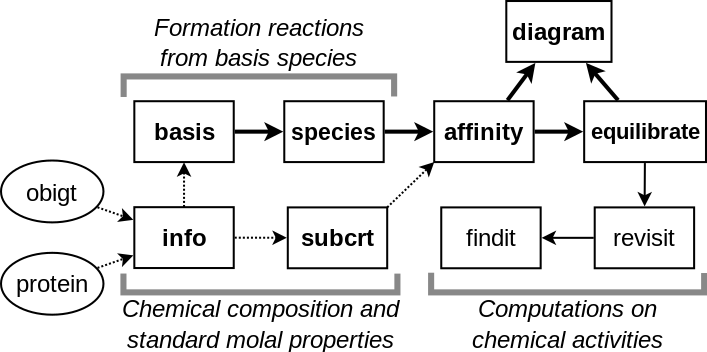
\includegraphics[width=0.75000\textwidth]{CHNOSZ.png}
\caption{Structure of CHNOSZ.}
\end{figure}

Many functions in CHNOSZ have no side effects. That is, the function
only returns a result; to use the result elsewhere, it can be assigned
to a variable with \texttt{\textless{}-}. In this document, the names of
these functions are set in {green text} (not applicable to the code
chunks).

\begin{marginfigure}
When they are mentioned, names of functions in the base and recommended
packages of R are said to belong to R. Example: Use R's \texttt{plot()}
to plot the data.
\end{marginfigure}

Major functions without side effects in CHNOSZ are:

\begin{itemize}
\tightlist
\item
  {\texttt{info()}}: search for species in the thermodynamic database;
\item
  {\texttt{subcrt()}}: calculate the thermodynamic properties of species
  and reactions;
\item
  {\texttt{affinity()}}: calculate the affinities of formation reactions
  using given chemical activities;
\item
  {\texttt{equilibrate()}}: calculate the equilibrium chemical
  activities of the species of interest;
\item
  {\texttt{diagram()}}: plot the results.
\end{itemize}

Some functions in CHNOSZ do have side effects: they modify the
\texttt{thermo} data object in the current R session. In this document,
the names of these functions are set in {red text} (but not in the code
chunks). Major functions with side effects are:

\begin{itemize}
\tightlist
\item
  {\texttt{basis()}}: set the basis species and their chemical
  activities;
\item
  {\texttt{species()}}: set the species of interest and their
  (non-equilibrium) chemical activities;
\item
  {\texttt{data(thermo)}}: reset the database, restoring all settings to
  their default values.
\end{itemize}

The following pseudocode shows a common sequence of commands. In actual
usage, the \texttt{...} are replaced by arguments that define the
chemical species and variables:

\begin{Shaded}
\begin{Highlighting}[]
\KeywordTok{data}\NormalTok{(thermo)         ## initialize system settings}
\KeywordTok{basis}\NormalTok{(...)}
\KeywordTok{species}\NormalTok{(...)}
\NormalTok{a <-}\StringTok{ }\KeywordTok{affinity}\NormalTok{(...)}
\NormalTok{e <-}\StringTok{ }\KeywordTok{equilibrate}\NormalTok{(a)  ## optional}
\KeywordTok{diagram}\NormalTok{(e)           ## or diagram(a)}
\KeywordTok{data}\NormalTok{(thermo)         ## clear settings for next calculation}
\end{Highlighting}
\end{Shaded}

\section{The basics}\label{the-basics}

\begin{itemize}
\tightlist
\item
  Use {\texttt{info()}} to search the thermodynamic database.
\end{itemize}

\begin{Shaded}
\begin{Highlighting}[]
\KeywordTok{info}\NormalTok{(}\StringTok{"aden "}\NormalTok{)}
\end{Highlighting}
\end{Shaded}

\begin{verbatim}
## [1] NA
\end{verbatim}

\begin{Shaded}
\begin{Highlighting}[]
\KeywordTok{info}\NormalTok{(}\StringTok{"adenine"}\NormalTok{)}
\end{Highlighting}
\end{Shaded}

\begin{verbatim}
## [1] 1675
\end{verbatim}

\begin{Shaded}
\begin{Highlighting}[]
\NormalTok{iadenine <-}\StringTok{ }\KeywordTok{info}\NormalTok{(}\StringTok{"adenine"}\NormalTok{)}
\end{Highlighting}
\end{Shaded}

\begin{Shaded}
\begin{Highlighting}[]
\KeywordTok{info}\NormalTok{(iadenine)}
\end{Highlighting}
\end{Shaded}

\begin{verbatim}
##         name abbrv formula state        ref1  ref2      date     G     H     S
## 1675 adenine  <NA>  C5H5N5    aq LH06a [S07] LCT17 26.Jul.17 74770 31235 53.41
##         Cp    V    a1 a2     a3 a4    c1     c2   omega Z
## 1675 51.63 90.6 2.353  0 -17.75  0 48.54 -33180 -109300 0
\end{verbatim}

\begin{itemize}
\tightlist
\item
  Use {\texttt{thermo.refs()}} to look up references.
\end{itemize}

\begin{Shaded}
\begin{Highlighting}[]
\KeywordTok{thermo.refs}\NormalTok{(iadenine)}
\end{Highlighting}
\end{Shaded}

\begin{verbatim}
##       key                                   author year
## 99  LH06a          D. E. LaRowe and H. C. Helgeson 2006
## 152 LCT17 A. R. Lowe, J. S. Cox and P. R. Tremaine 2017
##                                   citation
## 99  Geochim. Cosmochim. Acta 70, 4680-4724
## 152   J. Chem. Thermodynamics 112, 129-145
##                                                 note
## 99  nucleic-acid bases, nucleosides, and nucleotides
## 152                           adenine HKF parameters
##                                           URL
## 99  https://doi.org/10.1016/j.gca.2006.04.010
## 152 https://doi.org/10.1016/j.jct.2017.04.005
\end{verbatim}

\begin{itemize}
\tightlist
\item
  Use {\texttt{subcrt()}} to calculate standard molal thermodynamic
  properties.
\end{itemize}

\begin{marginfigure}
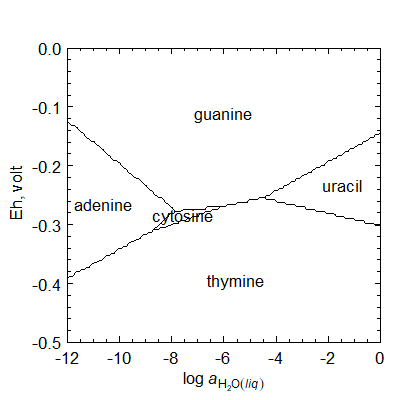
\includegraphics[width=1\linewidth]{anintro_chnosz_files/figure-latex/bsad_adenine-1} \caption[Nucleobase equal-activity diagram]{Nucleobase equal-activity diagram.}\label{fig:bsad_adenine}
\end{marginfigure}

\begin{Shaded}
\begin{Highlighting}[]
\KeywordTok{subcrt}\NormalTok{(}\StringTok{"adenine"}\NormalTok{, }\DataTypeTok{T =} \DecValTok{100}\NormalTok{)}
\end{Highlighting}
\end{Shaded}

\begin{verbatim}
## $species
##         name formula state ispecies
## 1675 adenine  C5H5N5    aq     1675
## 
## $out
## $out$adenine
##     T       P      rho     logK     G       H       S       V      Cp
## 1 100 1.01322 0.958393 -41.1609 70279 35542.8 66.2548 98.5326 62.4799
\end{verbatim}

\begin{marginfigure}
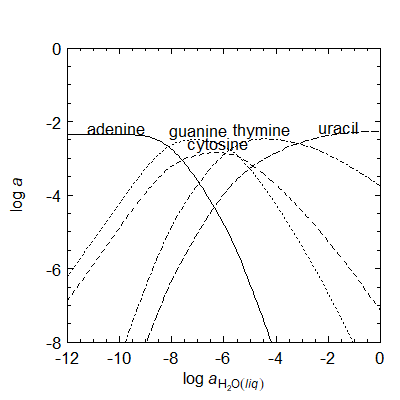
\includegraphics[width=1\linewidth]{anintro_chnosz_files/figure-latex/equil_adenine-1} \caption[Activities of nucleobases in metastable equilibrium]{Activities of nucleobases in metastable equilibrium.}\label{fig:equil_adenine}
\end{marginfigure}

\begin{itemize}
\tightlist
\item
  Use {\texttt{basis()}} -- {\texttt{species()}} --
  {\texttt{affinity()}} -- {\texttt{diagram()}} (BSAD) to construct
  equal-activity (equipotential) diagrams.
\end{itemize}

\begin{Shaded}
\begin{Highlighting}[]
\KeywordTok{basis}\NormalTok{(}\StringTok{"CHNOSe"}\NormalTok{)}
\KeywordTok{species}\NormalTok{(}\KeywordTok{c}\NormalTok{(}\StringTok{"adenine"}\NormalTok{, }\StringTok{"cytosine"}\NormalTok{, }\StringTok{"guanine"}\NormalTok{, }\StringTok{"thymine"}\NormalTok{, }\StringTok{"uracil"}\NormalTok{))}
\NormalTok{a <-}\StringTok{ }\KeywordTok{affinity}\NormalTok{(}\DataTypeTok{H2O =} \KeywordTok{c}\NormalTok{(}\OperatorTok{-}\DecValTok{12}\NormalTok{, }\OperatorTok{-}\DecValTok{0}\NormalTok{), }\DataTypeTok{Eh =} \KeywordTok{c}\NormalTok{(}\OperatorTok{-}\FloatTok{0.5}\NormalTok{, }\DecValTok{0}\NormalTok{), }\DataTypeTok{T =} \DecValTok{100}\NormalTok{)}
\KeywordTok{diagram}\NormalTok{(a)}
\end{Highlighting}
\end{Shaded}

\begin{itemize}
\tightlist
\item
  Use {\texttt{equilibrate()}} to calculate equilibrium activities.
\end{itemize}

\begin{Shaded}
\begin{Highlighting}[]
\KeywordTok{basis}\NormalTok{(}\StringTok{"e-"}\NormalTok{, }\FloatTok{3.6}\NormalTok{)}
\NormalTok{a <-}\StringTok{ }\KeywordTok{affinity}\NormalTok{(}\DataTypeTok{H2O =} \KeywordTok{c}\NormalTok{(}\OperatorTok{-}\DecValTok{12}\NormalTok{, }\DecValTok{0}\NormalTok{), }\DataTypeTok{T =} \DecValTok{100}\NormalTok{)}
\NormalTok{e <-}\StringTok{ }\KeywordTok{equilibrate}\NormalTok{(a)}
\KeywordTok{diagram}\NormalTok{(e, }\DataTypeTok{ylim =} \KeywordTok{c}\NormalTok{(}\OperatorTok{-}\DecValTok{8}\NormalTok{, }\DecValTok{0}\NormalTok{))}
\end{Highlighting}
\end{Shaded}

\section{Thermodynamic database}\label{thermodynamic-database}

An attempt has been made to provide a primary database (OBIGT) that has
no major inconsistencies. As the database includes datasets from many
sources, it can not be guaranteed to be fully internally consistent. For
crucial problems, check not only the accuracy of entries in the
database, but also the \emph{suitability of the data} for your problem.
If there are any doubts, consult the primary sources. Use
{\texttt{thermo.refs()}} to show a list of references for the data; see
also the vignette, \href{obigt.html}{{\emph{Thermodynamic data in
CHNOSZ}}}, for more information.

\subsection{\texorpdfstring{The {\texttt{info()}}
function}{The info() function}}\label{the-info-function}

{\texttt{info()}} provides an interface to the thermodynamic database
packaged with CHNOSZ. Suppose you are interested in the thermodynamic
properties of aqueous methane. You can search for the species by name:

\begin{Shaded}
\begin{Highlighting}[]
\KeywordTok{info}\NormalTok{(}\StringTok{"methane"}\NormalTok{)}
\end{Highlighting}
\end{Shaded}

\begin{verbatim}
## [1] 859
\end{verbatim}

Multiple entries exist for methane; the index of the \texttt{aq}
(aqueous) species is returned by default. A second argument can be used
to specify a different physical state:

\begin{Shaded}
\begin{Highlighting}[]
\KeywordTok{info}\NormalTok{(}\StringTok{"methane"}\NormalTok{, }\StringTok{"gas"}\NormalTok{)}
\end{Highlighting}
\end{Shaded}

\begin{verbatim}
## [1] 3307
\end{verbatim}

Knowing that aqueous methane is species number 859 in the database, you
can again use {\texttt{info()}} to retrieve the set of standard molal
thermodynamic properties and equations of state parameters:

\begin{Shaded}
\begin{Highlighting}[]
\KeywordTok{info}\NormalTok{(}\DecValTok{859}\NormalTok{)}
\end{Highlighting}
\end{Shaded}

\begin{verbatim}
##        name abbrv formula state       ref1 ref2      date     G      H  S    Cp
## 859 methane  <NA>     CH4    aq PS01 [S07] <NA> 04.Oct.00 -8140 -20930 21 60.23
##      V    a1    a2     a3     a4    c1    c2  omega Z
## 859 36 1.769 -1530 -67.88 114700 40.87 64500 -40000 0
\end{verbatim}

This number can be used as an argument (\texttt{ispecies}) for other
functions in CHNOSZ to uniquely identify any species; some commonly used
functions also accept the species names. Liquid water is species number
1; it has NA entries in the database because specialized functions are
used to compute its properties:

\begin{Shaded}
\begin{Highlighting}[]
\KeywordTok{info}\NormalTok{(}\KeywordTok{info}\NormalTok{(}\StringTok{"water"}\NormalTok{))}
\end{Highlighting}
\end{Shaded}

\begin{verbatim}
##    name abbrv formula state ref1 ref2      date  G  H  S Cp  V  a  b  c  d  e
## 1 water  <NA>     H2O   liq <NA> <NA> 25.Oct.06 NA NA NA NA NA NA NA NA NA NA
##    f lambda  T
## 1 NA     NA NA
\end{verbatim}

\subsection{Fuzzy searches}\label{fuzzy-searches}

Calling {\texttt{info()}} with a string that does not exactly match the
name of any species invokes a fuzzy search of the database:

\begin{Shaded}
\begin{Highlighting}[]
\KeywordTok{info}\NormalTok{(}\StringTok{"acid"}\NormalTok{)}
\end{Highlighting}
\end{Shaded}

\begin{verbatim}
## [1] NA
\end{verbatim}

The message includes e.g. ``uracil'' and ``metacinnabar'' because their
names have some similarity to the search term.

As ``ribose'' is the name of a species in the database, to find species
with similar names, add an extra character to the search:

\begin{Shaded}
\begin{Highlighting}[]
\KeywordTok{info}\NormalTok{(}\StringTok{" ribose"}\NormalTok{)}
\end{Highlighting}
\end{Shaded}

\begin{verbatim}
## [1] NA
\end{verbatim}

The messages may be useful for browsing the database, but owing to their
ambiguous results, these fuzzy searches return an \texttt{NA} value for
the species index.

\subsection{\texorpdfstring{Counting elements, chemical formulas,
{\texttt{ZC()}}}{Counting elements, chemical formulas, ZC()}}\label{counting-elements-chemical-formulas-zc}

Continuing with the example of methane, let's look at its chemical
formula:

\begin{Shaded}
\begin{Highlighting}[]
\KeywordTok{info}\NormalTok{(}\DecValTok{859}\NormalTok{)}\OperatorTok{$}\NormalTok{formula}
\end{Highlighting}
\end{Shaded}

\begin{verbatim}
## [1] "CH4"
\end{verbatim}

We can use {\texttt{makeup()}} to count the elements in the formula,
followed by {\texttt{as.chemical.formula()}} to rewrite the formula on
one line:

\begin{Shaded}
\begin{Highlighting}[]
\KeywordTok{makeup}\NormalTok{(}\DecValTok{859}\NormalTok{)}
\end{Highlighting}
\end{Shaded}

\begin{verbatim}
## C H 
## 1 4
\end{verbatim}

\begin{Shaded}
\begin{Highlighting}[]
\KeywordTok{as.chemical.formula}\NormalTok{(}\KeywordTok{makeup}\NormalTok{(}\DecValTok{859}\NormalTok{))}
\end{Highlighting}
\end{Shaded}

\begin{verbatim}
## [1] "CH4"
\end{verbatim}

For organic species, a calculation of the average oxidation state of
carbon (ZC) is possible given the species index, chemical formula, or
elemental count:

\begin{Shaded}
\begin{Highlighting}[]
\KeywordTok{ZC}\NormalTok{(}\DecValTok{859}\NormalTok{)}
\end{Highlighting}
\end{Shaded}

\begin{verbatim}
## [1] -4
\end{verbatim}

\begin{Shaded}
\begin{Highlighting}[]
\KeywordTok{ZC}\NormalTok{(}\KeywordTok{info}\NormalTok{(}\DecValTok{859}\NormalTok{)}\OperatorTok{$}\NormalTok{formula)}
\end{Highlighting}
\end{Shaded}

\begin{verbatim}
## [1] -4
\end{verbatim}

\begin{Shaded}
\begin{Highlighting}[]
\KeywordTok{ZC}\NormalTok{(}\KeywordTok{makeup}\NormalTok{(}\DecValTok{859}\NormalTok{))}
\end{Highlighting}
\end{Shaded}

\begin{verbatim}
## [1] -4
\end{verbatim}

\section{Calculating thermodynamic
properties}\label{calculating-thermodynamic-properties}

To calculate the standard molal properties of species and reactions, use
{\texttt{subcrt()}}.

\begin{marginfigure}
The inspiration for the name {\texttt{subcrt()}}, and the source of the
Fortran subroutine used to calculate the thermodynamic properties of
H2O, is SUPCRT (Johnson et al., 1992).
\end{marginfigure}

\citeyearpar{JOH92} If no reaction coefficients are given,
{\texttt{subcrt()}} calculates the standard molal properties of
individual species:

\begin{Shaded}
\begin{Highlighting}[]
\KeywordTok{subcrt}\NormalTok{(}\StringTok{"water"}\NormalTok{)}
\end{Highlighting}
\end{Shaded}

\begin{verbatim}
## $species
##    name formula state ispecies
## 1 water     H2O   liq        1
## 
## $out
## $out$water
##         T         P      rho    logK        G        H       S       V      Cp
## 1    0.01   1.00000 0.999829 45.0353 -56289.5 -68767.7 15.1324 18.0183 18.2056
## 2   25.00   1.00000 0.997061 41.5525 -56687.7 -68316.8 16.7123 18.0683 18.0116
## 3   50.00   1.00000 0.988030 38.6328 -57123.9 -67866.5 18.1623 18.2335 18.0046
## 4   75.00   1.00000 0.974864 36.1544 -57594.9 -67416.1 19.5048 18.4797 18.0416
## 5  100.00   1.01322 0.958393 34.0270 -58098.4 -66963.8 20.7596 18.7973 18.1579
## 6  125.00   2.32014 0.939073 32.1832 -58631.7 -66507.3 21.9419 19.1840 18.3333
## 7  150.00   4.75717 0.917058 30.5718 -59193.3 -66045.6 23.0640 19.6446 18.5664
## 8  175.00   8.91805 0.892343 29.1531 -59781.4 -65576.6 24.1360 20.1887 18.8830
## 9  200.00  15.53650 0.864743 27.8960 -60394.5 -65098.0 25.1682 20.8330 19.3288
## 10 225.00  25.47860 0.833873 26.7753 -61031.2 -64605.9 26.1712 21.6042 19.9704
## 11 250.00  39.73649 0.799072 25.7711 -61690.3 -64095.0 27.1569 22.5452 20.9123
## 12 275.00  59.43125 0.759236 24.8670 -62370.7 -63557.5 28.1400 23.7281 22.3513
## 13 300.00  85.83784 0.712408 24.0494 -63071.1 -62980.9 29.1407 25.2878 24.7394
## 14 325.00 120.45757 0.654577 23.3072 -63790.8 -62341.4 30.1952 27.5219 29.4475
## 15 350.00 165.21129 0.574688 22.6310 -64528.9 -61575.6 31.3971 31.3478 43.5985
\end{verbatim}

That uses the default temperature and pressure settings, i.e.~equally
spaced temperature intervals from 0 to 350 °C at \emph{P}sat.

\begin{marginfigure}
\emph{P}sat is 1 bar below 100 °C, or the pressure of liquid-vapor
saturation (i.e.~boiling) at higher temperatures.
\end{marginfigure}

The columns in the output are temperature, pressure, density of water,
logarithm of the equilibrium constant (only meaningful for reactions;
\protect\hyperlink{properties-of-reactions}{see below}), standard molal
Gibbs energy and enthalpy of formation from the elements, standard molal
entropy, volume, and heat capacity.

\begin{marginfigure}
The corresponding units are °C (\texttt{T}), bar (\texttt{P}), g cm-3
(\texttt{rho}), cal mol-1 (\texttt{G} and \texttt{H}), cal K-1 mol-1
(\texttt{S} and \texttt{Cp}), and cm3 mol-1 (\texttt{V}).
\end{marginfigure}

A custom temperature-pressure grid can be specified. Here, we calculate
the properties of H2O on a \emph{T}, \emph{P} grid in the supercritical
region, with conditions grouped by pressure:

\begin{marginfigure}
See also \href{../demo}{{\texttt{demo(density)}}}.
\end{marginfigure}

\begin{Shaded}
\begin{Highlighting}[]
\KeywordTok{subcrt}\NormalTok{(}\StringTok{"water"}\NormalTok{, }\DataTypeTok{T =} \KeywordTok{c}\NormalTok{(}\DecValTok{400}\NormalTok{, }\DecValTok{500}\NormalTok{, }\DecValTok{600}\NormalTok{), }\DataTypeTok{P =} \KeywordTok{c}\NormalTok{(}\DecValTok{200}\NormalTok{, }\DecValTok{400}\NormalTok{, }\DecValTok{600}\NormalTok{), }\DataTypeTok{grid =} \StringTok{"P"}\NormalTok{)}\OperatorTok{$}\NormalTok{out}\OperatorTok{$}\NormalTok{water}
\end{Highlighting}
\end{Shaded}

\begin{verbatim}
##     T   P       rho    logK        G        H       S        V      Cp
## 1 400 200 0.1005447 21.5271 -66306.4 -56639.3 39.0387 179.1760 27.4305
## 2 500 200 0.0677109 19.8868 -70353.7 -54819.8 41.5776 266.0607 14.0774
## 3 600 200 0.0550386 18.6704 -74593.1 -53540.0 43.1368 327.3197 11.9607
## 4 400 400 0.5236661 21.4119 -65951.4 -60454.4 32.8438  34.4021 37.5317
## 5 500 400 0.1779739 19.6639 -69565.0 -56252.5 38.7044 101.2238 24.9675
## 6 600 400 0.1238075 18.4124 -73562.4 -54361.7 41.0152 145.5098 15.4901
## 7 400 600 0.6124511 21.3631 -65801.3 -60832.4 32.0592  29.4149 25.8810
## 8 500 600 0.3384430 19.5660 -69218.6 -57694.2 36.3916  53.2296 32.4385
## 9 600 600 0.2071976 18.2784 -73027.2 -55195.1 39.4479  86.9469 19.3763
\end{verbatim}

\begin{marginfigure}
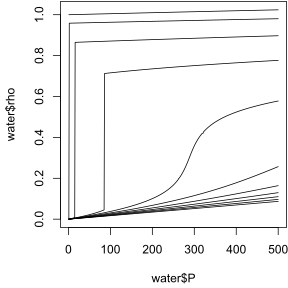
\includegraphics[width=1\linewidth]{anintro_chnosz_files/figure-latex/subcrt_water_plot-1} \caption[Isothermal contours of density (g cm<sup>-3</sup>) and pressure (bar) of water]{Isothermal contours of density (g cm<sup>-3</sup>) and pressure (bar) of water.}\label{fig:subcrt_water_plot}
\end{marginfigure}

The additional operations (\texttt{\$out\$water}) are used to extract a
specific part of the results; this can be used with e.g.~R's
\texttt{write.table()} or \texttt{plot()} for further processing:

\begin{Shaded}
\begin{Highlighting}[]
\NormalTok{substuff <-}\StringTok{ }\KeywordTok{subcrt}\NormalTok{(}\StringTok{"water"}\NormalTok{, }\DataTypeTok{T=}\KeywordTok{seq}\NormalTok{(}\DecValTok{0}\NormalTok{,}\DecValTok{1000}\NormalTok{,}\DecValTok{100}\NormalTok{), }\DataTypeTok{P=}\KeywordTok{c}\NormalTok{(}\OtherTok{NA}\NormalTok{, }\KeywordTok{seq}\NormalTok{(}\DecValTok{1}\NormalTok{,}\DecValTok{500}\NormalTok{,}\DecValTok{1}\NormalTok{)), }\DataTypeTok{grid=}\StringTok{"T"}\NormalTok{)}
\NormalTok{water <-}\StringTok{ }\NormalTok{substuff}\OperatorTok{$}\NormalTok{out}\OperatorTok{$}\NormalTok{water}
\KeywordTok{plot}\NormalTok{(water}\OperatorTok{$}\NormalTok{P, water}\OperatorTok{$}\NormalTok{rho, }\DataTypeTok{type =} \StringTok{"l"}\NormalTok{)}
\end{Highlighting}
\end{Shaded}

\subsection{Changing units}\label{changing-units}

The default units of temperature, pressure, and energy are °C, bar, and
calories. The functions {\texttt{T.units()}}, {\texttt{P.units()}}, and
{\texttt{E.units()}} can be used to change the units used by various
functions in CHNOSZ. What is the Gibbs energy in J/mol of aqueous
methane at 298.15 K and 0.1 MPa?

\begin{Shaded}
\begin{Highlighting}[]
\KeywordTok{T.units}\NormalTok{(}\StringTok{"K"}\NormalTok{)}
\KeywordTok{P.units}\NormalTok{(}\StringTok{"MPa"}\NormalTok{)}
\KeywordTok{E.units}\NormalTok{(}\StringTok{"J"}\NormalTok{)}
\KeywordTok{subcrt}\NormalTok{(}\StringTok{"methane"}\NormalTok{, }\DataTypeTok{T =} \FloatTok{298.15}\NormalTok{, }\DataTypeTok{P =} \FloatTok{0.1}\NormalTok{)}\OperatorTok{$}\NormalTok{out}\OperatorTok{$}\NormalTok{methane}\OperatorTok{$}\NormalTok{G}
\end{Highlighting}
\end{Shaded}

\begin{verbatim}
## [1] -34057.8
\end{verbatim}

A related function, {\texttt{convert()}}, can be used to convert given
values between units. Let's convert the standard Gibbs energy of aqueous
methane listed in the database from cal/mol to J/mol:

\begin{Shaded}
\begin{Highlighting}[]
\KeywordTok{convert}\NormalTok{(}\KeywordTok{info}\NormalTok{(}\KeywordTok{info}\NormalTok{(}\StringTok{"methane"}\NormalTok{))}\OperatorTok{$}\NormalTok{G, }\StringTok{"J"}\NormalTok{)}
\end{Highlighting}
\end{Shaded}

\begin{verbatim}
## [1] -34057.8
\end{verbatim}

As expected, we get the same result from both operations.

Use {\texttt{data(thermo)}} to restore the units and all other settings
for CHNOSZ to their defaults:

\begin{Shaded}
\begin{Highlighting}[]
\KeywordTok{data}\NormalTok{(thermo)}
\end{Highlighting}
\end{Shaded}

\hypertarget{properties-of-reactions}{\section{Properties of
reactions}\label{properties-of-reactions}}

\subsection{Reaction definitions}\label{reaction-definitions}

To calculate the thermodynamic properties of reactions, give the names
of species, the physical states (optional), and reaction coefficients as
the arguments to {\texttt{subcrt()}}. Here we calculate properties for
the dissolution of CO2:

\begin{marginfigure}
Because of aqueous speciation, this doesn't give the \emph{solubility}
of CO2. For an example of a solubility calculation, see
\href{../demo}{{\texttt{demo(solubility)}}}, which is based on a figure
in Manning et al. (2013).
\end{marginfigure}

\begin{Shaded}
\begin{Highlighting}[]
\KeywordTok{subcrt}\NormalTok{(}\KeywordTok{c}\NormalTok{(}\StringTok{"CO2"}\NormalTok{, }\StringTok{"CO2"}\NormalTok{), }\KeywordTok{c}\NormalTok{(}\StringTok{"gas"}\NormalTok{, }\StringTok{"aq"}\NormalTok{), }\KeywordTok{c}\NormalTok{(}\OperatorTok{-}\DecValTok{1}\NormalTok{, }\DecValTok{1}\NormalTok{), }\DataTypeTok{T =} \KeywordTok{seq}\NormalTok{(}\DecValTok{0}\NormalTok{, }\DecValTok{250}\NormalTok{, }\DecValTok{50}\NormalTok{))}
\end{Highlighting}
\end{Shaded}

\begin{verbatim}
## $reaction
##      coeff           name formula state ispecies
## 3308    -1 carbon dioxide     CO2   gas     3308
## 1576     1            CO2     CO2    aq     1576
## 
## $out
##        T        P      rho     logK       G         H         S       V      Cp
## 1   0.01  1.00000 0.999829 -1.10873 1385.80 -5907.949 -26.70130 23.6978 49.1458
## 2  50.00  1.00000 0.988030 -1.71865 2541.27 -3947.724 -20.08036 36.9843 34.6260
## 3 100.00  1.01322 0.958393 -2.00354 3420.89 -2271.995 -15.25623 41.5584 33.0446
## 4 150.00  4.75717 0.917058 -2.10770 4080.94  -596.111 -11.05290 44.5642 34.3421
## 5 200.00 15.53650 0.864743 -2.09920 4544.74  1228.815  -7.00814 47.9553 39.3857
## 6 250.00 39.73649 0.799072 -2.01184 4815.90  3513.101  -2.49026 54.3882 55.7180
\end{verbatim}

In order to make a plot like Figure 18 of \citet{MSS13}, let's run more
calculations and store the results. In addition to the reaction
definition, we specify a greater number of temperature points than the
default:

\begin{marginfigure}
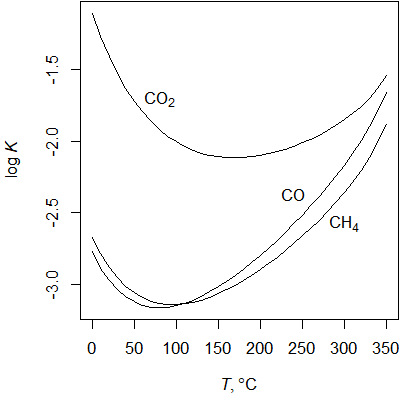
\includegraphics[width=1\linewidth]{anintro_chnosz_files/figure-latex/CO2_plot-1} \caption[Calculated equilibrium constants for dissolution of CO<sub>2</sub>, CO, and CH<sub>4</sub>]{Calculated equilibrium constants for dissolution of CO<sub>2</sub>, CO, and CH<sub>4</sub>.}\label{fig:CO2_plot}
\end{marginfigure}

\begin{Shaded}
\begin{Highlighting}[]
\NormalTok{T <-}\StringTok{ }\KeywordTok{seq}\NormalTok{(}\DecValTok{0}\NormalTok{, }\DecValTok{350}\NormalTok{, }\DecValTok{10}\NormalTok{)}
\NormalTok{CO2 <-}\StringTok{ }\KeywordTok{subcrt}\NormalTok{(}\KeywordTok{c}\NormalTok{(}\StringTok{"CO2"}\NormalTok{, }\StringTok{"CO2"}\NormalTok{), }\KeywordTok{c}\NormalTok{(}\StringTok{"gas"}\NormalTok{, }\StringTok{"aq"}\NormalTok{), }\KeywordTok{c}\NormalTok{(}\OperatorTok{-}\DecValTok{1}\NormalTok{, }\DecValTok{1}\NormalTok{), }\DataTypeTok{T =}\NormalTok{ T)}\OperatorTok{$}\NormalTok{out}\OperatorTok{$}\NormalTok{logK}
\NormalTok{CO <-}\StringTok{ }\KeywordTok{subcrt}\NormalTok{(}\KeywordTok{c}\NormalTok{(}\StringTok{"CO"}\NormalTok{, }\StringTok{"CO"}\NormalTok{), }\KeywordTok{c}\NormalTok{(}\StringTok{"gas"}\NormalTok{, }\StringTok{"aq"}\NormalTok{), }\KeywordTok{c}\NormalTok{(}\OperatorTok{-}\DecValTok{1}\NormalTok{, }\DecValTok{1}\NormalTok{), }\DataTypeTok{T =}\NormalTok{ T)}\OperatorTok{$}\NormalTok{out}\OperatorTok{$}\NormalTok{logK}
\NormalTok{CH4 <-}\StringTok{ }\KeywordTok{subcrt}\NormalTok{(}\KeywordTok{c}\NormalTok{(}\StringTok{"CH4"}\NormalTok{, }\StringTok{"CH4"}\NormalTok{), }\KeywordTok{c}\NormalTok{(}\StringTok{"gas"}\NormalTok{, }\StringTok{"aq"}\NormalTok{), }\KeywordTok{c}\NormalTok{(}\OperatorTok{-}\DecValTok{1}\NormalTok{, }\DecValTok{1}\NormalTok{), }\DataTypeTok{T =}\NormalTok{ T)}\OperatorTok{$}\NormalTok{out}\OperatorTok{$}\NormalTok{logK}
\NormalTok{logK <-}\StringTok{ }\KeywordTok{data.frame}\NormalTok{(T, CO2, CO, CH4)}
\end{Highlighting}
\end{Shaded}

Now we can make the plot, using R's \texttt{matplot()}. Here,
{\texttt{axis.label()}} and {\texttt{expr.species()}} are used to create
formatted axis labels and chemical formulas:

\begin{Shaded}
\begin{Highlighting}[]
\KeywordTok{matplot}\NormalTok{(logK[, }\DecValTok{1}\NormalTok{], logK[, }\OperatorTok{-}\DecValTok{1}\NormalTok{], }\DataTypeTok{type =} \StringTok{"l"}\NormalTok{, }\DataTypeTok{col =} \DecValTok{1}\NormalTok{, }\DataTypeTok{lty =} \DecValTok{1}\NormalTok{,}
        \DataTypeTok{xlab =} \KeywordTok{axis.label}\NormalTok{(}\StringTok{"T"}\NormalTok{), }\DataTypeTok{ylab =} \KeywordTok{axis.label}\NormalTok{(}\StringTok{"logK"}\NormalTok{))}
\KeywordTok{text}\NormalTok{(}\DecValTok{80}\NormalTok{, }\OperatorTok{-}\FloatTok{1.7}\NormalTok{, }\KeywordTok{expr.species}\NormalTok{(}\StringTok{"CO2"}\NormalTok{))}
\KeywordTok{text}\NormalTok{(}\DecValTok{240}\NormalTok{, }\OperatorTok{-}\FloatTok{2.37}\NormalTok{, }\KeywordTok{expr.species}\NormalTok{(}\StringTok{"CO"}\NormalTok{))}
\KeywordTok{text}\NormalTok{(}\DecValTok{300}\NormalTok{, }\OperatorTok{-}\FloatTok{2.57}\NormalTok{, }\KeywordTok{expr.species}\NormalTok{(}\StringTok{"CH4"}\NormalTok{))}
\end{Highlighting}
\end{Shaded}

\subsection{Unbalanced reactions}\label{unbalanced-reactions}

A balanced chemical reaction conserves mass. {\texttt{subcrt()}} won't
stop you from running an unbalanced reaction, but it will give you a
warning:

\begin{Shaded}
\begin{Highlighting}[]
\KeywordTok{subcrt}\NormalTok{(}\KeywordTok{c}\NormalTok{(}\StringTok{"CO2"}\NormalTok{, }\StringTok{"CH4"}\NormalTok{), }\KeywordTok{c}\NormalTok{(}\OperatorTok{-}\DecValTok{1}\NormalTok{, }\DecValTok{1}\NormalTok{))}
\end{Highlighting}
\end{Shaded}

In other words, to balance the reaction, we should add 4 H to the left
and 2 O to the right. That could be done manually be redefining the
reaction with the appropriate species. There is another option:
balancing the reaction automatically using basis species.

\subsection{Setting the basis species}\label{setting-the-basis-species}

\emph{Basis species} are a minimal number of chemical species that
linearly combine to give the composition of any species in the system.
The basis species are similar to thermodynamic components, but can
include charged species. Basis species are used in CHNOSZ to
automatically balance reactions; they are also required for making
chemical activity diagrams.

Let's start with an example that doesn't work:

\begin{Shaded}
\begin{Highlighting}[]
\KeywordTok{basis}\NormalTok{(}\KeywordTok{c}\NormalTok{(}\StringTok{"CO2"}\NormalTok{, }\StringTok{"H2"}\NormalTok{, }\StringTok{"H2CO2"}\NormalTok{))}
\end{Highlighting}
\end{Shaded}

That set of species has a singular (non-invertible) stoichiometric
matrix. An error would also result from either an underdetermined or
overdetermined system. A valid set of basis species has an invertible
stoichiometric matrix and the same number of species as elements:

\begin{Shaded}
\begin{Highlighting}[]
\KeywordTok{basis}\NormalTok{(}\KeywordTok{c}\NormalTok{(}\StringTok{"CO2"}\NormalTok{, }\StringTok{"H2"}\NormalTok{, }\StringTok{"H2O"}\NormalTok{))}
\end{Highlighting}
\end{Shaded}

\begin{verbatim}
##     C H O ispecies logact state
## CO2 1 0 2     1576      0    aq
## H2  0 2 0       64      0    aq
## H2O 0 2 1        1      0   liq
\end{verbatim}

The composition of any species made up of C, H, and O can be represented
by a single linear combination of these basis species.

\subsection{Automatically balancing
reactions}\label{automatically-balancing-reactions}

Methanogenic metabolism in reducing environments may proceed by
acetoclastic or hydrogenotrophic processes. To consider reactions
involving a charged species (acetate), let's define a basis with H+:

\begin{Shaded}
\begin{Highlighting}[]
\KeywordTok{basis}\NormalTok{(}\KeywordTok{c}\NormalTok{(}\StringTok{"CO2"}\NormalTok{, }\StringTok{"H2"}\NormalTok{, }\StringTok{"H2O"}\NormalTok{, }\StringTok{"H+"}\NormalTok{))}
\end{Highlighting}
\end{Shaded}

\begin{verbatim}
##     C H O Z ispecies logact state
## CO2 1 0 2 0     1576      0    aq
## H2  0 2 0 0       64      0    aq
## H2O 0 2 1 0        1      0   liq
## H+  0 1 0 1        3      0    aq
\end{verbatim}

By identifying species \emph{other than} the basis species, the
reactions will be automatically balanced. This produces the balanced
reaction for acetoclastic methanogenesis:

\begin{Shaded}
\begin{Highlighting}[]
\KeywordTok{subcrt}\NormalTok{(}\KeywordTok{c}\NormalTok{(}\StringTok{"acetate"}\NormalTok{, }\StringTok{"methane"}\NormalTok{), }\KeywordTok{c}\NormalTok{(}\OperatorTok{-}\DecValTok{1}\NormalTok{, }\DecValTok{1}\NormalTok{))}\OperatorTok{$}\NormalTok{reaction}
\end{Highlighting}
\end{Shaded}

\begin{verbatim}
##      coeff    name formula state ispecies
## 1070    -1 acetate C2H3O2-    aq     1070
## 859      1 methane     CH4    aq      859
## 1576     1     CO2     CO2    aq     1576
## 3       -1      H+      H+    aq        3
\end{verbatim}

We can similarly consider reactions for hydrogenotrophic methanogenesis
as well as acetate oxidation (without production of methane):

\begin{Shaded}
\begin{Highlighting}[]
\NormalTok{acetate_oxidation <-}\StringTok{ }\KeywordTok{subcrt}\NormalTok{(}\StringTok{"acetate"}\NormalTok{, }\OperatorTok{-}\DecValTok{1}\NormalTok{)}
\NormalTok{hydrogenotrophic <-}\StringTok{ }\KeywordTok{subcrt}\NormalTok{(}\StringTok{"methane"}\NormalTok{, }\DecValTok{1}\NormalTok{)}
\NormalTok{acetoclastic <-}\StringTok{ }\KeywordTok{subcrt}\NormalTok{(}\KeywordTok{c}\NormalTok{(}\StringTok{"acetate"}\NormalTok{, }\StringTok{"methane"}\NormalTok{), }\KeywordTok{c}\NormalTok{(}\OperatorTok{-}\DecValTok{1}\NormalTok{, }\DecValTok{1}\NormalTok{))}
\end{Highlighting}
\end{Shaded}

Use {\texttt{describe.reaction()}} to write the reactions on a plot:

\begin{marginfigure}
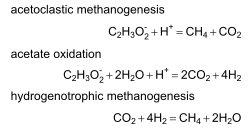
\includegraphics[width=1\linewidth]{anintro_chnosz_files/figure-latex/describe_reaction_plot-1} \end{marginfigure}

\begin{Shaded}
\begin{Highlighting}[]
\KeywordTok{plot}\NormalTok{(}\DecValTok{0}\NormalTok{, }\DecValTok{0}\NormalTok{, }\DataTypeTok{type =} \StringTok{"n"}\NormalTok{, }\DataTypeTok{axes =} \OtherTok{FALSE}\NormalTok{, }\DataTypeTok{ann=}\OtherTok{FALSE}\NormalTok{, }\DataTypeTok{xlim=}\KeywordTok{c}\NormalTok{(}\DecValTok{0}\NormalTok{, }\DecValTok{5}\NormalTok{), }\DataTypeTok{ylim=}\KeywordTok{c}\NormalTok{(}\FloatTok{5.2}\NormalTok{, }\OperatorTok{-}\FloatTok{0.2}\NormalTok{))}
\KeywordTok{text}\NormalTok{(}\DecValTok{0}\NormalTok{, }\DecValTok{0}\NormalTok{, }\StringTok{"acetoclastic methanogenesis"}\NormalTok{, }\DataTypeTok{adj =} \DecValTok{0}\NormalTok{)}
\KeywordTok{text}\NormalTok{(}\DecValTok{5}\NormalTok{, }\DecValTok{1}\NormalTok{, }\KeywordTok{describe.reaction}\NormalTok{(acetoclastic}\OperatorTok{$}\NormalTok{reaction), }\DataTypeTok{adj =} \DecValTok{1}\NormalTok{)}
\KeywordTok{text}\NormalTok{(}\DecValTok{0}\NormalTok{, }\DecValTok{2}\NormalTok{, }\StringTok{"acetate oxidation"}\NormalTok{, }\DataTypeTok{adj =} \DecValTok{0}\NormalTok{)}
\KeywordTok{text}\NormalTok{(}\DecValTok{5}\NormalTok{, }\DecValTok{3}\NormalTok{, }\KeywordTok{describe.reaction}\NormalTok{(acetate_oxidation}\OperatorTok{$}\NormalTok{reaction), }\DataTypeTok{adj =} \DecValTok{1}\NormalTok{)}
\KeywordTok{text}\NormalTok{(}\DecValTok{0}\NormalTok{, }\DecValTok{4}\NormalTok{, }\StringTok{"hydrogenotrophic methanogenesis"}\NormalTok{, }\DataTypeTok{adj =} \DecValTok{0}\NormalTok{)}
\KeywordTok{text}\NormalTok{(}\DecValTok{5}\NormalTok{, }\DecValTok{5}\NormalTok{, }\KeywordTok{describe.reaction}\NormalTok{(hydrogenotrophic}\OperatorTok{$}\NormalTok{reaction), }\DataTypeTok{adj =} \DecValTok{1}\NormalTok{)}
\end{Highlighting}
\end{Shaded}

\subsection{Chemical affinity}\label{chemical-affinity}

Usually, {\texttt{subcrt()}} returns only standard state thermodynamic
properties.

\begin{marginfigure}
The standard state adopted for H2O is unit activity of the pure
component at any \emph{T} and \emph{P}. The standard state for aqueous
species is unit activity of a hypothetical one molal solution referenced
to infinite dilution at any \emph{T} and \emph{P}.
\end{marginfigure}

Thermodynamic models often consider a non-standard state (i.e.~non-unit
activity). The activities of basis species can be modified with
{\texttt{basis()}}, and those of the other species using the
\texttt{logact} argument in {\texttt{subcrt()}}.

Let us calculate the chemical affinity of acetoclastic methanogenesis.

\begin{marginfigure}
The affinity is equal to the negative of the overall (non-standard)
Gibbs energy change of the reaction.
\end{marginfigure}

We begin by changing the energy units to Joules. Then, we change the
state of H2O and CO2 in the basis from \texttt{aq} (aqueous) to
\texttt{gas}, and set the logarithm of fugacity of gaseous H2 and the
pH, using values from \citet{MDS_13}. The activity of acetate and
fugacity of methane, as well as temperature and pressure, are set in the
call to {\texttt{subcrt()}}:

\begin{Shaded}
\begin{Highlighting}[]
\KeywordTok{E.units}\NormalTok{(}\StringTok{"J"}\NormalTok{)}
\KeywordTok{basis}\NormalTok{(}\KeywordTok{c}\NormalTok{(}\StringTok{"CO2"}\NormalTok{, }\StringTok{"H2"}\NormalTok{, }\StringTok{"H2O"}\NormalTok{, }\StringTok{"H+"}\NormalTok{))}
\KeywordTok{basis}\NormalTok{(}\KeywordTok{c}\NormalTok{(}\StringTok{"CO2"}\NormalTok{, }\StringTok{"H2"}\NormalTok{), }\StringTok{"gas"}\NormalTok{)}
\KeywordTok{basis}\NormalTok{(}\KeywordTok{c}\NormalTok{(}\StringTok{"H2"}\NormalTok{, }\StringTok{"pH"}\NormalTok{), }\KeywordTok{c}\NormalTok{(}\OperatorTok{-}\FloatTok{3.92}\NormalTok{, }\FloatTok{7.3}\NormalTok{))}
\end{Highlighting}
\end{Shaded}

\begin{Shaded}
\begin{Highlighting}[]
\KeywordTok{subcrt}\NormalTok{(}\KeywordTok{c}\NormalTok{(}\StringTok{"acetate"}\NormalTok{, }\StringTok{"methane"}\NormalTok{), }\KeywordTok{c}\NormalTok{(}\OperatorTok{-}\DecValTok{1}\NormalTok{, }\DecValTok{1}\NormalTok{),}
       \KeywordTok{c}\NormalTok{(}\StringTok{"aq"}\NormalTok{, }\StringTok{"gas"}\NormalTok{), }\DataTypeTok{logact =} \KeywordTok{c}\NormalTok{(}\OperatorTok{-}\FloatTok{3.4}\NormalTok{, }\OperatorTok{-}\FloatTok{0.18}\NormalTok{), }\DataTypeTok{T =} \DecValTok{55}\NormalTok{, }\DataTypeTok{P =} \DecValTok{50}\NormalTok{)}\OperatorTok{$}\NormalTok{out}
\end{Highlighting}
\end{Shaded}

\begin{verbatim}
##    T  P      rho    logK        G       H       S        V      Cp  logQ
## 1 55 50 0.987821 13.5984 -85429.6 18706.9 317.685 -40.1339 39.2144 10.52
##         A
## 1 19339.4
\end{verbatim}

The new \texttt{A} column shows the affinity; the other columns are
unaffected and still show the standard-state properties. Let's repeat
the calculation for hydrogenotrophic methanogenesis.

\begin{Shaded}
\begin{Highlighting}[]
\KeywordTok{subcrt}\NormalTok{(}\StringTok{"methane"}\NormalTok{, }\DecValTok{1}\NormalTok{, }\StringTok{"gas"}\NormalTok{, }\DataTypeTok{logact =} \OperatorTok{-}\FloatTok{0.18}\NormalTok{, }\DataTypeTok{T =} \DecValTok{55}\NormalTok{, }\DataTypeTok{P =} \DecValTok{50}\NormalTok{)}\OperatorTok{$}\NormalTok{out}
\end{Highlighting}
\end{Shaded}

\begin{verbatim}
##    T  P      rho   logK       G       H        S       V      Cp logQ       A
## 1 55 50 0.987821 18.828 -118284 -251807 -407.195 36.4746 33.4702 15.5 20907.8
\end{verbatim}

Under the specified conditions, the affinities of hydrogenotrophic and
acetoclastic methanogenesis are somewhat greater than and less than 20
kJ, respectively. This result matches Figure 4b in Mayumi et al. (2013)
at unit fugacity of CO2.

We can go even further and reproduce their plot.

\begin{marginfigure}
The reproduction is not identical, owing to differences of thermodynamic
data and of calculations of the effects of temperature and pressure.
\end{marginfigure}

To make the code neater, we write a function that can run any of the
reactions:

\begin{Shaded}
\begin{Highlighting}[]
\NormalTok{rxnfun <-}\StringTok{ }\ControlFlowTok{function}\NormalTok{(coeffs) \{}
  \KeywordTok{subcrt}\NormalTok{(}\KeywordTok{c}\NormalTok{(}\StringTok{"acetate"}\NormalTok{, }\StringTok{"methane"}\NormalTok{), coeffs,}
         \KeywordTok{c}\NormalTok{(}\StringTok{"aq"}\NormalTok{, }\StringTok{"gas"}\NormalTok{), }\DataTypeTok{logact =} \KeywordTok{c}\NormalTok{(}\OperatorTok{-}\FloatTok{3.4}\NormalTok{, }\OperatorTok{-}\FloatTok{0.18}\NormalTok{), }\DataTypeTok{T =} \DecValTok{55}\NormalTok{, }\DataTypeTok{P =} \DecValTok{50}\NormalTok{)}\OperatorTok{$}\NormalTok{out}
\NormalTok{\}}
\end{Highlighting}
\end{Shaded}

Now we're ready to calculate and plot the affinities. Here, we use R's
\texttt{lapply()} to list the results at two values of logarithm of
fugacity of CO2. We insert an empty reaction to get a line at zero
affinity. R's \texttt{do.call()} and \texttt{rbind()} are used to turn
the list into a data frame that can be plotted with R's
\texttt{matplot()}. There, we plot the negative affinities, equal to
Gibbs energy, as shown in the plot of Mayumi et al. (2013).

\begin{marginfigure}
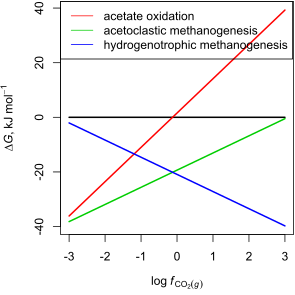
\includegraphics[width=1\linewidth]{anintro_chnosz_files/figure-latex/methanogenesis_plot-1} \caption[Gibbs energies of acetate oxidation and methanogenesis (after Mayumi et al., 2013)]{Gibbs energies of acetate oxidation and methanogenesis (after Mayumi et al., 2013).}\label{fig:methanogenesis_plot}
\end{marginfigure}

\begin{Shaded}
\begin{Highlighting}[]
\NormalTok{Adat <-}\StringTok{ }\KeywordTok{lapply}\NormalTok{(}\KeywordTok{c}\NormalTok{(}\OperatorTok{-}\DecValTok{3}\NormalTok{, }\DecValTok{3}\NormalTok{), }\ControlFlowTok{function}\NormalTok{(logfCO2) \{}
  \KeywordTok{basis}\NormalTok{(}\StringTok{"CO2"}\NormalTok{, logfCO2)}
  \KeywordTok{data.frame}\NormalTok{(logfCO2,}
    \KeywordTok{rxnfun}\NormalTok{(}\KeywordTok{c}\NormalTok{(}\DecValTok{0}\NormalTok{, }\DecValTok{0}\NormalTok{))}\OperatorTok{$}\NormalTok{A,}
    \KeywordTok{rxnfun}\NormalTok{(}\KeywordTok{c}\NormalTok{(}\OperatorTok{-}\DecValTok{1}\NormalTok{, }\DecValTok{0}\NormalTok{))}\OperatorTok{$}\NormalTok{A,}
    \KeywordTok{rxnfun}\NormalTok{(}\KeywordTok{c}\NormalTok{(}\OperatorTok{-}\DecValTok{1}\NormalTok{, }\DecValTok{1}\NormalTok{))}\OperatorTok{$}\NormalTok{A,}
    \KeywordTok{rxnfun}\NormalTok{(}\KeywordTok{c}\NormalTok{(}\DecValTok{0}\NormalTok{, }\DecValTok{1}\NormalTok{))}\OperatorTok{$}\NormalTok{A}
\NormalTok{  )}
\NormalTok{\})}
\NormalTok{Adat <-}\StringTok{ }\KeywordTok{do.call}\NormalTok{(rbind, Adat)}
\KeywordTok{matplot}\NormalTok{(Adat[, }\DecValTok{1}\NormalTok{], }\OperatorTok{-}\NormalTok{Adat[, }\OperatorTok{-}\DecValTok{1}\NormalTok{]}\OperatorTok{/}\DecValTok{1000}\NormalTok{, }\DataTypeTok{type =} \StringTok{"l"}\NormalTok{, }\DataTypeTok{lty =} \DecValTok{1}\NormalTok{, }\DataTypeTok{lwd =} \DecValTok{2}\NormalTok{,}
  \DataTypeTok{xlab =} \KeywordTok{axis.label}\NormalTok{(}\StringTok{"CO2"}\NormalTok{), }\DataTypeTok{ylab =} \KeywordTok{axis.label}\NormalTok{(}\StringTok{"DG"}\NormalTok{, }\DataTypeTok{prefix =} \StringTok{"k"}\NormalTok{))}
\KeywordTok{legend}\NormalTok{(}\StringTok{"topleft"}\NormalTok{, }\KeywordTok{c}\NormalTok{(}\StringTok{"acetate oxidation"}\NormalTok{, }\StringTok{"acetoclastic methanogenesis"}\NormalTok{,}
  \StringTok{"hydrogenotrophic methanogenesis"}\NormalTok{), }\DataTypeTok{lty =} \DecValTok{1}\NormalTok{, }\DataTypeTok{col =} \DecValTok{2}\OperatorTok{:}\DecValTok{4}\NormalTok{)}
\end{Highlighting}
\end{Shaded}

Let's not forget to clear the system settings, which were modified by
{\texttt{basis()}} and {\texttt{E.units()}}, before running other
calculations:

\begin{Shaded}
\begin{Highlighting}[]
\KeywordTok{data}\NormalTok{(thermo)}
\end{Highlighting}
\end{Shaded}

\section{\texorpdfstring{Using
{\texttt{affinity()}}}{Using affinity()}}\label{using-affinity}

{\texttt{affinity()}} offers calculations of chemical affinity of
formation reactions over a configurable range of \emph{T}, \emph{P}, and
activities of basis species.

\hypertarget{species-of-interest}{\subsection{Species of
interest}\label{species-of-interest}}

By \emph{formation reaction} is meant the stoichiometric requirements
for formation of one mole of any species from the basis species. The
{\texttt{species()}} function is used to set these \emph{species of
interest}. Let's consider the stoichiometry of some aqueous
sulfur-bearing species. Here we use {\texttt{basis()}} with a keyword to
load a preset basis definition.

\begin{marginfigure}
Some available keywords are \texttt{CHNOS} (including CO2, H2O, NH3,
H2S, and O2), \texttt{CHNOS+} (also including H+), and \texttt{CHNOSe}
(including H+, and \emph{e}- instead of O2). See {\texttt{?basis}} for
more options.
\end{marginfigure}\begin{marginfigure}
What is \texttt{SO42-}? Is it 1 S, 4 O, and 2 negative charges, or 1 S,
42 O, and 1 negative charge? The ambiguity of a digit that could belong
to the coefficient for the following charge or to that for the preceding
element is why formulas in CHNOSZ are written with the number of charges
after the + or - symbol. \texttt{SO4-2} is unambiguously parsed as 1 S,
4 O and 2 negative charges.
\end{marginfigure}

\begin{Shaded}
\begin{Highlighting}[]
\KeywordTok{basis}\NormalTok{(}\StringTok{"CHNOS+"}\NormalTok{)}
\end{Highlighting}
\end{Shaded}

\begin{Shaded}
\begin{Highlighting}[]
\KeywordTok{species}\NormalTok{(}\KeywordTok{c}\NormalTok{(}\StringTok{"H2S"}\NormalTok{, }\StringTok{"HS-"}\NormalTok{, }\StringTok{"HSO4-"}\NormalTok{, }\StringTok{"SO4-2"}\NormalTok{))}
\end{Highlighting}
\end{Shaded}

\begin{verbatim}
##   CO2 H2O NH3 H2S O2 H+ ispecies logact state  name
## 1   0   0   0   1  0  0       67     -3    aq   H2S
## 2   0   0   0   1  0 -1       22     -3    aq   HS-
## 3   0   0   0   1  2 -1       25     -3    aq HSO4-
## 4   0   0   0   1  2 -2       24     -3    aq SO4-2
\end{verbatim}

Aqueous species are assigned default activities of 10-3 (\texttt{logact}
is -3). Now, we can use {\texttt{affinity()}} to calculate the
affinities of the formation reactions of each of the species. R's
\texttt{unlist()} is used here to turn the list of values of affinity
into a numeric object that can be printed in a couple of lines (note
that the names correspond to \texttt{ispecies} above):

\begin{marginfigure}
The values returned by {\texttt{affinity()}} are dimensionless, i.e.
\emph{A}/(2.303\emph{RT}).
\end{marginfigure}

\begin{Shaded}
\begin{Highlighting}[]
\KeywordTok{unlist}\NormalTok{(}\KeywordTok{affinity}\NormalTok{()}\OperatorTok{$}\NormalTok{values)}
\end{Highlighting}
\end{Shaded}

\begin{verbatim}
##        67        22        25        24 
##  -4.00000  -3.98775 -29.48836 -24.46748
\end{verbatim}

The same result (but expressed in units of cal/mol or J/mol) could be
obtained using {\texttt{subcrt()}}; however, {\texttt{affinity()}} has
the advantage of being able to perform calculations on a grid of
\emph{T}, \emph{P}, or activities of basis species. Let's choose a set
of variables commonly used in aqueous speciation diagrams: Eh and pH. To
use Eh as a variable, the electron (\emph{e}-) should be in the basis.
To put the electron in there, we can use a different keyword
({\texttt{basis("CHNOSe")}}), or swap oxygen out of the existing basis:

\begin{Shaded}
\begin{Highlighting}[]
\KeywordTok{swap.basis}\NormalTok{(}\StringTok{"O2"}\NormalTok{, }\StringTok{"e-"}\NormalTok{)}
\end{Highlighting}
\end{Shaded}

\begin{verbatim}
##     C H N O S  Z ispecies   logact state
## CO2 1 0 0 2 0  0     1576 -3.00000    aq
## H2O 0 2 0 1 0  0        1  0.00000   liq
## NH3 0 3 1 0 0  0       66 -4.00000    aq
## H2S 0 2 0 0 1  0       67 -7.00000    aq
## e-  0 0 0 0 0 -1        2  6.22377    aq
## H+  0 1 0 0 0  1        3 -7.00000    aq
\end{verbatim}

{\texttt{swap.basis()}} changed the basis species and recalculated their
activities, but preserved the species of interest.

\begin{marginfigure}
That is, running {\texttt{affinity()}}\texttt{\$values} again would give
the same result.
\end{marginfigure}

\begin{marginfigure}
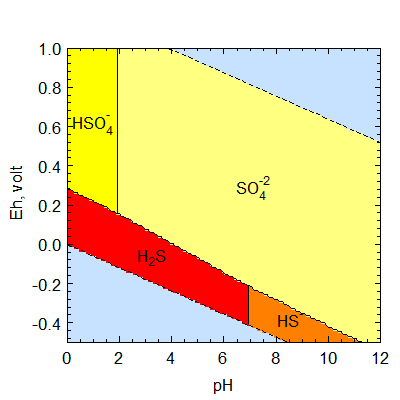
\includegraphics[width=1\linewidth]{anintro_chnosz_files/figure-latex/EhpH_plot-1} \caption[Aqueous sulfur species at 25 °C]{Aqueous sulfur species at 25 °C.}\label{fig:EhpH_plot}
\end{marginfigure}

Now we can calculate the affinities on an Eh-pH grid:

\begin{Shaded}
\begin{Highlighting}[]
\NormalTok{a <-}\StringTok{ }\KeywordTok{affinity}\NormalTok{(}\DataTypeTok{pH =} \KeywordTok{c}\NormalTok{(}\DecValTok{0}\NormalTok{, }\DecValTok{12}\NormalTok{), }\DataTypeTok{Eh =} \KeywordTok{c}\NormalTok{(}\OperatorTok{-}\FloatTok{0.5}\NormalTok{, }\DecValTok{1}\NormalTok{))}
\end{Highlighting}
\end{Shaded}

\subsection{Potential diagrams}\label{potential-diagrams}

Given values of affinity, the {\texttt{diagram()}} function uses the
maximum affinity method to make a potential diagram (i.e.~a Pourbaix
diagram). Areas corresponding to Eh-pH conditions beyond the stability
limits of water are colored slate gray. Another function,
{\texttt{water.lines()}}, is used to draw lines at the water stability
limits:

\begin{Shaded}
\begin{Highlighting}[]
\KeywordTok{diagram}\NormalTok{(a, }\DataTypeTok{fill =} \StringTok{"heat"}\NormalTok{)}
\KeywordTok{water.lines}\NormalTok{(a)}
\end{Highlighting}
\end{Shaded}

Note that the calculation of affinity implies a non-equilibrium
reference state of equal activities of species
(\protect\hyperlink{species-of-interest}{see above}). Generally, then,
{\texttt{diagram()}} gives a \emph{potential diagram} because it shows
regions of maximum affinity. In systems where equilibrium is attainable,
it makes sense to call this a \emph{predominance diagram}, showing
regions of maximum activity.

\begin{marginfigure}
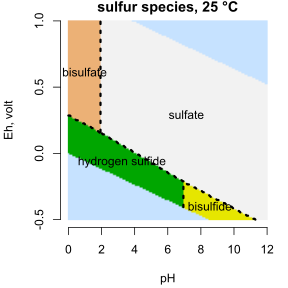
\includegraphics[width=1\linewidth]{anintro_chnosz_files/figure-latex/EhpH_plot_color-1} \caption[The same plot, with different colors and labels]{The same plot, with different colors and labels.}\label{fig:EhpH_plot_color}
\end{marginfigure}

The names of species that can be parsed as chemical formulas are
formatted with subscripts and superscripts; if this is not desired, set
\texttt{format.names\ =\ FALSE}. The default colors for diagrams shown
on the screen use R's \texttt{heat.colors()} palette. Some arguments in
{\texttt{diagram()}} can be used to control the color, labels, and
lines, and title. The \texttt{tplot} argument turns off plot
customizations used in CHNOSZ. Additional arguments are passed to R's
plotting functions; here, we use \texttt{bty} to remove the box around
the plot.

\begin{Shaded}
\begin{Highlighting}[]
\KeywordTok{diagram}\NormalTok{(a, }\DataTypeTok{fill =} \StringTok{"terrain"}\NormalTok{, }\DataTypeTok{lwd =} \DecValTok{3}\NormalTok{, }\DataTypeTok{lty =} \DecValTok{3}\NormalTok{,}
        \DataTypeTok{names =} \KeywordTok{c}\NormalTok{(}\StringTok{"hydrogen sulfide"}\NormalTok{, }\StringTok{"bisulfide"}\NormalTok{, }\StringTok{"bisulfate"}\NormalTok{, }\StringTok{"sulfate"}\NormalTok{),}
        \DataTypeTok{tplot =} \OtherTok{FALSE}\NormalTok{, }\DataTypeTok{main =} \StringTok{"sulfur species, 25 °C"}\NormalTok{, }\DataTypeTok{bty =} \StringTok{"n"}\NormalTok{)}
\end{Highlighting}
\end{Shaded}

Mineral stability diagrams often depict activity ratios, e.g.~log
(\emph{a}Ca+2/\emph{a}H+2), on one or both axes. The variables used for
potential calculations in CHNOSZ include only a single chemical
activity, e.g.~log \emph{a}Ca+2. However, you can set pH = 0 to generate
diagrams that are geometrically equivalent to those calculated using
activity ratios, and use {\texttt{ratlab()}} to make the axes labels for
the ratios. See \href{../demo}{{\texttt{demo(activity\_ratios)}}} for
some examples.

\hypertarget{mosaic-diagrams}{\subsection{Mosaic
diagrams}\label{mosaic-diagrams}}

If sulfur is in the basis species, then we should consider that its
speciation is sensitive to Eh and pH, as shown in the preceding diagram.
Mosaic diagrams, which are often shown for oxide, sulfide, and carbonate
minerals, account for speciation of the basis species. These diagrams
are made by constructing individual diagrams for the possible basis
species. The individual diagrams are then combined, each one
contributing to the final diagram only in the range of stability of the
corresponding basis species.

Let's use {\texttt{mosaic()}} to make a diagram for aqueous species and
minerals in the Cu-S-Cl-H2O system, similar to Figure 5a of
\citet{CPCC17}. To know what aqueous copper chloride complexes are
available in the database, we can use a fuzzy search:

\begin{Shaded}
\begin{Highlighting}[]
\KeywordTok{info}\NormalTok{(}\StringTok{" CuCl"}\NormalTok{)}
\end{Highlighting}
\end{Shaded}

We wish to include chalcocite (Cu2S) in the system. This mineral
undergoes phase transitions; to find out the temperatures of the phase
transitions, we can also use {\texttt{info()}}:

\begin{Shaded}
\begin{Highlighting}[]
\KeywordTok{info}\NormalTok{(}\KeywordTok{info}\NormalTok{(}\StringTok{"chalcocite"}\NormalTok{, }\KeywordTok{c}\NormalTok{(}\StringTok{"cr"}\NormalTok{, }\StringTok{"cr2"}\NormalTok{, }\StringTok{"cr3"}\NormalTok{)))}\OperatorTok{$}\NormalTok{T}
\end{Highlighting}
\end{Shaded}

\begin{verbatim}
## [1]  376  717 1400
\end{verbatim}

Those are temperatures in Kelvin (regardless of the
{\texttt{T.units()}}); at 200 °C we should use the second phase.

Next we define the basis, and set the activities of the H2S and Cl-
basis species. These represent the total activity of S and Cl in the
system, which are distributed among the minerals and aqueous species.
Three minerals and the aqueous copper chloride species are included:

\begin{Shaded}
\begin{Highlighting}[]
\KeywordTok{basis}\NormalTok{(}\KeywordTok{c}\NormalTok{(}\StringTok{"Cu"}\NormalTok{, }\StringTok{"H2S"}\NormalTok{, }\StringTok{"Cl-"}\NormalTok{, }\StringTok{"H2O"}\NormalTok{, }\StringTok{"H+"}\NormalTok{, }\StringTok{"e-"}\NormalTok{))}
\KeywordTok{basis}\NormalTok{(}\StringTok{"H2S"}\NormalTok{, }\OperatorTok{-}\DecValTok{6}\NormalTok{)}
\KeywordTok{basis}\NormalTok{(}\StringTok{"Cl-"}\NormalTok{, }\OperatorTok{-}\FloatTok{0.7}\NormalTok{)}
\KeywordTok{species}\NormalTok{(}\KeywordTok{c}\NormalTok{(}\StringTok{"copper"}\NormalTok{, }\StringTok{"tenorite"}\NormalTok{))}
\KeywordTok{species}\NormalTok{(}\StringTok{"chalcocite"}\NormalTok{, }\StringTok{"cr2"}\NormalTok{)}
\KeywordTok{species}\NormalTok{(}\KeywordTok{c}\NormalTok{(}\StringTok{"CuCl"}\NormalTok{, }\StringTok{"CuCl2-"}\NormalTok{, }\StringTok{"CuCl3-2"}\NormalTok{, }\StringTok{"CuCl+"}\NormalTok{, }\StringTok{"CuCl2"}\NormalTok{, }\StringTok{"CuCl3-"}\NormalTok{, }\StringTok{"CuCl4-2"}\NormalTok{))}
\end{Highlighting}
\end{Shaded}

We use {\texttt{mosaic()}} to generate and combine diagrams for each
candidate basis species (H2S, HS-, HSO4-, or SO4-2) as a function of Eh
and pH. The key argument is \texttt{bases}, which identifies the
candidate basis species, starting with the one in the current basis. The
other arguments, like those of {\texttt{affinity()}}, specify the ranges
of the variables; \texttt{res} indicates the grid resolution to use for
each variable (the default is 128). The first call to
{\texttt{diagram()}} plots the species of interest; the second adds the
predominance fields of the basis species. We turn off the gray coloring
beyond the water stability limits (\texttt{limit.water}) but plot the
red dotted lines using {\texttt{water.lines()}}:

\begin{marginfigure}
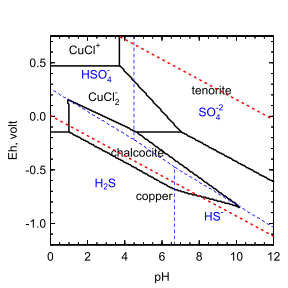
\includegraphics[width=1\linewidth]{anintro_chnosz_files/figure-latex/copper_mosaic-1} \caption[Copper minerals and aqueous complexes with chloride, 200 °C]{Copper minerals and aqueous complexes with chloride, 200 °C.}\label{fig:copper_mosaic}
\end{marginfigure}

\begin{Shaded}
\begin{Highlighting}[]
\NormalTok{T <-}\StringTok{ }\DecValTok{200}
\NormalTok{res <-}\StringTok{ }\DecValTok{200}
\NormalTok{bases <-}\StringTok{ }\KeywordTok{c}\NormalTok{(}\StringTok{"H2S"}\NormalTok{, }\StringTok{"HS-"}\NormalTok{, }\StringTok{"HSO4-"}\NormalTok{, }\StringTok{"SO4-2"}\NormalTok{)}
\NormalTok{m1 <-}\StringTok{ }\KeywordTok{mosaic}\NormalTok{(bases, }\DataTypeTok{blend =} \OtherTok{TRUE}\NormalTok{, }\DataTypeTok{pH =} \KeywordTok{c}\NormalTok{(}\DecValTok{0}\NormalTok{, }\DecValTok{12}\NormalTok{, res), }\DataTypeTok{Eh=}\KeywordTok{c}\NormalTok{(}\OperatorTok{-}\FloatTok{1.2}\NormalTok{, }\FloatTok{0.75}\NormalTok{, res), }\DataTypeTok{T=}\NormalTok{T)}
\KeywordTok{diagram}\NormalTok{(m1}\OperatorTok{$}\NormalTok{A.species, }\DataTypeTok{lwd =} \DecValTok{2}\NormalTok{, }\DataTypeTok{fill =} \OtherTok{NA}\NormalTok{, }\DataTypeTok{limit.water =} \OtherTok{FALSE}\NormalTok{)}
\KeywordTok{diagram}\NormalTok{(m1}\OperatorTok{$}\NormalTok{A.bases, }\DataTypeTok{add =} \OtherTok{TRUE}\NormalTok{, }\DataTypeTok{col =} \StringTok{"blue"}\NormalTok{, }\DataTypeTok{col.names =} \StringTok{"blue"}\NormalTok{, }\DataTypeTok{lty =} \DecValTok{2}\NormalTok{,}
        \DataTypeTok{limit.water =} \OtherTok{FALSE}\NormalTok{)}
\KeywordTok{water.lines}\NormalTok{(m1}\OperatorTok{$}\NormalTok{A.species, }\DataTypeTok{col =} \StringTok{"red"}\NormalTok{, }\DataTypeTok{lwd =} \DecValTok{2}\NormalTok{, }\DataTypeTok{lty =} \DecValTok{3}\NormalTok{)}
\end{Highlighting}
\end{Shaded}

The argument \texttt{blend\ =\ TRUE} is used to combine the diagrams
according to the equilibrium activities of the basis species by
themselves (\protect\hyperlink{equilibration}{see below}). The smooth
transitions between basis species cause the appearance of curved lines
on the plot. Without that argument, the diagrams would be combined using
the dominant basis species, and all of the line segments would be
straight.

 We have seen the effects of speciation of S in the basis species.
However, the choice of other basis species can also affect the diagram.
For instance, we can use H2 or O2 in place of \emph{e}-. To do that,
let's write a function to swap those basis species and make a diagram.
We use R's \texttt{do.call()} to construct the argument list for
{\texttt{mosaic()}}; this way, the name of the \texttt{newvar} argument
to our function indicates the chosen variable.

\begin{Shaded}
\begin{Highlighting}[]
\NormalTok{mosaicfun <-}\StringTok{ }\ControlFlowTok{function}\NormalTok{(newvar, }\DataTypeTok{T =} \DecValTok{200}\NormalTok{) \{}
  \KeywordTok{swap.basis}\NormalTok{(}\StringTok{"e-"}\NormalTok{, }\KeywordTok{names}\NormalTok{(newvar))}
  \ControlFlowTok{if}\NormalTok{ (}\KeywordTok{names}\NormalTok{(newvar) }\OperatorTok{==}\StringTok{ "O2"}\NormalTok{) }\KeywordTok{basis}\NormalTok{(}\StringTok{"O2"}\NormalTok{, }\StringTok{"gas"}\NormalTok{)}
\NormalTok{  mosaicargs <-}\StringTok{ }\KeywordTok{c}\NormalTok{(}\KeywordTok{list}\NormalTok{(bases), }\DataTypeTok{blend=}\OtherTok{TRUE}\NormalTok{, }\DataTypeTok{pH=}\KeywordTok{list}\NormalTok{(}\KeywordTok{c}\NormalTok{(}\OperatorTok{-}\DecValTok{2}\NormalTok{, }\DecValTok{12}\NormalTok{, res)), newvar, }\DataTypeTok{T=}\NormalTok{T)}
\NormalTok{  m1 <-}\StringTok{ }\KeywordTok{do.call}\NormalTok{(mosaic, mosaicargs)}
  \KeywordTok{diagram}\NormalTok{(m1}\OperatorTok{$}\NormalTok{A.species, }\DataTypeTok{lwd =} \DecValTok{2}\NormalTok{, }\DataTypeTok{fill =} \KeywordTok{rev}\NormalTok{(}\KeywordTok{topo.colors}\NormalTok{(}\DecValTok{10}\NormalTok{)),}
          \DataTypeTok{limit.water =} \OtherTok{FALSE}\NormalTok{)}
  \KeywordTok{diagram}\NormalTok{(m1}\OperatorTok{$}\NormalTok{A.bases, }\DataTypeTok{add =} \OtherTok{TRUE}\NormalTok{, }\DataTypeTok{col =} \StringTok{"blue"}\NormalTok{, }\DataTypeTok{col.names =} \StringTok{"blue"}\NormalTok{, }\DataTypeTok{lty =} \DecValTok{3}\NormalTok{,}
          \DataTypeTok{limit.water =} \OtherTok{FALSE}\NormalTok{)}
  \KeywordTok{water.lines}\NormalTok{(m1}\OperatorTok{$}\NormalTok{A.species, }\DataTypeTok{col =} \StringTok{"red"}\NormalTok{, }\DataTypeTok{lwd =} \DecValTok{2}\NormalTok{, }\DataTypeTok{lty =} \DecValTok{3}\NormalTok{)}
  \KeywordTok{swap.basis}\NormalTok{(}\KeywordTok{names}\NormalTok{(newvar), }\StringTok{"e-"}\NormalTok{)}
\NormalTok{\}}
\KeywordTok{par}\NormalTok{(}\DataTypeTok{mfrow =} \KeywordTok{c}\NormalTok{(}\DecValTok{1}\NormalTok{, }\DecValTok{3}\NormalTok{))}
\KeywordTok{mosaicfun}\NormalTok{(}\KeywordTok{list}\NormalTok{(}\DataTypeTok{Eh =} \KeywordTok{c}\NormalTok{(}\OperatorTok{-}\DecValTok{1}\NormalTok{, }\DecValTok{1}\NormalTok{, res)))}
\KeywordTok{mosaicfun}\NormalTok{(}\KeywordTok{list}\NormalTok{(}\DataTypeTok{H2 =} \KeywordTok{c}\NormalTok{(}\OperatorTok{-}\DecValTok{30}\NormalTok{, }\DecValTok{10}\NormalTok{, res)))}
\KeywordTok{mosaicfun}\NormalTok{(}\KeywordTok{list}\NormalTok{(}\DataTypeTok{O2 =} \KeywordTok{c}\NormalTok{(}\OperatorTok{-}\DecValTok{70}\NormalTok{, }\DecValTok{5}\NormalTok{, res)))}
\end{Highlighting}
\end{Shaded}

\begin{figure*}
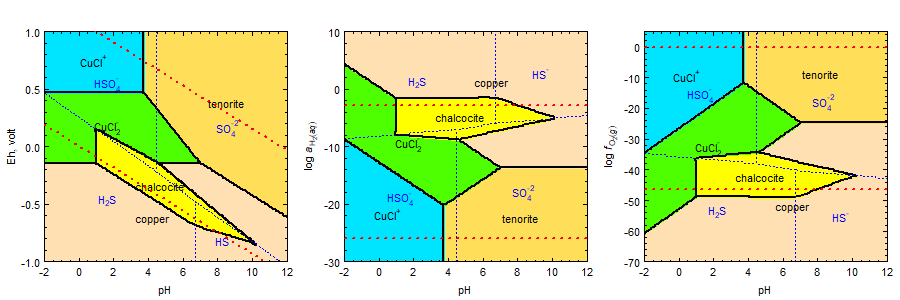
\includegraphics[width=0.85\linewidth]{anintro_chnosz_files/figure-latex/mosaicfun-1} \caption[The same chemical system projected into different sets of basis species]{The same chemical system projected into different sets of basis species.}\label{fig:mosaicfun}
\end{figure*}

\hypertarget{t-p-activity-transects}{\subsection{\texorpdfstring{\emph{T},
\emph{P}, activity
transects}{T, P, activity transects}}\label{t-p-activity-transects}}

Above, we used evenly-spaced grids of chemical activities of basis
species; the ranges of variables were given by two or three values
(minimum, maximum, and optionally resolution). {\texttt{affinity()}} can
also perform calculations along a transect, i.e.~a particular path along
one or more variables. A transect is calculated when there are four or
more values assigned to the variable(s). Let's use this feature to
calculate affinities (negative Gibbs energies) of methanogenesis and
biosynthetic reactions in a hydrothermal system.

Some results of mixing calculations for seawater and vent fluid from the
Rainbow hydrothermal field, calculated using EQ3/6 by \citet{SC10}, are
included in a data file in CHNOSZ. Reading the file with R's
\texttt{read.csv()}, we set \texttt{check.names\ =\ FALSE} to preserve
the \texttt{NH4+} column name (which is not a syntactically valid
variable name):

\begin{Shaded}
\begin{Highlighting}[]
\NormalTok{file <-}\StringTok{ }\KeywordTok{system.file}\NormalTok{(}\StringTok{"extdata/cpetc/SC10_Rainbow.csv"}\NormalTok{, }\DataTypeTok{package =} \StringTok{"CHNOSZ"}\NormalTok{)}
\NormalTok{rb <-}\StringTok{ }\KeywordTok{read.csv}\NormalTok{(file, }\DataTypeTok{check.names =} \OtherTok{FALSE}\NormalTok{)}
\end{Highlighting}
\end{Shaded}

We take a selection of the species from Shock and Canovas (2010) with
activities equal to 10-6; methane is assigned an activity of 10-3. We
will write the synthesis reactions of organic species in terms of these
basis species:

\begin{marginfigure}
The constant activity of methane is a simplification of the calculation
reported by Shock and Canovas (2010). The code here could be expanded to
vary the activity of methane.
\end{marginfigure}

\begin{Shaded}
\begin{Highlighting}[]
\KeywordTok{basis}\NormalTok{(}\KeywordTok{c}\NormalTok{(}\StringTok{"CO2"}\NormalTok{, }\StringTok{"H2"}\NormalTok{, }\StringTok{"NH4+"}\NormalTok{, }\StringTok{"H2O"}\NormalTok{, }\StringTok{"H2S"}\NormalTok{, }\StringTok{"H+"}\NormalTok{))}
\KeywordTok{species}\NormalTok{(}\StringTok{"CH4"}\NormalTok{, }\OperatorTok{-}\DecValTok{3}\NormalTok{)}
\KeywordTok{species}\NormalTok{(}\KeywordTok{c}\NormalTok{(}\StringTok{"adenine"}\NormalTok{, }\StringTok{"cytosine"}\NormalTok{, }\StringTok{"aspartic acid"}\NormalTok{, }\StringTok{"deoxyribose"}\NormalTok{,}
          \StringTok{"methane"}\NormalTok{, }\StringTok{"leucine"}\NormalTok{, }\StringTok{"tryptophan"}\NormalTok{, }\StringTok{"n-nonanoic acid"}\NormalTok{), }\OperatorTok{-}\DecValTok{6}\NormalTok{)}
\end{Highlighting}
\end{Shaded}

Now we can calculate affinities along the transect of changing
temperature and activities of five basis species. Each variable is given
as a named argument; \texttt{NH4+} must be quoted.

\begin{marginfigure}
A shorter expression would use R's \texttt{do.call()} to construct the
function call:
\texttt{do.call(}{\texttt{affinity}}\texttt{,\ as.list(rb))}.
\end{marginfigure}\begin{marginfigure}
The target of the conversion is \texttt{G}, or free energy, from
\texttt{logK}. That conversion requires temperature in Kelvin, which is
obtained by conversion from °C. We finish with a negation (affinity is
negative Gibbs energy) and scaling from cal to kcal.
\end{marginfigure}

Using R's \texttt{lapply()} to run {\texttt{convert()}} for each
species, we convert the affinity from dimensionless values
(\emph{A}/(2.303\emph{RT})) to cal/mol, then kcal/mol.

\begin{Shaded}
\begin{Highlighting}[]
\NormalTok{a <-}\StringTok{ }\KeywordTok{affinity}\NormalTok{(}\DataTypeTok{T =}\NormalTok{ rb}\OperatorTok{$}\NormalTok{T, }\DataTypeTok{CO2 =}\NormalTok{ rb}\OperatorTok{$}\NormalTok{CO2, }\DataTypeTok{H2 =}\NormalTok{ rb}\OperatorTok{$}\NormalTok{H2,}
              \StringTok{`}\DataTypeTok{NH4+}\StringTok{`}\NormalTok{ =}\StringTok{ }\NormalTok{rb}\OperatorTok{$}\StringTok{`}\DataTypeTok{NH4+}\StringTok{`}\NormalTok{, }\DataTypeTok{H2S =}\NormalTok{ rb}\OperatorTok{$}\NormalTok{H2S, }\DataTypeTok{pH =}\NormalTok{ rb}\OperatorTok{$}\NormalTok{pH)}
\NormalTok{T <-}\StringTok{ }\KeywordTok{convert}\NormalTok{(a}\OperatorTok{$}\NormalTok{vals[[}\DecValTok{1}\NormalTok{]], }\StringTok{"K"}\NormalTok{)}
\NormalTok{a}\OperatorTok{$}\NormalTok{values <-}\StringTok{ }\KeywordTok{lapply}\NormalTok{(a}\OperatorTok{$}\NormalTok{values, convert, }\StringTok{"G"}\NormalTok{, T)}
\NormalTok{a}\OperatorTok{$}\NormalTok{values <-}\StringTok{ }\KeywordTok{lapply}\NormalTok{(a}\OperatorTok{$}\NormalTok{values, }\StringTok{`}\DataTypeTok{*}\StringTok{`}\NormalTok{, }\OperatorTok{-}\FloatTok{0.001}\NormalTok{)}
\end{Highlighting}
\end{Shaded}

\begin{marginfigure}
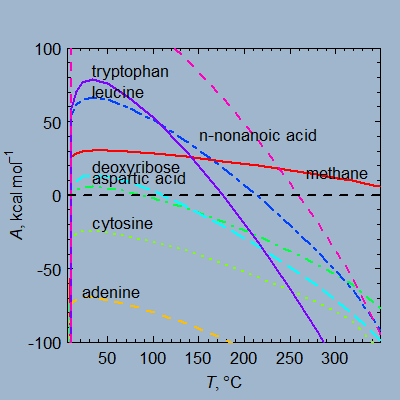
\includegraphics[width=1\linewidth]{anintro_chnosz_files/figure-latex/rainbow_diagram-1} \caption[Affinities of organic synthesis in a hydrothermal system, after Shock and Canovas (2010)]{Affinities of organic synthesis in a hydrothermal system, after Shock and Canovas (2010).}\label{fig:rainbow_diagram}
\end{marginfigure}

Finally, we use {\texttt{diagram()}} to plot the results. Although only
temperature is shown on the \emph{x} axis, pH and the activities of CO2,
H2, NH4+, and H2S are also varied according to the data in \texttt{rb}.
By default, {\texttt{diagram()}} attempts to scale the affinities by
dividing by the reaction coefficients of a shared basis species (in this
case, CO2). To override that behavior, we set \texttt{balance\ =\ 1} to
plot the affinities of the formation reactions as written (per mole of
the product species).

\begin{Shaded}
\begin{Highlighting}[]
\KeywordTok{diagram}\NormalTok{(a, }\DataTypeTok{balance =} \DecValTok{1}\NormalTok{, }\DataTypeTok{ylim =} \KeywordTok{c}\NormalTok{(}\OperatorTok{-}\DecValTok{100}\NormalTok{, }\DecValTok{100}\NormalTok{), }\DataTypeTok{ylab =} \KeywordTok{axis.label}\NormalTok{(}\StringTok{"A"}\NormalTok{, }\DataTypeTok{prefix=}\StringTok{"k"}\NormalTok{),}
        \DataTypeTok{col =} \KeywordTok{rainbow}\NormalTok{(}\DecValTok{8}\NormalTok{), }\DataTypeTok{lwd =} \DecValTok{2}\NormalTok{, }\DataTypeTok{bg =} \StringTok{"slategray3"}\NormalTok{)}
\KeywordTok{abline}\NormalTok{(}\DataTypeTok{h =} \DecValTok{0}\NormalTok{, }\DataTypeTok{lty =} \DecValTok{2}\NormalTok{, }\DataTypeTok{lwd =} \DecValTok{2}\NormalTok{)}
\end{Highlighting}
\end{Shaded}

When making line plots, {\texttt{diagram()}} automatically places the
labels near the lines. The additional arguments \texttt{adj} and
\texttt{dy} can be used to fine-tune the positions of the labels (they
are used in a couple of examples below). If labeling of the lines is not
desired, add e.g. \texttt{legend.x\ =\ "topright"} to make a legend
instead, or \texttt{names\ =\ NULL} to prevent any plotting of the
names.

\subsection{Buffers}\label{buffers}

There is one other feature of {\texttt{affinity()}} that can be
mentioned here. Can we go the other direction: calculate the activities
of basis species from the activities of the species of interest? This
question relates to the concept of chemical activity buffers. In CHNOSZ
there are two ways to perform buffer calculations:

\begin{enumerate}
\def\labelenumi{\arabic{enumi}.}
\tightlist
\item
  Assign the name of a buffer (listed in \texttt{thermo\$buffer}) to the
  basis species:
\end{enumerate}

\begin{itemize}
\tightlist
\item
  more versatile (multiple activities can be buffered, e.g.~both S2 and
  O2 by pyrite-pyrrhotite-magnetite);
\item
  the buffers are active in calculations of affinity of other species;
\item
  use {\texttt{mod.buffer()}} to change or add buffers in
  \texttt{thermo\$buffer};
\item
  \href{../demo}{{\texttt{demo(buffer)}}} uses it for mineral buffers
  (solid lines).
\end{itemize}

\begin{enumerate}
\def\labelenumi{\arabic{enumi}.}
\setcounter{enumi}{1}
\tightlist
\item
  Use the \texttt{what} argument of {\texttt{diagram()}} to solve for
  the activity of the indicated basis species:
\end{enumerate}

\begin{itemize}
\tightlist
\item
  more convenient (the buffers come from the currently defined species
  of interest), but only a single basis species can be buffered, and
  it's not used in the calculation of affinity;
\item
  \href{../demo}{{\texttt{demo(buffer)}}} uses it for aqueous organic
  species as buffers (dotted and dashed lines).
\end{itemize}

As an example of method 1, let's look at the pyrite-pyrrhotite-magnetite
(PPM) buffer at 300 °C.

\begin{marginfigure}
For other examples, see {\texttt{?buffer}} and
\href{../demo}{{\texttt{demo(protbuff)}}} (hypothetical buffer made of
proteins).
\end{marginfigure}

Without the buffer, the basis species have default activities of zero.
Under these conditions, the minerals are not in equilibrium, as shown by
their different affinities of formation:

\begin{Shaded}
\begin{Highlighting}[]
\KeywordTok{basis}\NormalTok{(}\KeywordTok{c}\NormalTok{(}\StringTok{"FeS2"}\NormalTok{, }\StringTok{"H2S"}\NormalTok{, }\StringTok{"O2"}\NormalTok{, }\StringTok{"H2O"}\NormalTok{))}
\KeywordTok{species}\NormalTok{(}\KeywordTok{c}\NormalTok{(}\StringTok{"pyrite"}\NormalTok{, }\StringTok{"magnetite"}\NormalTok{))}
\KeywordTok{species}\NormalTok{(}\StringTok{"pyrrhotite"}\NormalTok{, }\StringTok{"cr2"}\NormalTok{)}
\end{Highlighting}
\end{Shaded}

\begin{marginfigure}
The affinity of formation of pyrite happens to be zero because it is
identical to one of the selected basis species.
\end{marginfigure}

\begin{Shaded}
\begin{Highlighting}[]
\KeywordTok{unlist}\NormalTok{(}\KeywordTok{affinity}\NormalTok{(}\DataTypeTok{T =} \DecValTok{300}\NormalTok{, }\DataTypeTok{P =} \DecValTok{100}\NormalTok{)}\OperatorTok{$}\NormalTok{values)}
\end{Highlighting}
\end{Shaded}

\begin{verbatim}
##     2113     2081     2118 
##   0.0000 -50.6501 -20.6134
\end{verbatim}

We use {\texttt{mod.buffer()}} to choose the \texttt{cr2} phase of
pyrrhotite, which is stable at this temperature
(\protect\hyperlink{mosaic-diagrams}{see above} for how to get this
information for minerals with phase transitions). Then, we set up H2S
and O2 to be buffered by PPM, and inspect their buffered activities:

\begin{Shaded}
\begin{Highlighting}[]
\KeywordTok{mod.buffer}\NormalTok{(}\StringTok{"PPM"}\NormalTok{, }\StringTok{"pyrrhotite"}\NormalTok{, }\StringTok{"cr2"}\NormalTok{)}
\end{Highlighting}
\end{Shaded}

\begin{Shaded}
\begin{Highlighting}[]
\KeywordTok{basis}\NormalTok{(}\KeywordTok{c}\NormalTok{(}\StringTok{"H2S"}\NormalTok{, }\StringTok{"O2"}\NormalTok{), }\KeywordTok{c}\NormalTok{(}\StringTok{"PPM"}\NormalTok{, }\StringTok{"PPM"}\NormalTok{))}
\end{Highlighting}
\end{Shaded}

\begin{Shaded}
\begin{Highlighting}[]
\KeywordTok{unlist}\NormalTok{(}\KeywordTok{affinity}\NormalTok{(}\DataTypeTok{T =} \DecValTok{300}\NormalTok{, }\DataTypeTok{P =} \DecValTok{100}\NormalTok{, }\DataTypeTok{return.buffer =} \OtherTok{TRUE}\NormalTok{)[}\DecValTok{1}\OperatorTok{:}\DecValTok{3}\NormalTok{])}
\end{Highlighting}
\end{Shaded}

\begin{verbatim}
##       H2S        O2      FeS2 
##  -2.35581 -36.51522   0.00000
\end{verbatim}

\begin{marginfigure}
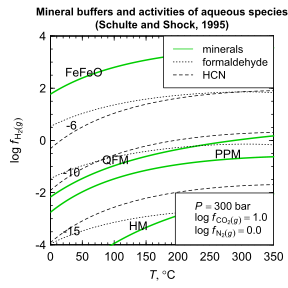
\includegraphics[width=1\linewidth]{anintro_chnosz_files/figure-latex/demo_buffer_noecho-1} \caption[Values of log<i>f</i><sub>H<sub>2</sub></sub> corresponding to mineral buffers or to given activities of aqueous species]{Values of log<i>f</i><sub>H<sub>2</sub></sub> corresponding to mineral buffers or to given activities of aqueous species.}\label{fig:demo_buffer_noecho}
\end{marginfigure}

Et voilÃ~! We have found log\emph{a}H2S and logfO2 that are compatible
with the coexistence of the three minerals. Under these conditions, the
affinities of formation reactions of the minerals in the buffer are all
equal to zero:

\begin{Shaded}
\begin{Highlighting}[]
\KeywordTok{unlist}\NormalTok{(}\KeywordTok{affinity}\NormalTok{(}\DataTypeTok{T =} \DecValTok{300}\NormalTok{, }\DataTypeTok{P =} \DecValTok{100}\NormalTok{)}\OperatorTok{$}\NormalTok{values)}
\NormalTok{## 2031 1999 2036 }
\NormalTok{##    0    0    0}
\end{Highlighting}
\end{Shaded}

Another example, based on Figure 6 of \citet{SS95}, is given in
\href{../demo}{{\texttt{demo(buffer)}}}. Here, values of log\emph{f}H2
buffered by minerals or set by equilibrium with given activities of
aqueous species are calculated using the two methods:

\begin{Shaded}
\begin{Highlighting}[]
\KeywordTok{demo}\NormalTok{(buffer)}
\end{Highlighting}
\end{Shaded}

\hypertarget{equilibration}{\section{Equilibration}\label{equilibration}}

Above we considered this kind of question: for equal activities of
species, what are the affinities of their formation reactions from basis
species? Turning the question around, we would like to know: for equal
affinities, what are the activities of species? This is the question of
equilibration.

Before presenting some examples, it is helpful to know about the
limitations of the functions. CHNOSZ does not take account of all
possible reactions in the speciation of a system. Instead, it assumes
that the total activity of species in the system is set by the activity
of \emph{one} basis species.

\begin{marginfigure}
When activity coefficients are assumed to be zero, activities are equal
to concentration and we can refer to ``total activity''. If the ionic
strength is specified, {\texttt{nonideal()}}
(\protect\hyperlink{activity-coefficients}{see below}) can be used to
calculate activity coefficients.
\end{marginfigure}

This balanced, or conserved, basis species must be present (with a
positive or negative coefficient) in the formation reactions of all
species considered.

For a given total activity of the balanced basis species, activities of
the species can be found such that the affinities of the formation
reactions are all equal. This is an example of metastable equilibrium.
With additional constraints, the affinities of the formation reactions
are not only equal to each other, but equal to zero. This is total
equilibrium. An example of total equilibrium was given above for the PPM
buffer. In contrast, models for systems of organic and biomolecules
often involve metastable equilibrium constraints.

\subsection{Getting from affinity to
equilibrium}\label{getting-from-affinity-to-equilibrium}

The {\texttt{equilibrate()}} function in CHNOSZ automatically chooses
between two methods for calculating equilibrium.

\begin{marginfigure}
For more information, see the vignette
\href{equilibrium.pdf}{{\emph{Equilibrium in CHNOSZ}}}.
\end{marginfigure}

The method based on the Boltzmann equation is fast, but is applicable
only to systems where the coefficient on the balanced basis species in
each of the formation reactions is one. The reaction-matrix method is
slower, but can be applied to systems were the balanced basis species
has reaction coefficients other than one.

\begin{marginfigure}
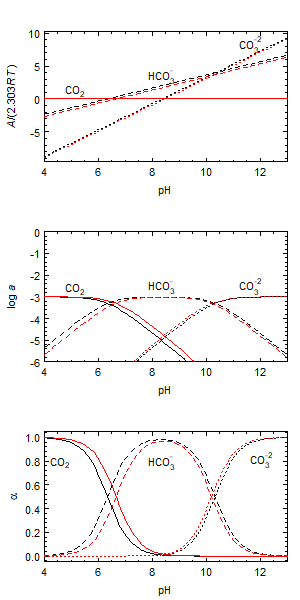
\includegraphics[width=1\linewidth]{anintro_chnosz_files/figure-latex/bjerrum_diagram-1} \caption[Three views of carbonate speciation]{Three views of carbonate speciation: affinity, activity, degree of formation.}\label{fig:bjerrum_diagram}
\end{marginfigure}

The distribution of aqueous carbonate species as a function of pH (a
type of Bjerrum plot) is a classic example of an equilibrium
calculation. We can begin by plotting the affinities of formation, for
equal activities of the species, calculated at 25 °C and 150 °C. Here,
CO2 is in the basis, so it has zero affinity, which is greater than the
affinities of HCO3- and CO3-2 at low pH. To avoid overplotting the
lines, we offset the species labels in the \emph{y} direction using the
\texttt{dy} argument:

\begin{Shaded}
\begin{Highlighting}[]
\KeywordTok{par}\NormalTok{(}\DataTypeTok{mfrow =} \KeywordTok{c}\NormalTok{(}\DecValTok{3}\NormalTok{, }\DecValTok{1}\NormalTok{))}
\KeywordTok{basis}\NormalTok{(}\StringTok{"CHNOS+"}\NormalTok{)}
\KeywordTok{species}\NormalTok{(}\KeywordTok{c}\NormalTok{(}\StringTok{"CO2"}\NormalTok{, }\StringTok{"HCO3-"}\NormalTok{, }\StringTok{"CO3-2"}\NormalTok{))}
\NormalTok{a25 <-}\StringTok{ }\KeywordTok{affinity}\NormalTok{(}\DataTypeTok{pH =} \KeywordTok{c}\NormalTok{(}\DecValTok{4}\NormalTok{, }\DecValTok{13}\NormalTok{))}
\NormalTok{a150 <-}\StringTok{ }\KeywordTok{affinity}\NormalTok{(}\DataTypeTok{pH =} \KeywordTok{c}\NormalTok{(}\DecValTok{4}\NormalTok{, }\DecValTok{13}\NormalTok{), }\DataTypeTok{T =} \DecValTok{150}\NormalTok{)}
\KeywordTok{diagram}\NormalTok{(a25, }\DataTypeTok{dy =} \FloatTok{0.4}\NormalTok{)}
\KeywordTok{diagram}\NormalTok{(a150, }\DataTypeTok{add =} \OtherTok{TRUE}\NormalTok{, }\DataTypeTok{col =} \StringTok{"red"}\NormalTok{)}
\end{Highlighting}
\end{Shaded}

Now we use {\texttt{equilibrate()}} to calculate the activities of
species. Our balancing constraint is that the total activity of C is
10-3. This shows a hypothetical metastable equilibrium; we know that for
true equilibrium the total activity of C is affected by pH.

\begin{Shaded}
\begin{Highlighting}[]
\NormalTok{e25 <-}\StringTok{ }\KeywordTok{equilibrate}\NormalTok{(a25, }\DataTypeTok{loga.balance =} \OperatorTok{-}\DecValTok{3}\NormalTok{)}
\NormalTok{e150 <-}\StringTok{ }\KeywordTok{equilibrate}\NormalTok{(a150, }\DataTypeTok{loga.balance =} \OperatorTok{-}\DecValTok{3}\NormalTok{)}
\KeywordTok{diagram}\NormalTok{(e25, }\DataTypeTok{ylim =} \KeywordTok{c}\NormalTok{(}\OperatorTok{-}\DecValTok{6}\NormalTok{, }\DecValTok{0}\NormalTok{), }\DataTypeTok{dy =} \FloatTok{0.15}\NormalTok{)}
\KeywordTok{diagram}\NormalTok{(e150, }\DataTypeTok{add =} \OtherTok{TRUE}\NormalTok{, }\DataTypeTok{col =} \StringTok{"red"}\NormalTok{)}
\end{Highlighting}
\end{Shaded}

To display the species distribution, or degree of formation, add
\texttt{alpha\ =\ TRUE} to the argument list:

\begin{Shaded}
\begin{Highlighting}[]
\KeywordTok{diagram}\NormalTok{(e25, }\DataTypeTok{alpha =} \OtherTok{TRUE}\NormalTok{, }\DataTypeTok{dy =} \OperatorTok{-}\FloatTok{0.25}\NormalTok{)}
\KeywordTok{diagram}\NormalTok{(e150, }\DataTypeTok{alpha =} \OtherTok{TRUE}\NormalTok{, }\DataTypeTok{add =} \OtherTok{TRUE}\NormalTok{, }\DataTypeTok{col =} \StringTok{"red"}\NormalTok{)}
\end{Highlighting}
\end{Shaded}

The possible reactions between species are all balanced on 1 C.
Therefore, although pH alters the total activity of C, in a system with
ideal mixing the total activity of C doesn't affect the relative
activities of these species.

\begin{marginfigure}
See \href{../demo}{{\texttt{demo(solubility)}}} for calculations of the
total activity of C in this ideal system; uncomment a line in the demo
to run calculations for CO2 instead of calcite.
\end{marginfigure}

\subsection{Groups of species}\label{groups-of-species}

Sometimes it is helpful to look at the summed activities of species as
groups on species distribution diagrams. The \texttt{groups} argument of
{\texttt{diagram()}} can be used to sum the activities of species.

To demonstrate this feature, let's consider the distribution of carbon
among organic and inorganic species in the hydrothermal mixing scenario
described by \citet{SS98}. First we define the basis and add two
inorganic species. The \texttt{index.return\ =\ TRUE} argument tells
{\texttt{info()}} to return the index (number) of the species in the
current species definition; these indices are saved for use below:

\begin{Shaded}
\begin{Highlighting}[]
\KeywordTok{basis}\NormalTok{(}\StringTok{"CHNOS+"}\NormalTok{)}
\NormalTok{ii <-}\StringTok{ }\KeywordTok{species}\NormalTok{(}\KeywordTok{c}\NormalTok{(}\StringTok{"CO2"}\NormalTok{, }\StringTok{"HCO3-"}\NormalTok{), }\DataTypeTok{index.return =} \OtherTok{TRUE}\NormalTok{)}
\end{Highlighting}
\end{Shaded}

Next, we add each group of organic species: C1--C8 alcohols, C3--C8
ketones, C2--C12 carboxylic acids and their corresponding anions, and
C2--C8 alkenes. To do this, we provide {\texttt{info()}} with a set of
\texttt{ispecies} values that identify these species. In the database,
the species in each group are ordered by carbon number, so we construct
a sequence from the starting to ending \texttt{ispecies} for each group
using R's \texttt{seq()} function, wrapped by the \texttt{seq2()}
function we write here to make the code shorter:

\begin{Shaded}
\begin{Highlighting}[]
\NormalTok{seq2 <-}\StringTok{ }\ControlFlowTok{function}\NormalTok{(x) }\KeywordTok{seq}\NormalTok{(x[}\DecValTok{1}\NormalTok{], x[}\DecValTok{2}\NormalTok{])}
\NormalTok{ia <-}\StringTok{ }\KeywordTok{species}\NormalTok{(}\KeywordTok{seq2}\NormalTok{(}\KeywordTok{info}\NormalTok{(}\KeywordTok{c}\NormalTok{(}\StringTok{"methanol"}\NormalTok{, }\StringTok{"octanol"}\NormalTok{))), }\DataTypeTok{index.return =} \OtherTok{TRUE}\NormalTok{)}
\NormalTok{ik <-}\StringTok{ }\KeywordTok{species}\NormalTok{(}\KeywordTok{seq2}\NormalTok{(}\KeywordTok{info}\NormalTok{(}\KeywordTok{c}\NormalTok{(}\StringTok{"acetone"}\NormalTok{, }\StringTok{"2-octanone"}\NormalTok{))), }\DataTypeTok{index.return =} \OtherTok{TRUE}\NormalTok{)}
\NormalTok{ic <-}\StringTok{ }\KeywordTok{species}\NormalTok{(}\KeywordTok{seq2}\NormalTok{(}\KeywordTok{info}\NormalTok{(}\KeywordTok{c}\NormalTok{(}\StringTok{"acetic acid"}\NormalTok{,}\StringTok{"n-dodecanoic acid"}\NormalTok{))),}\DataTypeTok{index.return=}\OtherTok{TRUE}\NormalTok{)}
\NormalTok{ica <-}\StringTok{ }\KeywordTok{species}\NormalTok{(}\KeywordTok{seq2}\NormalTok{(}\KeywordTok{info}\NormalTok{(}\KeywordTok{c}\NormalTok{(}\StringTok{"acetate"}\NormalTok{, }\StringTok{"n-dodecanoate"}\NormalTok{))), }\DataTypeTok{index.return =} \OtherTok{TRUE}\NormalTok{)}
\NormalTok{ie <-}\StringTok{ }\KeywordTok{species}\NormalTok{(}\KeywordTok{seq2}\NormalTok{(}\KeywordTok{info}\NormalTok{(}\KeywordTok{c}\NormalTok{(}\StringTok{"ethylene"}\NormalTok{, }\StringTok{"octene"}\NormalTok{))), }\DataTypeTok{index.return =} \OtherTok{TRUE}\NormalTok{)}
\end{Highlighting}
\end{Shaded}

Now we read two data files that contain values of logfO2 and pH as a
function of temperature, digitized from Figure 5 of Shock and Schulte
(1998).

\begin{marginfigure}
The specific values are for calculations with vent fluids initially set
by the fayalite-magnetite-quartz buffer minus 1/2 log\emph{f}O2 (FMQ -
1/2).
\end{marginfigure}

These values were calculated using a speciation and mixing model that is
not available in CHNOSZ; however, we can use these intermediate values
as input to the ``downstream'' calculations that are available in
CHNOSZ. Because of the noise introduced by digitization of the figure,
we smooth the data using R's \texttt{smooth.spline()}; the lower
\emph{T} limit reflects the absence of data below this temperature in
the figure for log\emph{f}O2.

\begin{Shaded}
\begin{Highlighting}[]
\NormalTok{O2dat <-}\StringTok{ }\KeywordTok{read.csv}\NormalTok{(}\KeywordTok{system.file}\NormalTok{(}
  \StringTok{"extdata/cpetc/SS98_Fig5a.csv"}\NormalTok{, }\DataTypeTok{package =} \StringTok{"CHNOSZ"}\NormalTok{))}
\NormalTok{pHdat <-}\StringTok{ }\KeywordTok{read.csv}\NormalTok{(}\KeywordTok{system.file}\NormalTok{(}
  \StringTok{"extdata/cpetc/SS98_Fig5b.csv"}\NormalTok{, }\DataTypeTok{package =} \StringTok{"CHNOSZ"}\NormalTok{))}
\NormalTok{T <-}\StringTok{ }\KeywordTok{seq}\NormalTok{(}\DecValTok{8}\NormalTok{, }\DecValTok{350}\NormalTok{)}
\NormalTok{O2 <-}\StringTok{ }\KeywordTok{predict}\NormalTok{(}\KeywordTok{smooth.spline}\NormalTok{(O2dat}\OperatorTok{$}\NormalTok{T, O2dat}\OperatorTok{$}\NormalTok{logfO2), T)}\OperatorTok{$}\NormalTok{y}
\NormalTok{pH <-}\StringTok{ }\KeywordTok{predict}\NormalTok{(}\KeywordTok{smooth.spline}\NormalTok{(pHdat}\OperatorTok{$}\NormalTok{T, pHdat}\OperatorTok{$}\NormalTok{pH), T)}\OperatorTok{$}\NormalTok{y}
\end{Highlighting}
\end{Shaded}

We are ready to calculate affinities and equilibrium activities of the
species. This calculation utilizes the transect mode of
{\texttt{affinity()}} (\protect\hyperlink{t-p-activity-transects}{see
above}). The call to {\texttt{equilibrate()}} runs with the default
balance (in this case, CO2), with a log activity set to -2.5.

\begin{marginfigure}
Actually, the total concentration of carbon depends on the mixing ratio,
ranging from about 10-2.2 (seawater) to 10-2.6 (vent fluid). A setting
to vary the activity of the balanced basis species is not yet
implemented in CHNOSZ, so a single value is used here.
\end{marginfigure}

\begin{Shaded}
\begin{Highlighting}[]
\NormalTok{a <-}\StringTok{ }\KeywordTok{affinity}\NormalTok{(}\DataTypeTok{T =}\NormalTok{ T, }\DataTypeTok{O2 =}\NormalTok{ O2, }\DataTypeTok{pH =}\NormalTok{ pH)}
\NormalTok{e <-}\StringTok{ }\KeywordTok{equilibrate}\NormalTok{(a, }\DataTypeTok{loga.balance =} \OperatorTok{-}\FloatTok{2.5}\NormalTok{)}
\end{Highlighting}
\end{Shaded}

At last we come to the diagram. The groups are identified by the current
species numbers in a list; the elements of the list are given names that
will appear on the diagram. When summing the activities of species in
the groups, each activity is multiplied first by the balance coefficient
on that species. Therefore, the total activity is that of a basis
species (or of an element that is present only in that basis species,
like carbon in this example).

\begin{Shaded}
\begin{Highlighting}[]
\KeywordTok{par}\NormalTok{(}\DataTypeTok{mfrow =} \KeywordTok{c}\NormalTok{(}\DecValTok{1}\NormalTok{, }\DecValTok{3}\NormalTok{))}
\NormalTok{groups <-}\StringTok{ }\KeywordTok{list}\NormalTok{(}\DataTypeTok{inorganic =}\NormalTok{ ii, }\DataTypeTok{alcohols =}\NormalTok{ ia, }\DataTypeTok{ketones =}\NormalTok{ ik,}
               \StringTok{`}\DataTypeTok{carboxylic acids}\StringTok{`}\NormalTok{ =}\StringTok{ }\KeywordTok{c}\NormalTok{(ic, ica), }\DataTypeTok{alkenes =}\NormalTok{ ie)}
\KeywordTok{diagram}\NormalTok{(e, }\DataTypeTok{alpha =} \OtherTok{TRUE}\NormalTok{, }\DataTypeTok{groups =}\NormalTok{ groups, }\DataTypeTok{col =} \DecValTok{1}\OperatorTok{:}\DecValTok{5}\NormalTok{)}
\end{Highlighting}
\end{Shaded}

That makes a diagram that is similar to Figure 6b of Shock and Schulte
(1998).

\begin{marginfigure}
Some differences from the original diagrams could be caused by the
sensitivity of the calculations to log\emph{f}O2, for which the values
we use here may carry artifacts introduced by digitization of their
plot.
\end{marginfigure}

It is also possible to plot the distribution of species within
individual groups, such as alcohols and ketones. We do this by setting
the names and line types for the \emph{other} species to values that
prevent them from being plotted:

\begin{Shaded}
\begin{Highlighting}[]
\CommentTok{# plot only alcohols}
\NormalTok{names <-}\StringTok{ }\KeywordTok{within}\NormalTok{(}\KeywordTok{species}\NormalTok{(), name[}\OperatorTok{-}\NormalTok{ia] <-}\StringTok{ ""}\NormalTok{)}\OperatorTok{$}\NormalTok{name}
\NormalTok{lty <-}\StringTok{ }\KeywordTok{ifelse}\NormalTok{(names }\OperatorTok{==}\StringTok{ ""}\NormalTok{, }\DecValTok{0}\NormalTok{, }\DecValTok{1}\NormalTok{)}
\KeywordTok{diagram}\NormalTok{(e, }\DataTypeTok{alpha =} \OtherTok{TRUE}\NormalTok{, }\DataTypeTok{ylim =} \KeywordTok{c}\NormalTok{(}\DecValTok{0}\NormalTok{, }\FloatTok{0.32}\NormalTok{), }\DataTypeTok{lty =}\NormalTok{ lty, }\DataTypeTok{names =}\NormalTok{ names)}
\CommentTok{# plot only ketones}
\NormalTok{names <-}\StringTok{ }\KeywordTok{within}\NormalTok{(}\KeywordTok{species}\NormalTok{(), name[}\OperatorTok{-}\NormalTok{ik] <-}\StringTok{ ""}\NormalTok{)}\OperatorTok{$}\NormalTok{name}
\NormalTok{lty <-}\StringTok{ }\KeywordTok{ifelse}\NormalTok{(names }\OperatorTok{==}\StringTok{ ""}\NormalTok{, }\DecValTok{0}\NormalTok{, }\DecValTok{1}\NormalTok{)}
\KeywordTok{diagram}\NormalTok{(e, }\DataTypeTok{alpha =} \OtherTok{TRUE}\NormalTok{, }\DataTypeTok{ylim =} \KeywordTok{c}\NormalTok{(}\DecValTok{0}\NormalTok{, }\FloatTok{0.16}\NormalTok{), }\DataTypeTok{lty =}\NormalTok{ lty, }\DataTypeTok{names =}\NormalTok{ names)}
\end{Highlighting}
\end{Shaded}

\begin{figure*}
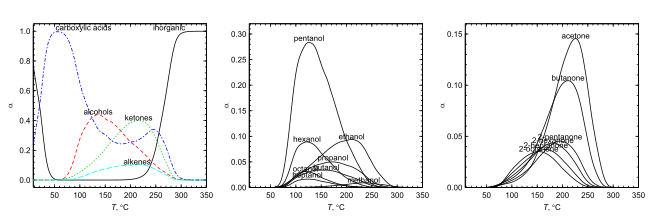
\includegraphics[width=0.85\linewidth]{anintro_chnosz_files/figure-latex/groups_diagram-1} \caption[Distribution of inorganic and groups of organic species (left plot) and of alcohols and ketones (middle and right plots) as a function of <i>T</i>, pH, and log<i>f</i><sub>O<sub>2</sub></sub>]{Distribution of inorganic and groups of organic species (left plot) and of alcohols and ketones (middle and right plots) as a function of <i>T</i>, pH, and log<i>f</i><sub>O<sub>2</sub></sub>.}\label{fig:groups_diagram}
\end{figure*}

\subsection{Balancing differently}\label{balancing-differently}

How about the choice between balancing constraints? Be default,
{\texttt{equilibrate()}} and {\texttt{diagram()}} balance reactions on
the first basis species that is present in each of the species of
interest. Let's look at some amino acids in a hypothetical metastable
equilibrium. This calculation is loosely based on one described by
\citet{Sho90b} for five amino acids. Here we include 20 proteinogenic
amino acids, whose names are returned by {\texttt{aminoacids("")}}. We
use {\texttt{ZC.col()}} to generate colors based on the average
oxidation state of carbon of the amino acids (red and blue for
relatively reduced and oxidized).

\begin{Shaded}
\begin{Highlighting}[]
\KeywordTok{basis}\NormalTok{(}\StringTok{"CHNOS"}\NormalTok{)}
\KeywordTok{basis}\NormalTok{(}\StringTok{"CO2"}\NormalTok{, }\StringTok{"gas"}\NormalTok{)}
\KeywordTok{swap.basis}\NormalTok{(}\StringTok{"NH3"}\NormalTok{, }\StringTok{"N2"}\NormalTok{)}
\KeywordTok{species}\NormalTok{(}\KeywordTok{aminoacids}\NormalTok{(}\StringTok{""}\NormalTok{))}
\NormalTok{a <-}\StringTok{ }\KeywordTok{affinity}\NormalTok{(}\DataTypeTok{O2 =} \KeywordTok{c}\NormalTok{(}\OperatorTok{-}\DecValTok{50}\NormalTok{, }\OperatorTok{-}\DecValTok{25}\NormalTok{, }\DecValTok{200}\NormalTok{), }\DataTypeTok{CO2 =} \KeywordTok{c}\NormalTok{(}\OperatorTok{-}\DecValTok{10}\NormalTok{, }\DecValTok{15}\NormalTok{, }\DecValTok{200}\NormalTok{), }\DataTypeTok{T =} \DecValTok{250}\NormalTok{, }\DataTypeTok{P =} \DecValTok{265}\NormalTok{)}
\NormalTok{aa.ZC <-}\StringTok{ }\KeywordTok{ZC}\NormalTok{(}\KeywordTok{info}\NormalTok{(}\KeywordTok{aminoacids}\NormalTok{(}\StringTok{""}\NormalTok{)))}
\NormalTok{col <-}\StringTok{ }\KeywordTok{ZC.col}\NormalTok{(aa.ZC)}
\end{Highlighting}
\end{Shaded}

To make plots using different balance constraints, let's write a
function that sets the \texttt{balance} argument of {\texttt{diagram()}}
and adds a title to the plot. The first plot is the most similar to
Figure 4 of Shock (1990), except for the absence of alanine (probably
due to different thermodynamic data) and the presence of some other
amino acids. There, we set \texttt{balance\ =\ 1}, which indicates that
moles of species are conserved; this is equivalent to balancing on the
amino acid backbone. In the remaining plots, the balance is set to each
of the basis species in turn (except for O2), then on volume.
{\texttt{expr.species()}} together with R's \texttt{substitute()} is
used to make titles that include formatted chemical formulas:

\begin{Shaded}
\begin{Highlighting}[]
\NormalTok{aafun <-}\StringTok{ }\ControlFlowTok{function}\NormalTok{(balance) \{}
  \KeywordTok{diagram}\NormalTok{(a, }\DataTypeTok{balance =}\NormalTok{ balance, }\DataTypeTok{fill =}\NormalTok{ col)}
\NormalTok{  blab <-}\StringTok{ }\KeywordTok{expr.species}\NormalTok{(balance)}
  \KeywordTok{title}\NormalTok{(}\DataTypeTok{main =} \KeywordTok{substitute}\NormalTok{(}\StringTok{"balanced on"} \OperatorTok{~}\StringTok{ }\NormalTok{b, }\KeywordTok{list}\NormalTok{(}\DataTypeTok{b =}\NormalTok{ blab)))}
\NormalTok{\}}
\KeywordTok{par}\NormalTok{(}\DataTypeTok{mfrow =} \KeywordTok{c}\NormalTok{(}\DecValTok{1}\NormalTok{, }\DecValTok{5}\NormalTok{))}
\KeywordTok{lapply}\NormalTok{(}\KeywordTok{c}\NormalTok{(}\StringTok{"1"}\NormalTok{, }\StringTok{"CO2"}\NormalTok{, }\StringTok{"H2O"}\NormalTok{, }\StringTok{"N2"}\NormalTok{, }\StringTok{"volume"}\NormalTok{), aafun)}
\end{Highlighting}
\end{Shaded}

\begin{figure*}
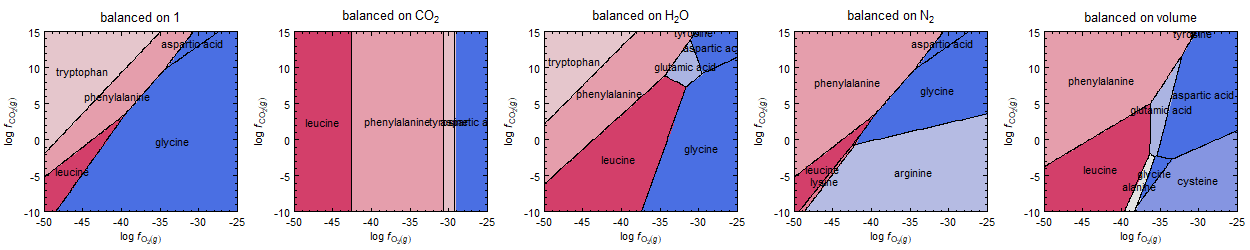
\includegraphics[width=1\linewidth]{anintro_chnosz_files/figure-latex/aafun-1} \caption[Plots of maximum affinity at 250 °C and 265 bar using different reaction balances for 20 amino acids]{Plots of maximum affinity at 250 °C and 265 bar using different reaction balances for 20 amino acids.}\label{fig:aafun}
\end{figure*}

There are some broad similarities---increasing logfO2 favors more
oxidized amino acids---but also substantial differences. It is
interesting that there is more ``going on'' in the middle part of the
diagram showing volume conservation.

\emph{Caveat lector}. These plots demonstrate some possibilities in
CHNOSZ and are not necessarily realistic portrayals of this system. It
does seem odd to balance on a fugacious component like O2 or H2O. Unlike
different choices of basis species, which are thermodynamically
equivalent (\protect\hyperlink{mosaicfun}{see above}), the choice of
balance reflects extra-thermodynamic factors. For instance, the
widespread rule of thumb for balancing mineral reactions on a chemical
component is unrealistic for processes where volume is conserved
\citep{MD98}. While choosing an inappropriate balance leads to
infeasible models, consideration of the different possibilities might
give insight into the conditions affecting the dynamics of some systems.

\section{Activity coefficients}\label{activity-coefficients}

For calculating activity coefficients of charged species,
{\texttt{nonideal()}} uses the extended Debye--Hückel equation as
parameterized by \citet{HKF81} for NaCl-dominated solutions to high
pressure and temperature, or optionally using parameters described in
Chapter 3 of \citet{Alb03}, which are applicable to relatively
low-temperature biochemical reactions. The activity coefficients are
calculated as a function of ionic strength (\emph{I}), temperature, and
charge of each species, without any other species-specific parameters.
Using the default \texttt{Helgeson} method, the extended term parameter
(``B-dot'') is derived from data of \citet{Hel69} and Helgeson et al.
(1981), and extrapolations of \citet{MSS13}.

\subsection{Transformation of
variables}\label{transformation-of-variables}

Following the main workflow of CHNOSZ, {\texttt{nonideal()}} normally
does not need to be used directly. Intead, invoke the calculations by
setting the \texttt{IS} argument in {\texttt{subcrt()}} or
{\texttt{affinity()}}. There are a few things to remember when using
activity coefficients:

\begin{itemize}
\item
  H+ is assumed to behave ideally, so its activity coefficient is 1 for
  any ionic strength. You can calculate activity coefficients of H+ by
  setting \texttt{thermo\$opt\$ideal.H\ \textless{}\textless{}-\ FALSE}.
\item
  Using {\texttt{subcrt()}} with \texttt{IS} not equal to zero,
  calculated values of \texttt{G} are the \textbf{adjusted} Gibbs energy
  at specified ionic strength \citep[denoted by
  Δ\emph{G}°(\emph{I});][]{Alb96}.
\item
  Using {\texttt{subcrt()}} with \texttt{IS} not equal to zero, values
  in the \texttt{logact} argument stand for \textbf{log molality} of
  aqueous species in affinity calculations.
\item
  Using {\texttt{affinity()}} with \texttt{IS} not equal to zero, the
  following values stand for \textbf{log molality} of aqueous species:

  \begin{itemize}
  \tightlist
  \item
    values of \texttt{logact} set by {\texttt{basis()}};
  \item
    values of \texttt{logact} set by {\texttt{species()}}.
  \end{itemize}
\item
  Using {\texttt{equilibrate()}} on the output of affinity calculated
  with \texttt{IS} not equal to zero, the following values stand for
  \textbf{log molality} of aqueous species:

  \begin{itemize}
  \tightlist
  \item
    the value of \texttt{loga.balance} used by {\texttt{equilibrate()}}
    (i.e., logarithm of total molality of the balancing basis species);
  \item
    values of \texttt{loga.equil} returned by {\texttt{equilibrate()}}.
  \end{itemize}
\end{itemize}

In other words, the activation of activity coefficients effects a
transformation from activity to molality in the main workflow. A simple
but comprehensive series of calculations demonstrating these
tranformations is in \texttt{tests/testthat/test-logmolality.R}.

Because it is not possible to dynamically change the names of arguments
in the functions, the user should be aware of the transformations
mentioned above. However, the labels on diagrams \emph{can} be
automatically adjusted; accordingly, activities of aqueous species are
relabeled as molalities by {\texttt{diagram()}} when \texttt{IS} is used
in the calculation of {\texttt{affinity()}}.

\subsection{Biochemical example}\label{biochemical-example}

For the following calculations, we change the nonideality method to
\texttt{Alberty}; this is a simpler formulation with parameters that are
suitable for biochemical species at relatively low temperatures:

\begin{Shaded}
\begin{Highlighting}[]
\NormalTok{oldnon <-}\StringTok{ }\KeywordTok{nonideal}\NormalTok{(}\StringTok{"Alberty"}\NormalTok{)}
\end{Highlighting}
\end{Shaded}

Let's take a look at calculated activity coefficients at two
temperatures and their effect on the standard Gibbs energies of
formation (Î''\emph{G}°\emph{f}) of species with different charge:

\begin{Shaded}
\begin{Highlighting}[]
\KeywordTok{subcrt}\NormalTok{(}\KeywordTok{c}\NormalTok{(}\StringTok{"MgATP-2"}\NormalTok{, }\StringTok{"MgHATP-"}\NormalTok{, }\StringTok{"MgH2ATP"}\NormalTok{),}
       \DataTypeTok{T =} \KeywordTok{c}\NormalTok{(}\DecValTok{25}\NormalTok{, }\DecValTok{100}\NormalTok{), }\DataTypeTok{IS =} \KeywordTok{c}\NormalTok{(}\DecValTok{0}\NormalTok{, }\FloatTok{0.25}\NormalTok{), }\DataTypeTok{property =} \StringTok{"G"}\NormalTok{)}\OperatorTok{$}\NormalTok{out}
\end{Highlighting}
\end{Shaded}

\begin{verbatim}
## $`MgATP-2`
##     T       P       G    loggam   IS
## 1  25 1.00000 -773609  0.000000 0.00
## 2 100 1.01322 -780416 -0.656185 0.25
## 
## $`MgHATP-`
##     T       P       G    loggam   IS
## 1  25 1.00000 -780994  0.000000 0.00
## 2 100 1.01322 -789617 -0.164046 0.25
## 
## $MgH2ATP
##     T       P       G
## 1  25 1.00000 -786200
## 2 100 1.01322 -795012
\end{verbatim}

The logarithms of the activity coefficients (\texttt{loggam}) are more
negative for the higher-charged species, as well as at higher
temperature, and have a stabilizing effect. That is, the adjusted Gibbs
energies at \emph{I} \textgreater{} 0 are less than the standard Gibbs
energies at \emph{I} = 0.

We can use these calculations to make some speciation plots, similar to
Figures 1.2--1.5 in Alberty (2003). These figures show the distribution
of differently charged species of adenosine triphosphate (ATP) as a
function of pH, and the average number of H+ and Mg+2 bound to ATP in
solution as a function of pH or pMg (-log\emph{a}Mg+2).

Use {\texttt{info()}} to see what ATP species are available. The sources
of high-temperature thermodynamic data for these species are two papers
by LaRowe and Helgeson \citetext{\citeyear{LH06a}; \citeyear{LH06b}}.

\begin{Shaded}
\begin{Highlighting}[]
\KeywordTok{info}\NormalTok{(}\StringTok{" ATP"}\NormalTok{)}
\end{Highlighting}
\end{Shaded}

The plots for this system in Alberty's book were made for \emph{I} =
0.25 M and \emph{T} = 25 °C. As a demonstration of CHNOSZ's
capabilities, we can assign a temperature of 100 °C.

\begin{Shaded}
\begin{Highlighting}[]
\NormalTok{T <-}\StringTok{ }\DecValTok{100}
\end{Highlighting}
\end{Shaded}

Use the following commands to set the basis species, add the variously
protonated ATP species, calculate the affinities of the formation
reactions, equilibrate the system, and make a degree of formation (α)
or mole fraction diagram. This is similar to Figure 1.3 of Alberty
(2003), but is calculated for \emph{I} = 0 M and \emph{T} = 100 °C:

\begin{marginfigure}
To make the code more readable, commands for plotting titles and legends
are not shown. All of the commands are available in the source of this
document.
\end{marginfigure}

\begin{Shaded}
\begin{Highlighting}[]
\KeywordTok{basis}\NormalTok{(}\StringTok{"MgCHNOPS+"}\NormalTok{)}
\KeywordTok{species}\NormalTok{(}\KeywordTok{c}\NormalTok{(}\StringTok{"ATP-4"}\NormalTok{, }\StringTok{"HATP-3"}\NormalTok{, }\StringTok{"H2ATP-2"}\NormalTok{, }\StringTok{"H3ATP-"}\NormalTok{, }\StringTok{"H4ATP"}\NormalTok{))}
\NormalTok{a <-}\StringTok{ }\KeywordTok{affinity}\NormalTok{(}\DataTypeTok{pH =} \KeywordTok{c}\NormalTok{(}\DecValTok{3}\NormalTok{, }\DecValTok{9}\NormalTok{), }\DataTypeTok{T =}\NormalTok{ T)}
\NormalTok{e <-}\StringTok{ }\KeywordTok{equilibrate}\NormalTok{(a)}
\NormalTok{d <-}\StringTok{ }\KeywordTok{diagram}\NormalTok{(e, }\DataTypeTok{alpha =} \OtherTok{TRUE}\NormalTok{, }\DataTypeTok{tplot =} \OtherTok{FALSE}\NormalTok{)}
\end{Highlighting}
\end{Shaded}

Note that we have saved the numeric results of {\texttt{diagram()}},
i.e.~the degrees of formation of the species (α). With that, we can
calculate and plot the average number of protons bound per ATP molecule.
To do so, we use R's \texttt{rbind()} and \texttt{do.call()} to turn
\texttt{alpha} into a matrix, then multiply by the number of protons
bound to each species, and sum the columns to get the total
(i.e.~average proton number, \emph{N}H+):

\begin{Shaded}
\begin{Highlighting}[]
\NormalTok{alphas <-}\StringTok{ }\KeywordTok{do.call}\NormalTok{(rbind, d}\OperatorTok{$}\NormalTok{plotvals)}
\NormalTok{nH <-}\StringTok{ }\NormalTok{alphas }\OperatorTok{*}\StringTok{ }\DecValTok{0}\OperatorTok{:}\DecValTok{4}
\NormalTok{Hlab <-}\StringTok{ }\KeywordTok{substitute}\NormalTok{(}\KeywordTok{italic}\NormalTok{(N)[H}\OperatorTok{^}\StringTok{`}\DataTypeTok{+}\StringTok{`}\NormalTok{])}
\KeywordTok{plot}\NormalTok{(a}\OperatorTok{$}\NormalTok{vals[[}\DecValTok{1}\NormalTok{]], }\KeywordTok{colSums}\NormalTok{(nH), }\DataTypeTok{type =} \StringTok{"l"}\NormalTok{, }\DataTypeTok{xlab =} \StringTok{"pH"}\NormalTok{, }\DataTypeTok{ylab=}\NormalTok{Hlab, }\DataTypeTok{lty=}\DecValTok{2}\NormalTok{, }\DataTypeTok{col=}\DecValTok{2}\NormalTok{)}
\end{Highlighting}
\end{Shaded}

Adding the \texttt{IS} argument to {\texttt{affinity()}}, we can now
plot \emph{N}H+ at the given ionic strength. Here we set
\texttt{plot.it\ =\ FALSE} in \texttt{diagram()} because we use the
computed α to make our own plot. This is similar to Figure 1.3 of
Alberty (2003), but at higher temperature:

\begin{Shaded}
\begin{Highlighting}[]
\NormalTok{a <-}\StringTok{ }\KeywordTok{affinity}\NormalTok{(}\DataTypeTok{pH =} \KeywordTok{c}\NormalTok{(}\DecValTok{3}\NormalTok{, }\DecValTok{9}\NormalTok{), }\DataTypeTok{IS =} \FloatTok{0.25}\NormalTok{, }\DataTypeTok{T =}\NormalTok{ T)}
\NormalTok{e <-}\StringTok{ }\KeywordTok{equilibrate}\NormalTok{(a)}
\NormalTok{d <-}\StringTok{ }\KeywordTok{diagram}\NormalTok{(e, }\DataTypeTok{alpha =} \OtherTok{TRUE}\NormalTok{, }\DataTypeTok{plot.it =} \OtherTok{FALSE}\NormalTok{)}
\NormalTok{alphas <-}\StringTok{ }\KeywordTok{do.call}\NormalTok{(rbind, d}\OperatorTok{$}\NormalTok{plotvals)}
\NormalTok{nH <-}\StringTok{ }\NormalTok{alphas }\OperatorTok{*}\StringTok{ }\DecValTok{0}\OperatorTok{:}\DecValTok{4}
\KeywordTok{lines}\NormalTok{(a}\OperatorTok{$}\NormalTok{vals[[}\DecValTok{1}\NormalTok{]], }\KeywordTok{colSums}\NormalTok{(nH))}
\end{Highlighting}
\end{Shaded}

Next, we add the Mg+2-complexed ATP species:

\begin{Shaded}
\begin{Highlighting}[]
\KeywordTok{species}\NormalTok{(}\KeywordTok{c}\NormalTok{(}\StringTok{"MgATP-2"}\NormalTok{, }\StringTok{"MgHATP-"}\NormalTok{, }\StringTok{"MgH2ATP"}\NormalTok{, }\StringTok{"Mg2ATP"}\NormalTok{))}
\end{Highlighting}
\end{Shaded}

Here is a function to calculate and plot \emph{N}H+ for a given pMg:

\begin{Shaded}
\begin{Highlighting}[]
\NormalTok{Hplot <-}\StringTok{ }\ControlFlowTok{function}\NormalTok{(pMg, }\DataTypeTok{IS =} \FloatTok{0.25}\NormalTok{) \{}
  \KeywordTok{basis}\NormalTok{(}\StringTok{"Mg+2"}\NormalTok{, }\OperatorTok{-}\NormalTok{pMg)}
\NormalTok{  a <-}\StringTok{ }\KeywordTok{affinity}\NormalTok{(}\DataTypeTok{pH =} \KeywordTok{c}\NormalTok{(}\DecValTok{3}\NormalTok{, }\DecValTok{9}\NormalTok{), }\DataTypeTok{IS =}\NormalTok{ IS, }\DataTypeTok{T =}\NormalTok{ T)}
\NormalTok{  e <-}\StringTok{ }\KeywordTok{equilibrate}\NormalTok{(a)}
\NormalTok{  d <-}\StringTok{ }\KeywordTok{diagram}\NormalTok{(e, }\DataTypeTok{alpha =} \OtherTok{TRUE}\NormalTok{, }\DataTypeTok{plot.it =} \OtherTok{FALSE}\NormalTok{)}
\NormalTok{  alphas <-}\StringTok{ }\KeywordTok{do.call}\NormalTok{(rbind, d}\OperatorTok{$}\NormalTok{plotvals)}
\NormalTok{  NH <-}\StringTok{ }\NormalTok{alphas }\OperatorTok{*}\StringTok{ }\KeywordTok{c}\NormalTok{(}\DecValTok{0}\OperatorTok{:}\DecValTok{4}\NormalTok{, }\DecValTok{0}\NormalTok{, }\DecValTok{1}\NormalTok{, }\DecValTok{2}\NormalTok{, }\DecValTok{0}\NormalTok{)}
  \KeywordTok{lines}\NormalTok{(a}\OperatorTok{$}\NormalTok{vals[[}\DecValTok{1}\NormalTok{]], }\KeywordTok{colSums}\NormalTok{(NH), }\DataTypeTok{lty =} \DecValTok{7} \OperatorTok{-}\StringTok{ }\NormalTok{pMg, }\DataTypeTok{col =} \DecValTok{7} \OperatorTok{-}\StringTok{ }\NormalTok{pMg)}
\NormalTok{\}}
\end{Highlighting}
\end{Shaded}

With that function in hand, we plot the lines corresponding to pMg = 2
to 6. This is similar to Figure 1.4 of Alberty (2003):

\begin{Shaded}
\begin{Highlighting}[]
\KeywordTok{plot}\NormalTok{(}\KeywordTok{c}\NormalTok{(}\DecValTok{3}\NormalTok{, }\DecValTok{9}\NormalTok{), }\KeywordTok{c}\NormalTok{(}\DecValTok{0}\NormalTok{, }\DecValTok{2}\NormalTok{), }\DataTypeTok{type =} \StringTok{"n"}\NormalTok{, }\DataTypeTok{xlab =} \StringTok{"pH"}\NormalTok{, }\DataTypeTok{ylab =}\NormalTok{ Hlab)}
\KeywordTok{lapply}\NormalTok{(}\DecValTok{2}\OperatorTok{:}\DecValTok{6}\NormalTok{, Hplot)}
\end{Highlighting}
\end{Shaded}

The next function calculates and plots the average number of Mg+2 bound
to ATP (\emph{N}Mg+2) for a given pH. Here we multiply \texttt{alpha} by
the number of Mg+2 in each species, and negate log\emph{a}Mg+2 (the
variable used in {\texttt{affinity()}}) to get pMg:

\begin{Shaded}
\begin{Highlighting}[]
\NormalTok{Mgplot <-}\StringTok{ }\ControlFlowTok{function}\NormalTok{(pH, }\DataTypeTok{IS =} \FloatTok{0.25}\NormalTok{) \{}
  \KeywordTok{basis}\NormalTok{(}\StringTok{"pH"}\NormalTok{, pH)}
\NormalTok{  a <-}\StringTok{ }\KeywordTok{affinity}\NormalTok{(}\StringTok{`}\DataTypeTok{Mg+2}\StringTok{`}\NormalTok{ =}\StringTok{ }\KeywordTok{c}\NormalTok{(}\OperatorTok{-}\DecValTok{2}\NormalTok{, }\OperatorTok{-}\DecValTok{7}\NormalTok{), }\DataTypeTok{IS =}\NormalTok{ IS, }\DataTypeTok{T =}\NormalTok{ T)}
\NormalTok{  e <-}\StringTok{ }\KeywordTok{equilibrate}\NormalTok{(a)}
\NormalTok{  d <-}\StringTok{ }\KeywordTok{diagram}\NormalTok{(e, }\DataTypeTok{alpha =} \OtherTok{TRUE}\NormalTok{, }\DataTypeTok{plot.it =} \OtherTok{FALSE}\NormalTok{)}
\NormalTok{  alphas <-}\StringTok{ }\KeywordTok{do.call}\NormalTok{(rbind, d}\OperatorTok{$}\NormalTok{plotvals)}
\NormalTok{  NMg <-}\StringTok{ }\NormalTok{alphas }\OperatorTok{*}\StringTok{ }\KeywordTok{species}\NormalTok{()}\OperatorTok{$}\StringTok{`}\DataTypeTok{Mg+}\StringTok{`}
  \KeywordTok{lines}\NormalTok{(}\OperatorTok{-}\NormalTok{a}\OperatorTok{$}\NormalTok{vals[[}\DecValTok{1}\NormalTok{]], }\KeywordTok{colSums}\NormalTok{(NMg), }\DataTypeTok{lty =} \DecValTok{10} \OperatorTok{-}\StringTok{ }\NormalTok{pH, }\DataTypeTok{col =} \DecValTok{10} \OperatorTok{-}\StringTok{ }\NormalTok{pH)}
\NormalTok{\}}
\end{Highlighting}
\end{Shaded}

Using that function, we plot the lines corresponding to pH = 3 to 9.
This is similar to Figure 1.5 of Alberty (2003):

\begin{Shaded}
\begin{Highlighting}[]
\NormalTok{Mglab <-}\StringTok{ }\KeywordTok{substitute}\NormalTok{(}\KeywordTok{italic}\NormalTok{(N)[Mg}\OperatorTok{^}\StringTok{`}\DataTypeTok{+2}\StringTok{`}\NormalTok{])}
\KeywordTok{plot}\NormalTok{(}\KeywordTok{c}\NormalTok{(}\DecValTok{2}\NormalTok{, }\DecValTok{7}\NormalTok{), }\KeywordTok{c}\NormalTok{(}\DecValTok{0}\NormalTok{, }\FloatTok{1.2}\NormalTok{), }\DataTypeTok{type =} \StringTok{"n"}\NormalTok{, }\DataTypeTok{xlab =} \StringTok{"pMg"}\NormalTok{, }\DataTypeTok{ylab =}\NormalTok{ Mglab)}
\KeywordTok{lapply}\NormalTok{(}\DecValTok{3}\OperatorTok{:}\DecValTok{9}\NormalTok{, Mgplot)}
\end{Highlighting}
\end{Shaded}

\begin{figure*}
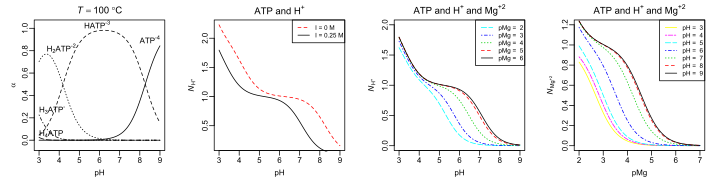
\includegraphics[width=1\linewidth]{anintro_chnosz_files/figure-latex/ATP-1} \caption[Binding of H<sup>+</sup> and Mg<sup>+2</sup> to ATP at 100 °C and *I* = 0 M (first plot) or *I* = 0.25 M (third and fourth plots)]{Binding of H<sup>+</sup> and Mg<sup>+2</sup> to ATP at 100 °C and *I* = 0 M (first plot) or *I* = 0.25 M (third and fourth plots).}\label{fig:ATP}
\end{figure*}

We have calculated the distribution of ATP species and average binding
number of H+ and Mg+2 for given pH, pMg, ionic strength, and
temperature. Accounting for the distribution of chemical species lends
itself to thermodynamic models for reactions between reactants that have
multiple ionized and complexed states. In contrast, Alberty (2003) and
others propose models for biochemical reactions where the ionized and
complexed species are combined into a single representation. Those
models invoke Legendre-transformed thermodynamic properties, such as
transformed Gibbs energies that are tabulated for specified pH, pMg, and
ionic strength. Although the conceptual pathways are different, the two
approaches lead to equivalent results concerning the energetics of the
overall reactions and the conditions for equilibrium \citep{SVI12}. The
example here shows how the required calculations can be performed at the
species level using conventional standard Gibbs energies for species
referenced to infinite dilution (zero ionic strength). The effects of
ionic strength are modeled ``on the fly'' in CHNOSZ by setting the
\texttt{IS} argument in {\texttt{subcrt()}} or {\texttt{affinity()}} to
invoke the nonideality model on top of the standard Gibbs energies of
species.

Now that we're finished, we can reset the nonideality method to the
default. (This really isn't needed here, because there aren't any
nonideality calculations below):

\begin{Shaded}
\begin{Highlighting}[]
\KeywordTok{nonideal}\NormalTok{(oldnon)}
\end{Highlighting}
\end{Shaded}

\section{Proteins}\label{proteins}

Proteins in CHNOSZ are handled a little bit differently from other
species. Amino acid group additivity is used to obtain the thermodynamic
properties of proteins. Therefore, CHNOSZ has a data file with amino
acid compositions of selected proteins, as well as functions for reading
and downloading amino acid sequence data.

When proteins in CHNOSZ are identified by name, they include an
underscore, such as in \texttt{LYSC\_CHICK} (chicken lysozyme C). Use
{\texttt{pinfo()}} to search for one or more proteins by name; multiple
proteins from the same organism can be specified using the
\texttt{organism} argument. The name search returns the rownumbers of
\texttt{thermo\$protein} (i.e. \texttt{iprotein}, the protein indices).
Supply those protein indices to {\texttt{pinfo()}} to get the amino acid
compositions:

\begin{Shaded}
\begin{Highlighting}[]
\NormalTok{p1 <-}\StringTok{ }\KeywordTok{pinfo}\NormalTok{(}\StringTok{"LYSC_CHICK"}\NormalTok{)}
\NormalTok{p2 <-}\StringTok{ }\KeywordTok{pinfo}\NormalTok{(}\KeywordTok{c}\NormalTok{(}\StringTok{"SHH"}\NormalTok{, }\StringTok{"OLIG2"}\NormalTok{), }\StringTok{"HUMAN"}\NormalTok{)}
\KeywordTok{pinfo}\NormalTok{(}\KeywordTok{c}\NormalTok{(p1, p2))}
\end{Highlighting}
\end{Shaded}

\begin{verbatim}
##     protein organism     ref    abbrv chains Ala Cys Asp Glu Phe Gly His Ile
## 6      LYSC    CHICK UniProt   P00698      1  12   8   7   2   3  12   1   6
## 452     SHH    HUMAN UniProt Q15465.N      1  14   3  10  14   5  16   6   7
## 453   OLIG2    HUMAN UniProt   Q13516      1  51   5  10  10   5  35  18   7
##     Lys Leu Met Asn Pro Gln Arg Ser Thr Val Trp Tyr
## 6     6   8   2  14   2   3  11  10   7   6   6   3
## 452  15  11   3   8   7   3  13  12   8   9   3   7
## 453  14  29  11   4  31   5  13  50  11  10   1   3
\end{verbatim}

The length and chemical formula of one or more proteins are returned by
{\texttt{protein.length()}} and {\texttt{protein.formula()}}. We can
calculate the formula of the protein, and the per-residue formula, and
show that both have the same average oxidation state of carbon:

\begin{marginfigure}
These functions accept either names or the protein indices
(\texttt{iprotein}).
\end{marginfigure}

\begin{Shaded}
\begin{Highlighting}[]
\NormalTok{pl <-}\StringTok{ }\KeywordTok{protein.length}\NormalTok{(}\StringTok{"LYSC_CHICK"}\NormalTok{)}
\NormalTok{pf <-}\StringTok{ }\KeywordTok{protein.formula}\NormalTok{(}\StringTok{"LYSC_CHICK"}\NormalTok{)}
\KeywordTok{list}\NormalTok{(}\DataTypeTok{length =}\NormalTok{ pl, }\DataTypeTok{protein =}\NormalTok{ pf, }\DataTypeTok{residue =}\NormalTok{ pf }\OperatorTok{/}\StringTok{ }\NormalTok{pl,}
     \DataTypeTok{ZC_protein =} \KeywordTok{ZC}\NormalTok{(pf), }\DataTypeTok{ZC_residue =} \KeywordTok{ZC}\NormalTok{(pf }\OperatorTok{/}\StringTok{ }\NormalTok{pl))}
\end{Highlighting}
\end{Shaded}

\begin{verbatim}
## $length
## [1] 129
## 
## $protein
##              C   H   N   O  S
## LYSC_CHICK 613 959 193 185 10
## 
## $residue
##                  C       H       N       O         S
## LYSC_CHICK 4.75194 7.43411 1.49612 1.43411 0.0775194
## 
## $ZC_protein
## [1] 0.0163132
## 
## $ZC_residue
## [1] 0.0163132
\end{verbatim}

\subsection{Group additivity and
ionization}\label{group-additivity-and-ionization}

The group additivity calculations for proteins are based on equations
and data from \citet{AH00}, \citet{DLH06}, and \citet{LD12}. There are
two major options for the calculations: whether to calculate properties
for crystalline or aqueous groups, and, for the latter, whether to model
the ionization of the sidechain and terminal groups as a function of pH
(and \emph{T} and \emph{P}). By default, additivity of aqueous groups is
used, but the ionization calculations are not available in
\texttt{subcrt()}:

\begin{Shaded}
\begin{Highlighting}[]
\KeywordTok{subcrt}\NormalTok{(}\StringTok{"LYSC_CHICK"}\NormalTok{)}\OperatorTok{$}\NormalTok{out[[}\DecValTok{1}\NormalTok{]][}\DecValTok{1}\OperatorTok{:}\DecValTok{6}\NormalTok{, ]}
\end{Highlighting}
\end{Shaded}

\begin{verbatim}
##        T       P      rho    logK        G         H       S       V      Cp
## 1   0.01 1.00000 0.999829 3217.68 -4021765 -10423733 3685.29 10049.2 4409.32
## 2  25.00 1.00000 0.997061 3019.80 -4119738 -10283083 4176.74 10421.0 6415.52
## 3  50.00 1.00000 0.988030 2861.40 -4230972 -10113250 4723.39 10600.2 7073.98
## 4  75.00 1.00000 0.974864 2734.31 -4355838  -9932209 5262.87 10708.1 7376.58
## 5 100.00 1.01322 0.958393 2632.00 -4493930  -9745475 5780.77 10782.9 7548.44
## 6 125.00 2.32014 0.939073 2549.29 -4644330  -9554920 6274.14 10840.9 7665.20
\end{verbatim}

Let's compare experimental values of heat capacity of four proteins,
from \citet{PM90}, with those calculated using group additivity. After
dividing Privalov and Makhatadze's experimental values by the lengths of
the proteins to get per-residue values, we convert those to calories,
then plot them.

\begin{marginfigure}
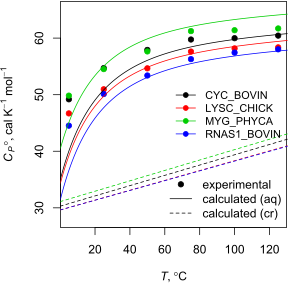
\includegraphics[width=1\linewidth]{anintro_chnosz_files/figure-latex/protein_Cp-1} \caption[The heat capacity calculated by group additivity closely approximates experimental values for aqueous proteins]{The heat capacity calculated by group additivity closely approximates experimental values for aqueous proteins. For a related figure showing the effects of ionization in the calculations, see <span style="color:blue">?ionize.aa</span>.}\label{fig:protein_Cp}
\end{marginfigure}

\begin{Shaded}
\begin{Highlighting}[]
\NormalTok{PM90 <-}\StringTok{ }\KeywordTok{read.csv}\NormalTok{(}\KeywordTok{system.file}\NormalTok{(}\StringTok{"extdata/cpetc/PM90.csv"}\NormalTok{, }\DataTypeTok{package =} \StringTok{"CHNOSZ"}\NormalTok{))}
\NormalTok{plength <-}\StringTok{ }\KeywordTok{protein.length}\NormalTok{(}\KeywordTok{colnames}\NormalTok{(PM90)[}\DecValTok{2}\OperatorTok{:}\DecValTok{5}\NormalTok{])}
\NormalTok{Cp_expt <-}\StringTok{ }\KeywordTok{t}\NormalTok{(}\KeywordTok{t}\NormalTok{(PM90[, }\DecValTok{2}\OperatorTok{:}\DecValTok{5}\NormalTok{]) }\OperatorTok{/}\StringTok{ }\NormalTok{plength)}
\KeywordTok{matplot}\NormalTok{(PM90[, }\DecValTok{1}\NormalTok{], }\KeywordTok{convert}\NormalTok{(Cp_expt, }\StringTok{"cal"}\NormalTok{), }\DataTypeTok{type =} \StringTok{"p"}\NormalTok{, }\DataTypeTok{pch =} \DecValTok{19}\NormalTok{,}
        \DataTypeTok{xlab =} \KeywordTok{axis.label}\NormalTok{(}\StringTok{"T"}\NormalTok{), }\DataTypeTok{ylab =} \KeywordTok{axis.label}\NormalTok{(}\StringTok{"Cp0"}\NormalTok{), }\DataTypeTok{ylim =} \KeywordTok{c}\NormalTok{(}\DecValTok{28}\NormalTok{, }\DecValTok{65}\NormalTok{))}
\end{Highlighting}
\end{Shaded}

The loop calculates the properties of each protein using group
additivity with aqueous or crystalline groups, then plots the
per-residue values.

\begin{Shaded}
\begin{Highlighting}[]
\ControlFlowTok{for}\NormalTok{(i }\ControlFlowTok{in} \DecValTok{1}\OperatorTok{:}\DecValTok{4}\NormalTok{) \{}
\NormalTok{  pname <-}\StringTok{ }\KeywordTok{colnames}\NormalTok{(Cp_expt)[i]}
\NormalTok{  aq <-}\StringTok{ }\KeywordTok{subcrt}\NormalTok{(pname, }\StringTok{"aq"}\NormalTok{, }\DataTypeTok{T =} \KeywordTok{seq}\NormalTok{(}\DecValTok{0}\NormalTok{, }\DecValTok{150}\NormalTok{))}\OperatorTok{$}\NormalTok{out[[}\DecValTok{1}\NormalTok{]]}
\NormalTok{  cr <-}\StringTok{ }\KeywordTok{subcrt}\NormalTok{(pname, }\StringTok{"cr"}\NormalTok{, }\DataTypeTok{T =} \KeywordTok{seq}\NormalTok{(}\DecValTok{0}\NormalTok{, }\DecValTok{150}\NormalTok{))}\OperatorTok{$}\NormalTok{out[[}\DecValTok{1}\NormalTok{]]}
  \KeywordTok{lines}\NormalTok{(aq}\OperatorTok{$}\NormalTok{T, aq}\OperatorTok{$}\NormalTok{Cp }\OperatorTok{/}\StringTok{ }\NormalTok{plength[i], }\DataTypeTok{col =}\NormalTok{ i)}
  \KeywordTok{lines}\NormalTok{(cr}\OperatorTok{$}\NormalTok{T, cr}\OperatorTok{$}\NormalTok{Cp }\OperatorTok{/}\StringTok{ }\NormalTok{plength[i], }\DataTypeTok{col =}\NormalTok{ i, }\DataTypeTok{lty =} \DecValTok{2}\NormalTok{)}
\NormalTok{\}}
\KeywordTok{legend}\NormalTok{(}\StringTok{"right"}\NormalTok{, }\DataTypeTok{legend =} \KeywordTok{colnames}\NormalTok{(Cp_expt),}
       \DataTypeTok{col =} \DecValTok{1}\OperatorTok{:}\DecValTok{4}\NormalTok{, }\DataTypeTok{pch =} \DecValTok{19}\NormalTok{, }\DataTypeTok{lty =} \DecValTok{1}\NormalTok{, }\DataTypeTok{bty =} \StringTok{"n"}\NormalTok{, }\DataTypeTok{cex =} \FloatTok{0.9}\NormalTok{)}
\KeywordTok{legend}\NormalTok{(}\StringTok{"bottomright"}\NormalTok{, }\DataTypeTok{legend =} \KeywordTok{c}\NormalTok{(}\StringTok{"experimental"}\NormalTok{, }\StringTok{"calculated (aq)"}\NormalTok{,}
       \StringTok{"calculated (cr)"}\NormalTok{), }\DataTypeTok{lty =} \KeywordTok{c}\NormalTok{(}\OtherTok{NA}\NormalTok{, }\DecValTok{1}\NormalTok{, }\DecValTok{2}\NormalTok{), }\DataTypeTok{pch =} \KeywordTok{c}\NormalTok{(}\DecValTok{19}\NormalTok{, }\OtherTok{NA}\NormalTok{, }\OtherTok{NA}\NormalTok{), }\DataTypeTok{bty =} \StringTok{"n"}\NormalTok{)}
\end{Highlighting}
\end{Shaded}

Although {\texttt{subcrt()}} has no provision for protein ionization,
the properties of ionization can be calculated via
{\texttt{affinity()}}, which calls {\texttt{ionize.aa()}} if a charged
species is in the basis.

\begin{marginfigure}
Whether to calculate properties using aqueous or crystalline groups is
determined by the value of
\texttt{thermo\textbackslash{}\$opt\textbackslash{}\$state}; if it is
changed from its default of \texttt{aq} to \texttt{cr}, no ionization is
possible.
\end{marginfigure}

The following plot shows the calculated affinity of reaction between
nonionized proteins and their ionized forms as a function of pH. Charged
and uncharged sets of basis species are used to to activate and suppress
the ionization calculations. The calculation of affinity for the ionized
proteins returns multiple values (as a function of pH), but there is
only one value of affinity returned for the nonionized proteins, so we
need to use R's \texttt{as.numeric()} to avoid subtracting
nonconformable arrays:

\begin{marginfigure}
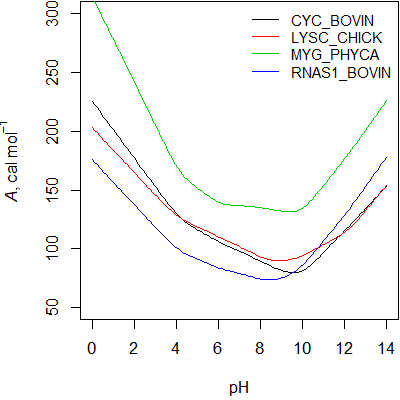
\includegraphics[width=1\linewidth]{anintro_chnosz_files/figure-latex/protein_ionization-1} \caption[Affinity of ionization of proteins]{Affinity of ionization of proteins. See [<span style="color:blue">demo(ionize)</span>](../demo) for ionization properties calculated as a function of temperature and pH.}\label{fig:protein_ionization}
\end{marginfigure}

\begin{Shaded}
\begin{Highlighting}[]
\NormalTok{ip <-}\StringTok{ }\KeywordTok{pinfo}\NormalTok{(}\KeywordTok{c}\NormalTok{(}\StringTok{"CYC_BOVIN"}\NormalTok{, }\StringTok{"LYSC_CHICK"}\NormalTok{, }\StringTok{"MYG_PHYCA"}\NormalTok{, }\StringTok{"RNAS1_BOVIN"}\NormalTok{))}
\KeywordTok{basis}\NormalTok{(}\StringTok{"CHNOS+"}\NormalTok{)}
\NormalTok{a_ion <-}\StringTok{ }\KeywordTok{affinity}\NormalTok{(}\DataTypeTok{pH =} \KeywordTok{c}\NormalTok{(}\DecValTok{0}\NormalTok{, }\DecValTok{14}\NormalTok{), }\DataTypeTok{iprotein =}\NormalTok{ ip)}
\KeywordTok{basis}\NormalTok{(}\StringTok{"CHNOS"}\NormalTok{)}
\NormalTok{a_nonion <-}\StringTok{ }\KeywordTok{affinity}\NormalTok{(}\DataTypeTok{iprotein =}\NormalTok{ ip)}
\KeywordTok{plot}\NormalTok{(}\KeywordTok{c}\NormalTok{(}\DecValTok{0}\NormalTok{, }\DecValTok{14}\NormalTok{), }\KeywordTok{c}\NormalTok{(}\DecValTok{50}\NormalTok{, }\DecValTok{300}\NormalTok{), }\DataTypeTok{xlab =} \StringTok{"pH"}\NormalTok{, }\DataTypeTok{ylab =} \KeywordTok{axis.label}\NormalTok{(}\StringTok{"A"}\NormalTok{), }\DataTypeTok{type =} \StringTok{"n"}\NormalTok{)}
\ControlFlowTok{for}\NormalTok{(i }\ControlFlowTok{in} \DecValTok{1}\OperatorTok{:}\DecValTok{4}\NormalTok{) \{}
\NormalTok{  A_ion <-}\StringTok{ }\KeywordTok{as.numeric}\NormalTok{(a_ion}\OperatorTok{$}\NormalTok{values[[i]])}
\NormalTok{  A_nonion <-}\StringTok{ }\KeywordTok{as.numeric}\NormalTok{(a_nonion}\OperatorTok{$}\NormalTok{values[[i]])}
  \KeywordTok{lines}\NormalTok{(a_ion}\OperatorTok{$}\NormalTok{vals[[}\DecValTok{1}\NormalTok{]], A_ion }\OperatorTok{-}\StringTok{ }\NormalTok{A_nonion, }\DataTypeTok{col=}\NormalTok{i)}
\NormalTok{\}}
\KeywordTok{legend}\NormalTok{(}\StringTok{"topright"}\NormalTok{, }\DataTypeTok{legend =}\NormalTok{ a_ion}\OperatorTok{$}\NormalTok{species}\OperatorTok{$}\NormalTok{name,}
       \DataTypeTok{col =} \DecValTok{1}\OperatorTok{:}\DecValTok{4}\NormalTok{, }\DataTypeTok{lty =} \DecValTok{1}\NormalTok{, }\DataTypeTok{bty =} \StringTok{"n"}\NormalTok{, }\DataTypeTok{cex =} \FloatTok{0.9}\NormalTok{)}
\end{Highlighting}
\end{Shaded}

The affinity is always positive, showing the strong energetic drive for
ionization of proteins in aqueous solution. The degrees of ionization of
amino and carboxyl groups increase at low and high pH, respectively,
giving rise to the U-shaped lines.

There, we used the indices returned by {\texttt{pinfo()}} in the
\texttt{iprotein} argument of {\texttt{affinity()}} to specify the
proteins in the calculation. That approach utilizes some optimizations
that can be realized due to group additivity, and is useful for
calculations involving many proteins. An alternative, but slower,
approach is to identify the proteins to {\texttt{species()}}; this
produces results that are equivalent to using the \texttt{iprotein}
argument:

\begin{Shaded}
\begin{Highlighting}[]
\KeywordTok{species}\NormalTok{(}\KeywordTok{c}\NormalTok{(}\StringTok{"CYC_BOVIN"}\NormalTok{, }\StringTok{"LYSC_CHICK"}\NormalTok{, }\StringTok{"MYG_PHYCA"}\NormalTok{, }\StringTok{"RNAS1_BOVIN"}\NormalTok{))}
\NormalTok{a_nonion_species <-}\StringTok{ }\KeywordTok{affinity}\NormalTok{()}
\end{Highlighting}
\end{Shaded}

\begin{Shaded}
\begin{Highlighting}[]
\KeywordTok{unlist}\NormalTok{(a_nonion_species}\OperatorTok{$}\NormalTok{values)}
\end{Highlighting}
\end{Shaded}

\begin{verbatim}
##      3590      3589      3593      3595 
## -122.5026 -700.5444  -50.6508 -731.8601
\end{verbatim}

\begin{marginfigure}
The \texttt{ispecies} index (top) refers to the rownumber of
\texttt{thermo\textbackslash{}\$species}; that is distinct from the
\texttt{iprotein} index (bottom, printed as negative integers), which
refers to the rownumber of \texttt{thermo\textbackslash{}\$protein}.
\end{marginfigure}

\begin{Shaded}
\begin{Highlighting}[]
\KeywordTok{unlist}\NormalTok{(a_nonion}\OperatorTok{$}\NormalTok{values)}
\end{Highlighting}
\end{Shaded}

\begin{verbatim}
##        -5        -6        -7        -9 
## -122.5026 -700.5444  -50.6508 -731.8601
\end{verbatim}

\subsection{Compositional analysis}\label{compositional-analysis}

Functions in CHNOSZ make it easy to get the chemical formulas of
proteins from their amino acid compositions. Calculations based on the
formulas, such as the average oxidation state of carbon (ZC), and the
coefficients of basis species in formation reactions, are also
available.

Let's compare the ZC of Rubisco with optimal growth temperature of
organisms, as shown in Figure 6a of \citet{Dic14}. First we read a CSV
file with the IDs of the proteins and the optimal growth temperatures
(\emph{T}opt); the midpoint of the range of \emph{T}opt is used for
plotting. Then we use {\texttt{read.fasta()}} to read a FASTA file
holding the amino acid sequences of the proteins; the function returns a
data frame with the amino acid counts. To put the proteins in the right
order, the IDs in the CSV file are matched to the names of the proteins
in the FASTA file. Then, we calculate ZC from the formulas of the
proteins. Next, point symbols are assigned according to domain (Archaea,
Bacteria, Eukaryota); numbers inside the symbols show the ordering of
\emph{T}opt in three temperature ranges (0--35 °C, 37.5--60 °C, and
65--100 °C).

\begin{marginfigure}
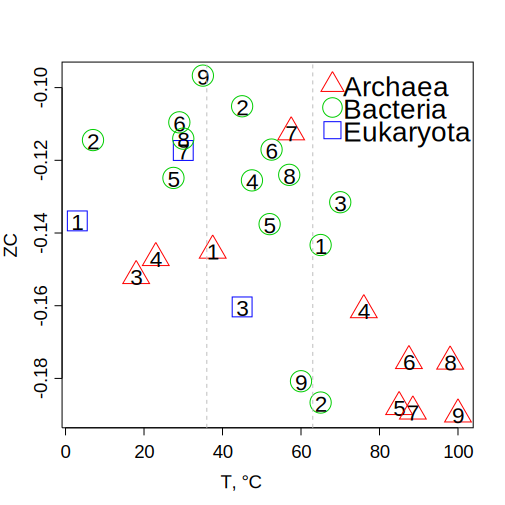
\includegraphics[width=1\linewidth]{anintro_chnosz_files/figure-latex/rubisco_svg-1} \caption[Average oxidation state of carbon in Rubisco compared with optimal growth temperature of organisms]{Average oxidation state of carbon in Rubisco compared with optimal growth temperature of organisms. **This is an interactive image.** Move the mouse over the points to show the names of the organisms, and click to open a reference in a new window. (Made with [**RSVGTipsDevice**](https://cran.r-project.org/package=RSVGTipsDevice) using code that can be found in the source of this document.)}\label{fig:rubisco_svg}
\end{marginfigure}

\begin{Shaded}
\begin{Highlighting}[]
\NormalTok{datfile <-}\StringTok{ }\KeywordTok{system.file}\NormalTok{(}\StringTok{"extdata/cpetc/rubisco.csv"}\NormalTok{, }\DataTypeTok{package =} \StringTok{"CHNOSZ"}\NormalTok{)}
\NormalTok{fastafile <-}\StringTok{ }\KeywordTok{system.file}\NormalTok{(}\StringTok{"extdata/fasta/rubisco.fasta"}\NormalTok{, }\DataTypeTok{package =} \StringTok{"CHNOSZ"}\NormalTok{)}
\NormalTok{dat <-}\StringTok{ }\KeywordTok{read.csv}\NormalTok{(datfile)}
\NormalTok{aa <-}\StringTok{ }\KeywordTok{read.fasta}\NormalTok{(fastafile)}
\NormalTok{Topt <-}\StringTok{ }\NormalTok{(dat}\OperatorTok{$}\NormalTok{T1 }\OperatorTok{+}\StringTok{ }\NormalTok{dat}\OperatorTok{$}\NormalTok{T2) }\OperatorTok{/}\StringTok{ }\DecValTok{2}
\NormalTok{idat <-}\StringTok{ }\KeywordTok{match}\NormalTok{(dat}\OperatorTok{$}\NormalTok{ID, }\KeywordTok{substr}\NormalTok{(aa}\OperatorTok{$}\NormalTok{protein, }\DecValTok{4}\NormalTok{, }\DecValTok{9}\NormalTok{))}
\NormalTok{aa <-}\StringTok{ }\NormalTok{aa[idat, ]}
\NormalTok{ZC <-}\StringTok{ }\KeywordTok{ZC}\NormalTok{(}\KeywordTok{protein.formula}\NormalTok{(aa))}
\NormalTok{pch <-}\StringTok{ }\KeywordTok{match}\NormalTok{(dat}\OperatorTok{$}\NormalTok{domain, }\KeywordTok{c}\NormalTok{(}\StringTok{"E"}\NormalTok{, }\StringTok{"B"}\NormalTok{, }\StringTok{"A"}\NormalTok{)) }\OperatorTok{-}\StringTok{ }\DecValTok{1}
\NormalTok{col <-}\StringTok{ }\KeywordTok{match}\NormalTok{(dat}\OperatorTok{$}\NormalTok{domain, }\KeywordTok{c}\NormalTok{(}\StringTok{"A"}\NormalTok{, }\StringTok{"B"}\NormalTok{, }\StringTok{"E"}\NormalTok{)) }\OperatorTok{+}\StringTok{ }\DecValTok{1}
\KeywordTok{plot}\NormalTok{(Topt, ZC, }\DataTypeTok{pch =}\NormalTok{ pch, }\DataTypeTok{cex =} \DecValTok{2}\NormalTok{, }\DataTypeTok{col =}\NormalTok{ col,}
     \DataTypeTok{xlab =} \KeywordTok{expression}\NormalTok{(}\KeywordTok{list}\NormalTok{(}\KeywordTok{italic}\NormalTok{(T)[opt], degree}\OperatorTok{*}\NormalTok{C)),}
     \DataTypeTok{ylab =} \KeywordTok{expression}\NormalTok{(}\KeywordTok{italic}\NormalTok{(Z)[C]))}
\KeywordTok{text}\NormalTok{(Topt, ZC, }\KeywordTok{rep}\NormalTok{(}\DecValTok{1}\OperatorTok{:}\DecValTok{9}\NormalTok{, }\DecValTok{3}\NormalTok{), }\DataTypeTok{cex =} \FloatTok{0.8}\NormalTok{)}
\KeywordTok{abline}\NormalTok{(}\DataTypeTok{v =} \KeywordTok{c}\NormalTok{(}\DecValTok{36}\NormalTok{, }\DecValTok{63}\NormalTok{), }\DataTypeTok{lty =} \DecValTok{2}\NormalTok{, }\DataTypeTok{col =} \StringTok{"grey"}\NormalTok{)}
\KeywordTok{legend}\NormalTok{(}\StringTok{"topright"}\NormalTok{, }\DataTypeTok{legend =} \KeywordTok{c}\NormalTok{(}\StringTok{"Archaea"}\NormalTok{, }\StringTok{"Bacteria"}\NormalTok{, }\StringTok{"Eukaryota"}\NormalTok{),}
       \DataTypeTok{pch =} \KeywordTok{c}\NormalTok{(}\DecValTok{2}\NormalTok{, }\DecValTok{1}\NormalTok{, }\DecValTok{0}\NormalTok{), }\DataTypeTok{col =} \DecValTok{2}\OperatorTok{:}\DecValTok{4}\NormalTok{, }\DataTypeTok{pt.cex =} \DecValTok{2}\NormalTok{)}
\end{Highlighting}
\end{Shaded}

Let's look at the different ways of representing the chemical
compositions of the proteins. {\texttt{protein.basis()}} returns the
stoichiometry for the formation reaction of each proteins. Dividing by
{\texttt{protein.length()}} gives the per-residue reaction coefficients
(\emph{n}̅). Using the set of basis species we have seen before (CO2,
NH3, H2S, H2O, O2) there is a noticeable correlation between \emph{n}̅O2
and ZC, but even more so between \emph{n}̅H2O and ZC (shown in the plots
on the left).

\begin{marginfigure}
The calculation of \emph{Z}C, which sums elemental ratios, is not
affected by the choice of basis species.
\end{marginfigure}

The \texttt{QEC} keyword to {\texttt{basis()}} loads basis species
including three amino acids (glutamine, glutamic acid, cysteine, H2O,
O2). This basis strengthens the relationship between ZC and \emph{n}̅O2,
but weakens that between ZC and \emph{n}̅H2O (shown in the plots on the
right).

\begin{marginfigure}
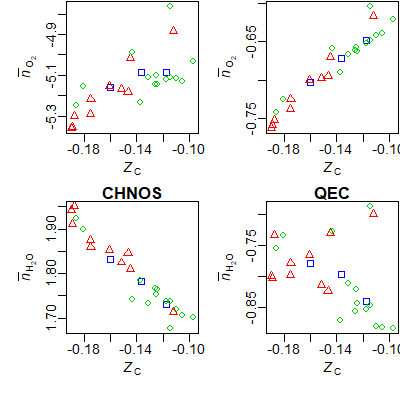
\includegraphics[width=1\linewidth]{anintro_chnosz_files/figure-latex/rubisco_O2-1} \caption[Compositions of proteins projected into different sets of basis species]{Compositions of proteins projected into different sets of basis species.}\label{fig:rubisco_O2}
\end{marginfigure}

\begin{Shaded}
\begin{Highlighting}[]
\KeywordTok{layout}\NormalTok{(}\KeywordTok{matrix}\NormalTok{(}\DecValTok{1}\OperatorTok{:}\DecValTok{4}\NormalTok{, }\DataTypeTok{nrow =} \DecValTok{2}\NormalTok{))}
\KeywordTok{par}\NormalTok{(}\DataTypeTok{mgp =} \KeywordTok{c}\NormalTok{(}\FloatTok{1.8}\NormalTok{, }\FloatTok{0.5}\NormalTok{, }\DecValTok{0}\NormalTok{))}
\NormalTok{pl <-}\StringTok{ }\KeywordTok{protein.length}\NormalTok{(aa)}
\NormalTok{ZClab <-}\StringTok{ }\KeywordTok{axis.label}\NormalTok{(}\StringTok{"ZC"}\NormalTok{)}
\NormalTok{nO2lab <-}\StringTok{ }\KeywordTok{expression}\NormalTok{(}\KeywordTok{bar}\NormalTok{(}\KeywordTok{italic}\NormalTok{(n))[O[}\DecValTok{2}\NormalTok{]])}
\NormalTok{nH2Olab <-}\StringTok{ }\KeywordTok{expression}\NormalTok{(}\KeywordTok{bar}\NormalTok{(}\KeywordTok{italic}\NormalTok{(n))[H[}\DecValTok{2}\NormalTok{]}\OperatorTok{*}\NormalTok{O])}
\KeywordTok{lapply}\NormalTok{(}\KeywordTok{c}\NormalTok{(}\StringTok{"CHNOS"}\NormalTok{, }\StringTok{"QEC"}\NormalTok{), }\ControlFlowTok{function}\NormalTok{(thisbasis) \{}
  \KeywordTok{basis}\NormalTok{(thisbasis)}
\NormalTok{  pb <-}\StringTok{ }\KeywordTok{protein.basis}\NormalTok{(aa)}
\NormalTok{  nO2 <-}\StringTok{ }\NormalTok{pb[, }\StringTok{"O2"}\NormalTok{] }\OperatorTok{/}\StringTok{ }\NormalTok{pl}
  \KeywordTok{plot}\NormalTok{(ZC, nO2, }\DataTypeTok{pch =}\NormalTok{ pch, }\DataTypeTok{col =}\NormalTok{ col, }\DataTypeTok{xlab =}\NormalTok{ ZClab, }\DataTypeTok{ylab =}\NormalTok{ nO2lab)}
\NormalTok{  nH2O <-}\StringTok{ }\NormalTok{pb[, }\StringTok{"H2O"}\NormalTok{] }\OperatorTok{/}\StringTok{ }\NormalTok{pl}
  \KeywordTok{plot}\NormalTok{(ZC, nH2O, }\DataTypeTok{pch =}\NormalTok{ pch, }\DataTypeTok{col =}\NormalTok{ col, }\DataTypeTok{xlab =}\NormalTok{ ZClab, }\DataTypeTok{ylab =}\NormalTok{ nH2Olab)}
  \KeywordTok{mtext}\NormalTok{(thisbasis, }\DataTypeTok{font =} \DecValTok{2}\NormalTok{)}
\NormalTok{\})}
\end{Highlighting}
\end{Shaded}

By projecting the compositions of proteins into the \texttt{QEC} set of
basis species, \emph{n}̅O2 emerges as a strong indicator of oxidation
state, while \emph{n}̅H2O is a relatively uncorrelated (i.e.~independent)
compositional variable. These independent variables make it easier to
distinguish the effects of oxidation and hydration state in proteomic
datasets \citep{Dic17}.

\subsection{Normalization to residues}\label{normalization-to-residues}

As with other systems, a balance must be chosen for calculations of the
metastable equilibrium distribution for proteins. Balancing on the
number of backbone units (the sequence length) seems a reasonable choice
given the polymeric structure of proteins.

\begin{marginfigure}
Balancing on one of the basis species remains a possibility, using the
\texttt{balance} argument in {\texttt{equilibrate()}} or
{\texttt{diagram()}}.
\end{marginfigure}

However, there is an additional consideration: owing to the large size
of proteins compared to the basis species, the distribution of
\emph{proteins} in metastable equilibrium has many orders of magnitude
separation between the activities of the dominant and less-dominant
proteins. The metastable coexistence of the \emph{residues}
(i.e.~per-residue formulas, or residue equivalents) of the same proteins
spans a much smaller range of chemical activities. In CHNOSZ, the
calculation of metastable equilibrium activities of the residue
equivalents is referred to as \emph{normalization}.

\begin{marginfigure}
See the vignette \href{equilibrium.pdf}{{\emph{Equilibrium in CHNOSZ}}}
for other examples using normalization.
\end{marginfigure}

To take an example, let's look at the metastable equilibrium
distribution of selected proteins in the ER-to-Golgi location of
\emph{S. cerevisiae} (yeast). This example brings in a few other
functions we haven't seen yet: {\texttt{yeastgfp()}},
{\texttt{unitize()}}, and {\texttt{revisit()}}. {\texttt{yeastgfp()}}
queries a data file in CHNOSZ for the names and relative abundances of
proteins taken from the YeastGFP study of \citet{GHB_03}. There are six
proteins identified in the ER-to-Golgi location; one has NA abundance,
so it is excluded from the comparisons:

\begin{Shaded}
\begin{Highlighting}[]
\NormalTok{y <-}\StringTok{ }\KeywordTok{yeastgfp}\NormalTok{(}\StringTok{"ER.to.Golgi"}\NormalTok{)}
\NormalTok{ina <-}\StringTok{ }\KeywordTok{is.na}\NormalTok{(y}\OperatorTok{$}\NormalTok{abundance)}
\end{Highlighting}
\end{Shaded}

Next, we get the amino acid compositions of the proteins and add them to
\texttt{thermo\$protein}:

\begin{Shaded}
\begin{Highlighting}[]
\NormalTok{aa <-}\StringTok{ }\KeywordTok{yeast.aa}\NormalTok{(y}\OperatorTok{$}\NormalTok{protein[}\OperatorTok{!}\NormalTok{ina])}
\NormalTok{ip <-}\StringTok{ }\KeywordTok{add.protein}\NormalTok{(aa)}
\end{Highlighting}
\end{Shaded}

The YeastGFP study reported absolute abundances of molecules, but the
thermodynamic calculations give relative chemical activities of the
proteins. In order to make a comparison between them, we use
{\texttt{unitize()}} to scale the abundances or activities of proteins
(in logarithmic units) such that the total abundance or activity of
residue equivalents is unity. To do that, we must have the lengths of
the proteins. Here, the first call to {\texttt{unitize()}} generates
equal logarithms of activities of proteins for unit total activity of
residues; this is used as the reference state for {\texttt{affinity()}}.
The second call to {\texttt{unitize()}} scales the logarithms of
experimental abundances for unit total activity of residues; this is
used for comparison with the theoretical results:

\begin{Shaded}
\begin{Highlighting}[]
\NormalTok{pl <-}\StringTok{ }\KeywordTok{protein.length}\NormalTok{(ip)}
\NormalTok{logact <-}\StringTok{ }\KeywordTok{unitize}\NormalTok{(}\KeywordTok{numeric}\NormalTok{(}\DecValTok{5}\NormalTok{), pl)}
\NormalTok{logabundance <-}\StringTok{ }\KeywordTok{unitize}\NormalTok{(}\KeywordTok{log10}\NormalTok{(y}\OperatorTok{$}\NormalTok{abundance[}\OperatorTok{!}\NormalTok{ina]), pl)}
\end{Highlighting}
\end{Shaded}

Now we can load the proteins and calculate their activities in
metastable equilibrium as a function of logfO2:

\begin{marginfigure}
The commented line uses {\texttt{mod.obigt()}} to revert the parameters
of the methionine sidechain group to those present in older versions of
CHNOSZ (Dick et al., 2006). The current database, with parameters set by
{\texttt{data(thermo)}} and used here, contains updated group additivity
parameters for methionine (LaRowe and Dick, 2012).
\end{marginfigure}

\begin{Shaded}
\begin{Highlighting}[]
\KeywordTok{par}\NormalTok{(}\DataTypeTok{mfrow =} \KeywordTok{c}\NormalTok{(}\DecValTok{1}\NormalTok{, }\DecValTok{3}\NormalTok{))}
\KeywordTok{basis}\NormalTok{(}\StringTok{"CHNOS+"}\NormalTok{)}
\CommentTok{#mod.obigt("[Met]", G = -35245, H = -59310)}
\NormalTok{a <-}\StringTok{ }\KeywordTok{affinity}\NormalTok{(}\DataTypeTok{O2 =} \KeywordTok{c}\NormalTok{(}\OperatorTok{-}\DecValTok{80}\NormalTok{, }\OperatorTok{-}\DecValTok{73}\NormalTok{), }\DataTypeTok{iprotein =}\NormalTok{ ip, }\DataTypeTok{loga.protein =}\NormalTok{ logact)}
\NormalTok{e <-}\StringTok{ }\KeywordTok{equilibrate}\NormalTok{(a)}
\KeywordTok{diagram}\NormalTok{(e, }\DataTypeTok{ylim =} \KeywordTok{c}\NormalTok{(}\OperatorTok{-}\DecValTok{5}\NormalTok{, }\OperatorTok{-}\DecValTok{2}\NormalTok{), }\DataTypeTok{col =} \DecValTok{1}\OperatorTok{:}\DecValTok{5}\NormalTok{, }\DataTypeTok{lwd =} \DecValTok{2}\NormalTok{)}
\end{Highlighting}
\end{Shaded}

Whoa! The proteins look very non-coexistent in metastable equilibrium.
We get a different view by considering per-residue rather than
per-protein reactions, through the \texttt{normalize} argument for
{\texttt{equilibrate()}}:

\begin{marginfigure}
The normalization step is followed by conversion of activities of
residues to activities of proteins; that conversion can be skipped using
the \texttt{as.residue} argument in {\texttt{equilibrate()}}.
\end{marginfigure}

\begin{Shaded}
\begin{Highlighting}[]
\NormalTok{e <-}\StringTok{ }\KeywordTok{equilibrate}\NormalTok{(a, }\DataTypeTok{normalize =} \OtherTok{TRUE}\NormalTok{)}
\KeywordTok{diagram}\NormalTok{(e, }\DataTypeTok{ylim =} \KeywordTok{c}\NormalTok{(}\OperatorTok{-}\DecValTok{5}\NormalTok{, }\OperatorTok{-}\FloatTok{2.5}\NormalTok{), }\DataTypeTok{col =} \DecValTok{1}\OperatorTok{:}\DecValTok{5}\NormalTok{, }\DataTypeTok{lwd =} \DecValTok{2}\NormalTok{)}
\KeywordTok{abline}\NormalTok{(}\DataTypeTok{h =}\NormalTok{ logabundance, }\DataTypeTok{lty =} \DecValTok{1}\OperatorTok{:}\DecValTok{5}\NormalTok{, }\DataTypeTok{col =} \DecValTok{1}\OperatorTok{:}\DecValTok{5}\NormalTok{)}
\end{Highlighting}
\end{Shaded}

The experimental relative abundances are plotted as thin horizontal
lines with the same style and color as the thicker curved lines
calculated for metastable equilibrium. With the exception of YNL049C,
the overlap between the calculations and experiments looks to be
greatest near the middle-left part of the figure. The
{\texttt{revisit()}} function
(\protect\hyperlink{optimization-of-chemical-activities}{see below})
offers some statistical and thermodynamic measures that can quantify
this comparison. Here, we plot the information-theoretic free energy
Î''\emph{Ginf} (calculated from the relative entropy or
Kullback--Leibler divergence):

\begin{Shaded}
\begin{Highlighting}[]
\KeywordTok{revisit}\NormalTok{(e, }\StringTok{"DGinf"}\NormalTok{, logabundance)}
\end{Highlighting}
\end{Shaded}

\begin{figure*}
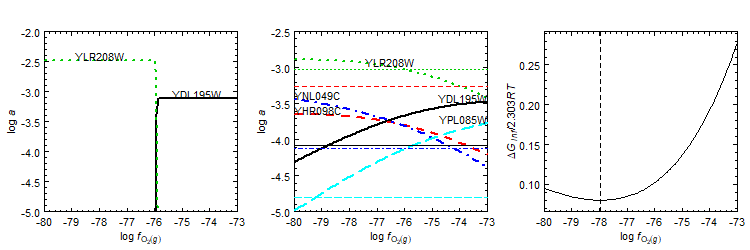
\includegraphics[width=0.85\linewidth]{anintro_chnosz_files/figure-latex/yeastplot-1} \caption[ER-to-Golgi proteins]{ER-to-Golgi proteins: calculations without and with length normalization, and free energy difference between experimental and calculated abundances in metastable equilibrium with normalization.}\label{fig:yeastplot}
\end{figure*}

The minimum free energy difference occurs near logfO2 = -78. This agrees
with the assessment shown in Figure 4 of \citet{Dic09} (note that the
old parameters for the methionine sidechain group were used in that
study).

\subsection{An affinity baseline}\label{an-affinity-baseline}

Because affinities of proteins often vary strongly with oxygen fugacity
and other variables, it can be helpful to express the values as
differences from a baseline. The following example compares the
affinities for formation of transcription factors involved in embryonic
dorsal-ventral patterning with that of the morphogen, Sonic hedgehog
(Shh), as a function of logfO2 and log\emph{a}H2O \citep{Dic15}. We
first list the UniProt names of Shh and 10 transcription factors, and
get the \texttt{iprotein} indices (rownumbers of
\texttt{thermo\$protein}):

\begin{Shaded}
\begin{Highlighting}[]
\NormalTok{pname <-}\StringTok{ }\KeywordTok{c}\NormalTok{(}\StringTok{"SHH"}\NormalTok{, }\StringTok{"OLIG2"}\NormalTok{, }\StringTok{"NKX22"}\NormalTok{, }\StringTok{"FOXA2"}\NormalTok{, }\StringTok{"IRX3"}\NormalTok{,}
  \StringTok{"PAX6"}\NormalTok{, }\StringTok{"NKX62"}\NormalTok{, }\StringTok{"DBX1"}\NormalTok{, }\StringTok{"DBX2"}\NormalTok{, }\StringTok{"NKX61"}\NormalTok{, }\StringTok{"PAX7"}\NormalTok{)}
\NormalTok{ip <-}\StringTok{ }\KeywordTok{pinfo}\NormalTok{(pname, }\StringTok{"HUMAN"}\NormalTok{)}
\end{Highlighting}
\end{Shaded}

Next, set up the basis species:

\begin{Shaded}
\begin{Highlighting}[]
\KeywordTok{basis}\NormalTok{(}\StringTok{"CHNOS"}\NormalTok{)}
\KeywordTok{basis}\NormalTok{(}\StringTok{"NH3"}\NormalTok{, }\OperatorTok{-}\DecValTok{7}\NormalTok{)}
\end{Highlighting}
\end{Shaded}

Now calculate the affinities of formation of the proteins from the basis
species. The values chosen for logfO2 and log\emph{a}H2O covary, so we
are using the transect mode of {\texttt{affinity()}}:

\begin{Shaded}
\begin{Highlighting}[]
\NormalTok{O2 <-}\StringTok{ }\KeywordTok{seq}\NormalTok{(}\OperatorTok{-}\DecValTok{70}\NormalTok{, }\OperatorTok{-}\DecValTok{106}\NormalTok{, }\DataTypeTok{length.out =} \DecValTok{50}\NormalTok{)}
\NormalTok{H2O <-}\StringTok{ }\KeywordTok{seq}\NormalTok{(}\FloatTok{0.5}\NormalTok{, }\OperatorTok{-}\FloatTok{5.5}\NormalTok{, }\DataTypeTok{length.out =} \DecValTok{50}\NormalTok{)}
\NormalTok{a <-}\StringTok{ }\KeywordTok{affinity}\NormalTok{(}\DataTypeTok{H2O =}\NormalTok{ H2O, }\DataTypeTok{O2 =}\NormalTok{ O2, }\DataTypeTok{iprotein =}\NormalTok{ ip)}
\end{Highlighting}
\end{Shaded}

We would like to compare the affinities of the proteins on a per-residue
scale. R's \texttt{lapply()} could be used here, but to show the
operation more clearly we use a \texttt{for()} loop:

\begin{Shaded}
\begin{Highlighting}[]
\NormalTok{pl <-}\StringTok{ }\KeywordTok{protein.length}\NormalTok{(ip)}
\ControlFlowTok{for}\NormalTok{(i }\ControlFlowTok{in} \KeywordTok{seq_along}\NormalTok{(a}\OperatorTok{$}\NormalTok{values)) a}\OperatorTok{$}\NormalTok{values[[i]] <-}\StringTok{ }\NormalTok{a}\OperatorTok{$}\NormalTok{values[[i]] }\OperatorTok{/}\StringTok{ }\NormalTok{pl[i]}
\end{Highlighting}
\end{Shaded}

Then, we calculate the relative affinities, using Shh as the baseline:

\begin{Shaded}
\begin{Highlighting}[]
\NormalTok{a.Shh <-}\StringTok{ }\NormalTok{a}\OperatorTok{$}\NormalTok{values[[}\DecValTok{1}\NormalTok{]]}
\ControlFlowTok{for}\NormalTok{(i }\ControlFlowTok{in} \DecValTok{1}\OperatorTok{:}\KeywordTok{length}\NormalTok{(a}\OperatorTok{$}\NormalTok{values)) a}\OperatorTok{$}\NormalTok{values[[i]] <-}\StringTok{ }\NormalTok{a}\OperatorTok{$}\NormalTok{values[[i]] }\OperatorTok{-}\StringTok{ }\NormalTok{a.Shh}
\end{Highlighting}
\end{Shaded}

Next we use {\texttt{diagram()}} to plot the affinities. We set
\texttt{balance\ =\ 1} to plot the values as they are---without that,
{\texttt{diagram()}} divides the values by protein length, which we have
already done!

\begin{marginfigure}
See \href{../demo}{{\texttt{demo(Shh)}}} for a plot with more
interpretive labels and comments.
\end{marginfigure}

For this plot, we highlight and label the proteins with the highest
relative affinity at some combination of logfO2 and log\emph{a}H2O along
the transect. Those proteins are Olig2, Irx3, Nkx6.2, Dbx1, and Shh
(numbers 2, 5, 7, 8, 1 in the set we have identified). Here,
\texttt{adj\ =\ 0} makes the labels left-aligned, \texttt{dy\ =\ 0.1}
adds a \emph{y} offset to the labels, and
\texttt{format.names\ =\ FALSE} prevents formatting of the names as if
they were chemical formulas (that causes subscripted numbers to appear).
The last few lines are used to make a second \emph{x} axis, using a
label generated with {\texttt{axis.label()}}:

\begin{marginfigure}
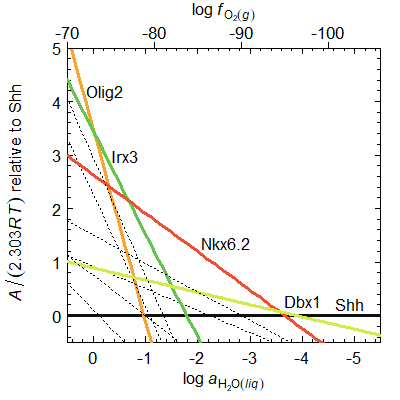
\includegraphics[width=1\linewidth]{anintro_chnosz_files/figure-latex/Shh_diagram-1} \caption[Per-residue affinities for formation of transcription factors relative to Shh]{Per-residue affinities for formation of transcription factors relative to Shh.}\label{fig:Shh_diagram}
\end{marginfigure}

\begin{Shaded}
\begin{Highlighting}[]
\CommentTok{# line type, width, and color}
\NormalTok{twc <-}\StringTok{ }\KeywordTok{lapply}\NormalTok{(}\KeywordTok{c}\NormalTok{(}\DecValTok{3}\NormalTok{, }\DecValTok{1}\NormalTok{, }\DecValTok{1}\NormalTok{), rep, }\KeywordTok{length}\NormalTok{(pname))}
\NormalTok{ihigh <-}\StringTok{ }\KeywordTok{c}\NormalTok{(}\DecValTok{2}\NormalTok{, }\DecValTok{5}\NormalTok{, }\DecValTok{7}\NormalTok{, }\DecValTok{8}\NormalTok{, }\DecValTok{1}\NormalTok{)}
\NormalTok{twc[[}\DecValTok{1}\NormalTok{]][ihigh] <-}\StringTok{ }\DecValTok{1}
\NormalTok{twc[[}\DecValTok{2}\NormalTok{]][ihigh] <-}\StringTok{ }\DecValTok{3}
\NormalTok{col <-}\StringTok{ }\KeywordTok{c}\NormalTok{(}\StringTok{"#f9a330"}\NormalTok{, }\StringTok{"#63c54e"}\NormalTok{, }\StringTok{"#f24e33"}\NormalTok{, }\StringTok{"#d4e94e"}\NormalTok{, }\StringTok{"#0f0f0f"}\NormalTok{)}
\NormalTok{twc[[}\DecValTok{3}\NormalTok{]][ihigh] <-}\StringTok{ }\NormalTok{col}
\NormalTok{names <-}\StringTok{ }\KeywordTok{rep}\NormalTok{(}\StringTok{""}\NormalTok{, }\KeywordTok{length}\NormalTok{(pname))}
\NormalTok{names[ihigh] <-}\StringTok{ }\KeywordTok{c}\NormalTok{(}\StringTok{"Olig2"}\NormalTok{, }\StringTok{"Irx3"}\NormalTok{, }\StringTok{"Nkx6.2"}\NormalTok{, }\StringTok{"Dbx1"}\NormalTok{, }\StringTok{"Shh"}\NormalTok{)}
\NormalTok{ylab <-}\StringTok{ }\KeywordTok{substitute}\NormalTok{(}\KeywordTok{italic}\NormalTok{(A) }\OperatorTok{/}\StringTok{ }\NormalTok{(}\FloatTok{2.303} \OperatorTok{*}\StringTok{ }\KeywordTok{italic}\NormalTok{(RT)) }\OperatorTok{*}\StringTok{ " relative to Shh"}\NormalTok{)}
\KeywordTok{diagram}\NormalTok{(a, }\DataTypeTok{balance =} \DecValTok{1}\NormalTok{, }\DataTypeTok{ylim =} \KeywordTok{c}\NormalTok{(}\OperatorTok{-}\FloatTok{0.5}\NormalTok{, }\DecValTok{5}\NormalTok{), }\DataTypeTok{xlim =} \KeywordTok{c}\NormalTok{(}\FloatTok{0.5}\NormalTok{, }\OperatorTok{-}\FloatTok{5.5}\NormalTok{),}
  \DataTypeTok{lty =}\NormalTok{ twc[[}\DecValTok{1}\NormalTok{]], }\DataTypeTok{lwd=}\NormalTok{twc[[}\DecValTok{2}\NormalTok{]], }\DataTypeTok{col =}\NormalTok{ twc[[}\DecValTok{3}\NormalTok{]], }\DataTypeTok{ylab =}\NormalTok{ ylab,}
  \DataTypeTok{names =}\NormalTok{ names, }\DataTypeTok{adj =} \DecValTok{0}\NormalTok{, }\DataTypeTok{dy =} \FloatTok{0.1}\NormalTok{, }\DataTypeTok{format.names =} \OtherTok{FALSE}\NormalTok{)}
\KeywordTok{par}\NormalTok{(}\DataTypeTok{usr =} \KeywordTok{c}\NormalTok{(}\OperatorTok{-}\DecValTok{70}\NormalTok{, }\OperatorTok{-}\DecValTok{106}\NormalTok{, }\OperatorTok{-}\FloatTok{0.5}\NormalTok{, }\DecValTok{5}\NormalTok{), }\DataTypeTok{tcl =} \OperatorTok{-}\FloatTok{0.3}\NormalTok{)}
\KeywordTok{axis}\NormalTok{(}\DecValTok{3}\NormalTok{, }\DataTypeTok{at =} \KeywordTok{seq}\NormalTok{(}\OperatorTok{-}\DecValTok{70}\NormalTok{, }\OperatorTok{-}\DecValTok{106}\NormalTok{, }\DataTypeTok{by =} \OperatorTok{-}\DecValTok{10}\NormalTok{))}
\KeywordTok{mtext}\NormalTok{(}\KeywordTok{axis.label}\NormalTok{(}\StringTok{"O2"}\NormalTok{), }\DataTypeTok{line =} \FloatTok{1.2}\NormalTok{)}
\end{Highlighting}
\end{Shaded}

Among these proteins, Olig2 and Shh have the greatest affinities for
formation at the extremes of oxidation and hydration state. This
thermodynamic description highlights possible links between the chemical
compositions of the proteins and their patterns of expression along with
chemical changes in developing embryos (Dick, 2015).

\subsection{Getting amino acid
compositions}\label{getting-amino-acid-compositions}

In the Rubisco example above, we saw the use of {\texttt{read.fasta()}}
to read amino acid sequences from a FASTA file. There are several other
methods for inputting amino acid compositions.

R's \texttt{read.csv()} can be used to read amino acid compositions from
a CSV file with the same columns that are present in
\texttt{thermo\$protein}. Note the use of \texttt{as.is\ =\ TRUE} to
prevent reading character data as factors. The \texttt{nrows} argument
can be added to read that number of rows:

\begin{Shaded}
\begin{Highlighting}[]
\NormalTok{file <-}\StringTok{ }\KeywordTok{system.file}\NormalTok{(}\StringTok{"extdata/protein/DS11.csv"}\NormalTok{, }\DataTypeTok{package =} \StringTok{"CHNOSZ"}\NormalTok{)}
\NormalTok{aa_bison <-}\StringTok{ }\KeywordTok{read.csv}\NormalTok{(file, }\DataTypeTok{as.is =} \OtherTok{TRUE}\NormalTok{, }\DataTypeTok{nrows =} \DecValTok{5}\NormalTok{)}
\end{Highlighting}
\end{Shaded}

{\texttt{yeast.aa()}} retrieves amino acid composition of proteins in
\emph{Saccharomyces cerevisiae} from a data file that is included with
CHNOSZ:

\begin{Shaded}
\begin{Highlighting}[]
\NormalTok{aa_YML020W <-}\StringTok{ }\KeywordTok{yeast.aa}\NormalTok{(}\StringTok{"YML020W"}\NormalTok{)}
\end{Highlighting}
\end{Shaded}

{\texttt{read.fasta()}} reads a FASTA file and returns the amino acid
compositions of the sequences. The \texttt{iseq} argument can be used to
read those sequences from the file:

\begin{Shaded}
\begin{Highlighting}[]
\NormalTok{file <-}\StringTok{ }\KeywordTok{system.file}\NormalTok{(}\StringTok{"extdata/fasta/EF-Tu.aln"}\NormalTok{, }\DataTypeTok{package =} \StringTok{"CHNOSZ"}\NormalTok{)}
\NormalTok{aa_Ef <-}\StringTok{ }\KeywordTok{read.fasta}\NormalTok{(file, }\DataTypeTok{iseq =} \DecValTok{1}\OperatorTok{:}\DecValTok{2}\NormalTok{)}
\end{Highlighting}
\end{Shaded}

{\texttt{seq2aa()}} counts the amino acids in a user-supplied sequence
and generates a data frame of the amino acid composition:

\begin{marginfigure}
See also {\texttt{?count.aa}}, which can process both protein and
nucleic acid sequences.
\end{marginfigure}

\begin{Shaded}
\begin{Highlighting}[]
\NormalTok{aa_PRIO <-}\StringTok{ }\KeywordTok{seq2aa}\NormalTok{(}\StringTok{"PRIO_HUMAN"}\NormalTok{, }\StringTok{"}
\StringTok{MANLGCWMLVLFVATWSDLGLCKKRPKPGGWNTGGSRYPGQGSPGGNRYPPQGGGGWGQP}
\StringTok{HGGGWGQPHGGGWGQPHGGGWGQPHGGGWGQGGGTHSQWNKPSKPKTNMKHMAGAAAAGA}
\StringTok{VVGGLGGYMLGSAMSRPIIHFGSDYEDRYYRENMHRYPNQVYYRPMDEYSNQNNFVHDCV}
\StringTok{NITIKQHTVTTTTKGENFTETDVKMMERVVEQMCITQYERESQAYYQRGSSMVLFSSPPV}
\StringTok{ILLISFLIFLIVG}
\StringTok{"}\NormalTok{)}
\end{Highlighting}
\end{Shaded}

{\texttt{uniprot.aa()}} returns the amino acid composition of a single
amino acid sequence downloaded from UniProt. To get sequences for many
proteins, use R's \texttt{lapply()}, \texttt{do.call()}, and
\texttt{rbind()}:

\begin{Shaded}
\begin{Highlighting}[]
\NormalTok{IDs <-}\StringTok{ }\KeywordTok{c}\NormalTok{(}\StringTok{"ALAT1_HUMAN"}\NormalTok{, }\StringTok{"P02452"}\NormalTok{)}
\NormalTok{aa <-}\StringTok{ }\KeywordTok{lapply}\NormalTok{(IDs, uniprot.aa)}
\NormalTok{## uniprot.aa: trying http://www.uniprot.org/uniprot/ALAT1_HUMAN ... accession P24298 ...}
\NormalTok{## >sp|P24298|ALAT1_HUMAN Alanine aminotransferase 1 OS=Homo sapiens GN=GPT PE=1 SV=3 (length 496)}
\NormalTok{## uniprot.aa: trying http://www.uniprot.org/uniprot/P02452 ... accession P02452 ...}
\NormalTok{## >sp|P02452|CO1A1_HUMAN Collagen alpha-1(I) chain OS=Homo sapiens GN=COL1A1 PE=1 SV=5 (length 1464)}
\NormalTok{aa_UniProt <-}\StringTok{ }\KeywordTok{do.call}\NormalTok{(rbind, aa)}
\end{Highlighting}
\end{Shaded}

\begin{Shaded}
\begin{Highlighting}[]
\NormalTok{aa_UniProt}
\end{Highlighting}
\end{Shaded}

\begin{verbatim}
##      protein organism ref abbrv chains Ala Cys Asp Glu Phe Gly His Ile Lys Leu
## 1  sp|P24298    HUMAN  NA ALAT1      1  51  10  20  34  21  38   9  18  16  55
## 11 sp|P02452    HUMAN  NA CO1A1      1 139  18  66  75  27 391   9  24  57  48
##    Met Asn Pro Gln Arg Ser Thr Val Trp Tyr
## 1   12  12  33  30  37  25  18  41   1  15
## 11  13  28 278  49  71  60  45  47   6  13
\end{verbatim}

These amino acid compositions can be processed using functions such as
{\texttt{protein.length()}} and {\texttt{protein.formula()}}:

\begin{Shaded}
\begin{Highlighting}[]
\NormalTok{myaa <-}\StringTok{ }\KeywordTok{rbind}\NormalTok{(aa_YML020W, aa_Ef, aa_PRIO)}
\KeywordTok{protein.length}\NormalTok{(myaa)}
\end{Highlighting}
\end{Shaded}

\begin{verbatim}
## [1] 664 394 394 253
\end{verbatim}

\subsection{\texorpdfstring{Adding proteins and using
\texttt{iprotein}}{Adding proteins and using iprotein}}\label{adding-proteins-and-using-iprotein}

Once the amino acid compositions have been obtained, use
{\texttt{add.protein()}} to add these proteins to
\texttt{thermo\$protein}:

\begin{Shaded}
\begin{Highlighting}[]
\KeywordTok{add.protein}\NormalTok{(myaa)}
\end{Highlighting}
\end{Shaded}

\begin{verbatim}
## [1] 512 513 514 515
\end{verbatim}

Then, {\texttt{subcrt()}} can be used to calculate the standard
thermodynamic properties of any of these proteins:

\begin{Shaded}
\begin{Highlighting}[]
\KeywordTok{subcrt}\NormalTok{(}\StringTok{"PRIO_HUMAN"}\NormalTok{, }\DataTypeTok{T =} \DecValTok{25}\NormalTok{)}
\end{Highlighting}
\end{Shaded}

\begin{verbatim}
## $species
##            name               formula state ispecies
## 3618 PRIO_HUMAN C1227H1834N352O352S16    aq     3618
## 
## $out
## $out$PRIO_HUMAN
##    T P      rho    logK        G         H       S       V      Cp
## 1 25 1 0.997061 5486.45 -7484855 -19116027 8124.78 20084.3 12174.4
\end{verbatim}

Or we can add any of these proteins to the species list with
{\texttt{species()}} and calculate the affinity:

\begin{Shaded}
\begin{Highlighting}[]
\KeywordTok{basis}\NormalTok{(}\StringTok{"CHNOS"}\NormalTok{)}
\end{Highlighting}
\end{Shaded}

\begin{Shaded}
\begin{Highlighting}[]
\KeywordTok{species}\NormalTok{(}\StringTok{"YML020W_Sce"}\NormalTok{)}
\end{Highlighting}
\end{Shaded}

\begin{verbatim}
##    CO2  H2O NH3 H2S    O2 ispecies logact state        name
## 1 3406 1247 932  13 -3517     3619     -3    aq YML020W_Sce
\end{verbatim}

\begin{Shaded}
\begin{Highlighting}[]
\NormalTok{a <-}\StringTok{ }\KeywordTok{affinity}\NormalTok{()}
\end{Highlighting}
\end{Shaded}

Or we can calculate the affinities of formation reactions of the
proteins without adding them as species:

\begin{Shaded}
\begin{Highlighting}[]
\NormalTok{ip <-}\StringTok{ }\KeywordTok{add.protein}\NormalTok{(aa_UniProt)}
\NormalTok{a <-}\StringTok{ }\KeywordTok{affinity}\NormalTok{(}\DataTypeTok{iprotein =}\NormalTok{ ip)}
\end{Highlighting}
\end{Shaded}

As shown there, the \texttt{iprotein} argument of {\texttt{affinity()}}
can be used to calculate the affinities of reactions to form the
indicated proteins, bypassing the {\texttt{species()}} step. Let's see
this in action using amino acid compositions deduced from metagenomic
sequences in the Bison Pool hot spring in Yellowstone \citep{DS11}. We
read a data file of amino acid compositions produced in that study,
taking those labeled ``transferase''. Then we add the proteins and get
their indices using {\texttt{add.protein()}}, set the basis, calculate
the affinities, and make a potential diagram with temperature and
activity of dissolved hydrogen as variables:

\begin{marginfigure}
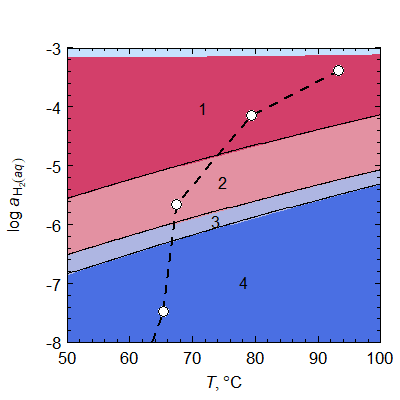
\includegraphics[width=1\linewidth]{anintro_chnosz_files/figure-latex/bison_transferase-1} \caption[Potential diagram for metagenomically identified sequences of transferases in Bison Pool hot spring]{Potential diagram for metagenomically identified sequences of transferases in Bison Pool hot spring. See also the vignette [<span style="color:blue">*Hot-spring proteins in CHNOSZ*</span>](hotspring.pdf).}\label{fig:bison_transferase}
\end{marginfigure}

\begin{Shaded}
\begin{Highlighting}[]
\NormalTok{file <-}\StringTok{ }\KeywordTok{system.file}\NormalTok{(}\StringTok{"extdata/protein/DS11.csv"}\NormalTok{, }\DataTypeTok{package =} \StringTok{"CHNOSZ"}\NormalTok{)}
\NormalTok{aa <-}\StringTok{ }\KeywordTok{read.csv}\NormalTok{(file, }\DataTypeTok{as.is =} \OtherTok{TRUE}\NormalTok{)}
\NormalTok{aa <-}\StringTok{ }\NormalTok{aa[}\KeywordTok{grep}\NormalTok{(}\StringTok{"transferase"}\NormalTok{, aa}\OperatorTok{$}\NormalTok{protein), ]}
\NormalTok{ip <-}\StringTok{ }\KeywordTok{add.protein}\NormalTok{(aa)}
\KeywordTok{basis}\NormalTok{(}\KeywordTok{c}\NormalTok{(}\StringTok{"HCO3-"}\NormalTok{, }\StringTok{"H2O"}\NormalTok{, }\StringTok{"NH3"}\NormalTok{, }\StringTok{"HS-"}\NormalTok{, }\StringTok{"H2"}\NormalTok{, }\StringTok{"H+"}\NormalTok{))}
\KeywordTok{basis}\NormalTok{(}\KeywordTok{c}\NormalTok{(}\StringTok{"HCO3-"}\NormalTok{, }\StringTok{"NH3"}\NormalTok{, }\StringTok{"HS-"}\NormalTok{, }\StringTok{"H+"}\NormalTok{), }\KeywordTok{c}\NormalTok{(}\OperatorTok{-}\DecValTok{3}\NormalTok{, }\OperatorTok{-}\DecValTok{4}\NormalTok{, }\OperatorTok{-}\DecValTok{7}\NormalTok{, }\OperatorTok{-}\FloatTok{7.9}\NormalTok{))}
\NormalTok{T <-}\StringTok{ }\KeywordTok{c}\NormalTok{(}\DecValTok{50}\NormalTok{, }\DecValTok{100}\NormalTok{)}
\NormalTok{res <-}\StringTok{ }\DecValTok{300}
\NormalTok{a <-}\StringTok{ }\KeywordTok{affinity}\NormalTok{(}\DataTypeTok{T =} \KeywordTok{c}\NormalTok{(T, res), }\DataTypeTok{H2 =} \KeywordTok{c}\NormalTok{(}\OperatorTok{-}\DecValTok{8}\NormalTok{, }\OperatorTok{-}\DecValTok{3}\NormalTok{, res), }\DataTypeTok{iprotein =}\NormalTok{ ip)}
\NormalTok{fill <-}\StringTok{ }\KeywordTok{ZC.col}\NormalTok{(}\KeywordTok{ZC}\NormalTok{(}\KeywordTok{protein.formula}\NormalTok{(ip)))}
\KeywordTok{diagram}\NormalTok{(a, }\DataTypeTok{normalize =} \OtherTok{TRUE}\NormalTok{, }\DataTypeTok{fill =}\NormalTok{ fill, }\DataTypeTok{names =} \DecValTok{1}\OperatorTok{:}\DecValTok{5}\NormalTok{)}
\end{Highlighting}
\end{Shaded}

Site numbers 1--5 correspond to a cooling gradient along the outflow
channel of the hot spring. The colors represent the relative ZC of the
proteins (red is more reduced). The points indicate the \emph{T} and
log\emph{a}H2 that optimize a thermodynamic model for relative
abundances of phyla that were estimated by taxonomic classification of
metagenomic sequences \citep{DS13}:

\begin{Shaded}
\begin{Highlighting}[]
\NormalTok{T <-}\StringTok{ }\KeywordTok{c}\NormalTok{(}\FloatTok{93.3}\NormalTok{, }\FloatTok{79.4}\NormalTok{, }\FloatTok{67.5}\NormalTok{, }\FloatTok{65.3}\NormalTok{, }\FloatTok{57.1}\NormalTok{)}
\NormalTok{logaH2 <-}\StringTok{ }\KeywordTok{c}\NormalTok{(}\OperatorTok{-}\FloatTok{3.38}\NormalTok{, }\OperatorTok{-}\FloatTok{4.14}\NormalTok{, }\OperatorTok{-}\FloatTok{5.66}\NormalTok{, }\OperatorTok{-}\FloatTok{7.47}\NormalTok{, }\OperatorTok{-}\FloatTok{10.02}\NormalTok{)}
\KeywordTok{lines}\NormalTok{(T, logaH2, }\DataTypeTok{lty =} \DecValTok{2}\NormalTok{, }\DataTypeTok{lwd =} \DecValTok{2}\NormalTok{)}
\KeywordTok{points}\NormalTok{(T, logaH2, }\DataTypeTok{pch =} \DecValTok{21}\NormalTok{, }\DataTypeTok{bg =} \StringTok{"white"}\NormalTok{, }\DataTypeTok{cex =} \FloatTok{1.5}\NormalTok{)}
\end{Highlighting}
\end{Shaded}

\hypertarget{optimization-of-chemical-activities}{\section{Optimization
of chemical activities}\label{optimization-of-chemical-activities}}

\textbf{NOTE: This is an experimental feature.}

What are the conditions that minimize the standard deviation of
calculated activities of species? What are the conditions that minimize
the energetic difference between measured and calculated abundances?
These are questions about optimization of chemical activities.
{\texttt{revisit()}} provides calculations and plots of an objective
function in 1 or 2 dimensions (activities of basis species, \emph{T}, or
\emph{P}).

\begin{marginfigure}
See {\texttt{?objective}} for more information.
\end{marginfigure}

{\texttt{findit()}} provides a calculation of an objective function on a
higher-dimensional grid.

The concentrations of amino acids are affected by high-temperature
reactions in hydrothermal vents (smokers). What are the metastable
equilibrium states of amino acids under these conditions? Suppose that
the major variables are oxygen fugacity, and activities of water (H2O)
and ammonia (NH3). Here we assign the (very large) range of logarithms
of chemical activity of the basis species that we will explore:

\begin{Shaded}
\begin{Highlighting}[]
\NormalTok{vars <-}\StringTok{ }\KeywordTok{list}\NormalTok{(}\DataTypeTok{O2 =} \KeywordTok{c}\NormalTok{(}\OperatorTok{-}\DecValTok{50}\NormalTok{, }\OperatorTok{-}\DecValTok{25}\NormalTok{), }\DataTypeTok{NH3 =} \KeywordTok{c}\NormalTok{(}\OperatorTok{-}\DecValTok{15}\NormalTok{, }\DecValTok{10}\NormalTok{), }\DataTypeTok{H2O =} \KeywordTok{c}\NormalTok{(}\OperatorTok{-}\DecValTok{15}\NormalTok{, }\DecValTok{10}\NormalTok{))}
\end{Highlighting}
\end{Shaded}

Consider the amino acid abundances reported by \citet{FMM_14}. Here, we
identify the amino acids using their one-letter abbreviations. Then,
{\texttt{aminoacids()}} is used to produce the full names, which in turn
are used to search \texttt{thermo\$obigt} for their formulas.
{\texttt{makeup()}} is used to count the elements in the formulas:

\begin{Shaded}
\begin{Highlighting}[]
\NormalTok{aa <-}\StringTok{ }\KeywordTok{c}\NormalTok{(}\StringTok{"D"}\NormalTok{, }\StringTok{"T"}\NormalTok{, }\StringTok{"S"}\NormalTok{, }\StringTok{"E"}\NormalTok{, }\StringTok{"G"}\NormalTok{, }\StringTok{"A"}\NormalTok{, }\StringTok{"K"}\NormalTok{, }\StringTok{"H"}\NormalTok{)}
\NormalTok{AA <-}\StringTok{ }\KeywordTok{aminoacids}\NormalTok{(}\StringTok{""}\NormalTok{, aa)}
\NormalTok{AA.formula <-}\StringTok{ }\KeywordTok{do.call}\NormalTok{(rbind, }\KeywordTok{makeup}\NormalTok{(}\KeywordTok{info}\NormalTok{(AA)))}
\NormalTok{AA}
\end{Highlighting}
\end{Shaded}

\begin{verbatim}
## [1] "aspartic acid" "threonine"     "serine"        "glutamic acid"
## [5] "glycine"       "alanine"       "lysine"        "histidine"
\end{verbatim}

Let's use the reported concentrations (µM) of amino acids in sample
D1441 CW-2.

\begin{marginfigure}
Three amino acids (Val, Phe, Arg) with concentrations below the
detection limit of 0.01 µM are not included here.
\end{marginfigure}

The concentrations are converted to logarithmic values (\texttt{loga2}).
We then calculate the total C concentration in the measurements; this
uses the amino acid formulas calculated above:

\begin{Shaded}
\begin{Highlighting}[]
\NormalTok{uM <-}\StringTok{ }\KeywordTok{c}\NormalTok{(}\FloatTok{1.10}\NormalTok{, }\FloatTok{0.70}\NormalTok{, }\FloatTok{3.73}\NormalTok{, }\FloatTok{0.39}\NormalTok{, }\FloatTok{3.04}\NormalTok{, }\FloatTok{1.83}\NormalTok{, }\FloatTok{0.27}\NormalTok{, }\FloatTok{0.21}\NormalTok{)}
\NormalTok{loga2 <-}\StringTok{ }\KeywordTok{log10}\NormalTok{(uM }\OperatorTok{*}\StringTok{ }\FloatTok{1e-6}\NormalTok{)}
\NormalTok{nC <-}\StringTok{ }\NormalTok{AA.formula[, }\StringTok{"C"}\NormalTok{]}
\NormalTok{Ctot <-}\StringTok{ }\KeywordTok{sum}\NormalTok{(nC }\OperatorTok{*}\StringTok{ }\NormalTok{uM }\OperatorTok{*}\StringTok{ }\FloatTok{1e-6}\NormalTok{)}
\end{Highlighting}
\end{Shaded}

Next, we set the basis, load the species, and assign the temperature and
resolution to be used in {\texttt{affinity()}}. Also, we assign the
objective function to be the root mean square deviation (RMSD) between
experimental and calculated logarithms:

\begin{Shaded}
\begin{Highlighting}[]
\KeywordTok{basis}\NormalTok{(}\StringTok{"CHNOS"}\NormalTok{)}
\KeywordTok{species}\NormalTok{(AA)}
\NormalTok{T <-}\StringTok{ }\DecValTok{270}
\NormalTok{res <-}\StringTok{ }\DecValTok{64}
\NormalTok{objective <-}\StringTok{ "RMSD"}
\end{Highlighting}
\end{Shaded}

Then, we set up the figure, calculate chemical affinities in one
dimension, and run {\texttt{equilibrate()}} with the given total carbon
activity. {\texttt{revisit()}} is used to plot RMSD and to identify the
logfO2 where it is minimized:

\begin{Shaded}
\begin{Highlighting}[]
\KeywordTok{layout}\NormalTok{(}\KeywordTok{matrix}\NormalTok{(}\DecValTok{1}\OperatorTok{:}\DecValTok{6}\NormalTok{, }\DataTypeTok{nrow =} \DecValTok{2}\NormalTok{))}
\NormalTok{a <-}\StringTok{ }\KeywordTok{affinity}\NormalTok{(}\DataTypeTok{O2 =} \KeywordTok{c}\NormalTok{(vars[[}\DecValTok{1}\NormalTok{]], res), }\DataTypeTok{T =}\NormalTok{ T)}
\NormalTok{e <-}\StringTok{ }\KeywordTok{equilibrate}\NormalTok{(a, }\DataTypeTok{loga.balance =} \KeywordTok{log10}\NormalTok{(Ctot))}
\NormalTok{r <-}\StringTok{ }\KeywordTok{revisit}\NormalTok{(e, objective, loga2)}
\NormalTok{d.basis <-}\StringTok{ }\KeywordTok{describe.basis}\NormalTok{(}\DataTypeTok{ibasis =} \DecValTok{1}\OperatorTok{:}\DecValTok{4}\NormalTok{)}
\KeywordTok{legend}\NormalTok{(}\StringTok{"topleft"}\NormalTok{, d.basis)}
\end{Highlighting}
\end{Shaded}

Now, we write a function that calculates the affinities and metastable
equilibrium activities at a single condition and uses
{\texttt{revisit()}} to make a scatter plot. The plot includes a 1:1
line (grey), a trend line calculated using R's \texttt{loess.smooth()}
(red), and a title with the minimum value of RMSD. The function also
adds a legend summarizing the optimal conditions:

\begin{Shaded}
\begin{Highlighting}[]
\NormalTok{ourfun <-}\StringTok{ }\ControlFlowTok{function}\NormalTok{(}\DataTypeTok{ibasis =} \DecValTok{1}\OperatorTok{:}\DecValTok{5}\NormalTok{, }\DataTypeTok{x =} \StringTok{"bottomright"}\NormalTok{) \{}
\NormalTok{  a <-}\StringTok{ }\KeywordTok{affinity}\NormalTok{(}\DataTypeTok{T =}\NormalTok{ T)}
\NormalTok{  e <-}\StringTok{ }\KeywordTok{equilibrate}\NormalTok{(a, }\DataTypeTok{loga.balance =} \KeywordTok{log10}\NormalTok{(Ctot))}
  \KeywordTok{revisit}\NormalTok{(e, objective, loga2, }\DataTypeTok{cex =} \FloatTok{2.7}\NormalTok{, }\DataTypeTok{pch =} \DecValTok{21}\NormalTok{)}
  \KeywordTok{text}\NormalTok{(loga2, }\KeywordTok{unlist}\NormalTok{(e}\OperatorTok{$}\NormalTok{loga.equil), aa)}
\NormalTok{  d.basis <-}\StringTok{ }\KeywordTok{describe.basis}\NormalTok{(}\DataTypeTok{ibasis =}\NormalTok{ ibasis)}
  \KeywordTok{legend}\NormalTok{(x, d.basis)}
\NormalTok{\}}
\end{Highlighting}
\end{Shaded}

We set the activity of logfO2 in the basis (where RMSD was minimized the
first call to {\texttt{revisit()}}), then use our function to make a
scatter plot:

\begin{Shaded}
\begin{Highlighting}[]
\KeywordTok{basis}\NormalTok{(}\StringTok{"O2"}\NormalTok{, r}\OperatorTok{$}\NormalTok{xopt)}
\KeywordTok{ourfun}\NormalTok{(}\DecValTok{5}\NormalTok{)}
\end{Highlighting}
\end{Shaded}

In the next pair of plots, let's use two variables: logfO2 and
log\emph{a}NH3. This time, {\texttt{revisit()}} makes a contour diagram
of the objective function, highlighting the location of the minimum
(star) as well as the minimum trough following the \emph{x} or \emph{y}
axis (dotted blue and green lines). After that, we set the activities of
both of the basis species and then use \texttt{ourfun()} to make a
scatter plot. The legend here shows the two variables that have been
optimized; these conditions yield an RMSD that is lower than in the
first calculation:

\begin{Shaded}
\begin{Highlighting}[]
\NormalTok{a <-}\StringTok{ }\KeywordTok{affinity}\NormalTok{(}\DataTypeTok{O2 =} \KeywordTok{c}\NormalTok{(vars[[}\DecValTok{1}\NormalTok{]], res), }\DataTypeTok{NH3 =} \KeywordTok{c}\NormalTok{(vars[[}\DecValTok{2}\NormalTok{]], res), }\DataTypeTok{T =}\NormalTok{ T)}
\NormalTok{e <-}\StringTok{ }\KeywordTok{equilibrate}\NormalTok{(a, }\DataTypeTok{loga.balance =} \KeywordTok{log10}\NormalTok{(Ctot))}
\NormalTok{r <-}\StringTok{ }\KeywordTok{revisit}\NormalTok{(e, objective, loga2)}
\KeywordTok{basis}\NormalTok{(}\StringTok{"O2"}\NormalTok{, r}\OperatorTok{$}\NormalTok{xopt)}
\KeywordTok{basis}\NormalTok{(}\StringTok{"NH3"}\NormalTok{, r}\OperatorTok{$}\NormalTok{yopt)}
\KeywordTok{ourfun}\NormalTok{(}\KeywordTok{c}\NormalTok{(}\DecValTok{3}\NormalTok{, }\DecValTok{5}\NormalTok{))}
\end{Highlighting}
\end{Shaded}

Finally, we use {\texttt{findit()}} to optimize three variables. The
affinity and equilibrium calculations are integrated into
{\texttt{findit()}}, so the function call requires the
\texttt{loga.balance} and \texttt{T} arguments. Other arguments indicate
the grid resolution, factor (ratio) by which variable ranges are reduced
in each step, and the number of iterations. The result is a series of 2D
contour plots of decreasing range, each one constructed for the optimal
value of log\emph{a}H2O from the previous step.

\begin{marginfigure}
More dimensions require a lower resolution due to limited computational
resources.
\end{marginfigure}

While running, {\texttt{findit()}} sets the activities of basis species,
so we can immediately call \texttt{ourfun()} to make make a scatter
plot.

\begin{marginfigure}
This side effect (changing the activities of basis species) is why the
text for {\texttt{findit()}} is colored red.
\end{marginfigure}

\begin{Shaded}
\begin{Highlighting}[]
\KeywordTok{findit}\NormalTok{(vars[}\DecValTok{1}\OperatorTok{:}\DecValTok{3}\NormalTok{], objective, }\DataTypeTok{loga2 =}\NormalTok{ loga2, }\DataTypeTok{loga.balance =} \KeywordTok{log10}\NormalTok{(Ctot),}
       \DataTypeTok{T =}\NormalTok{ T, }\DataTypeTok{res =} \DecValTok{8}\NormalTok{, }\DataTypeTok{niter =} \DecValTok{3}\NormalTok{, }\DataTypeTok{rat =} \FloatTok{0.6}\NormalTok{)}
\KeywordTok{ourfun}\NormalTok{(}\KeywordTok{c}\NormalTok{(}\DecValTok{2}\NormalTok{, }\DecValTok{3}\NormalTok{, }\DecValTok{5}\NormalTok{), }\StringTok{"right"}\NormalTok{)}
\end{Highlighting}
\end{Shaded}

\begin{figure*}
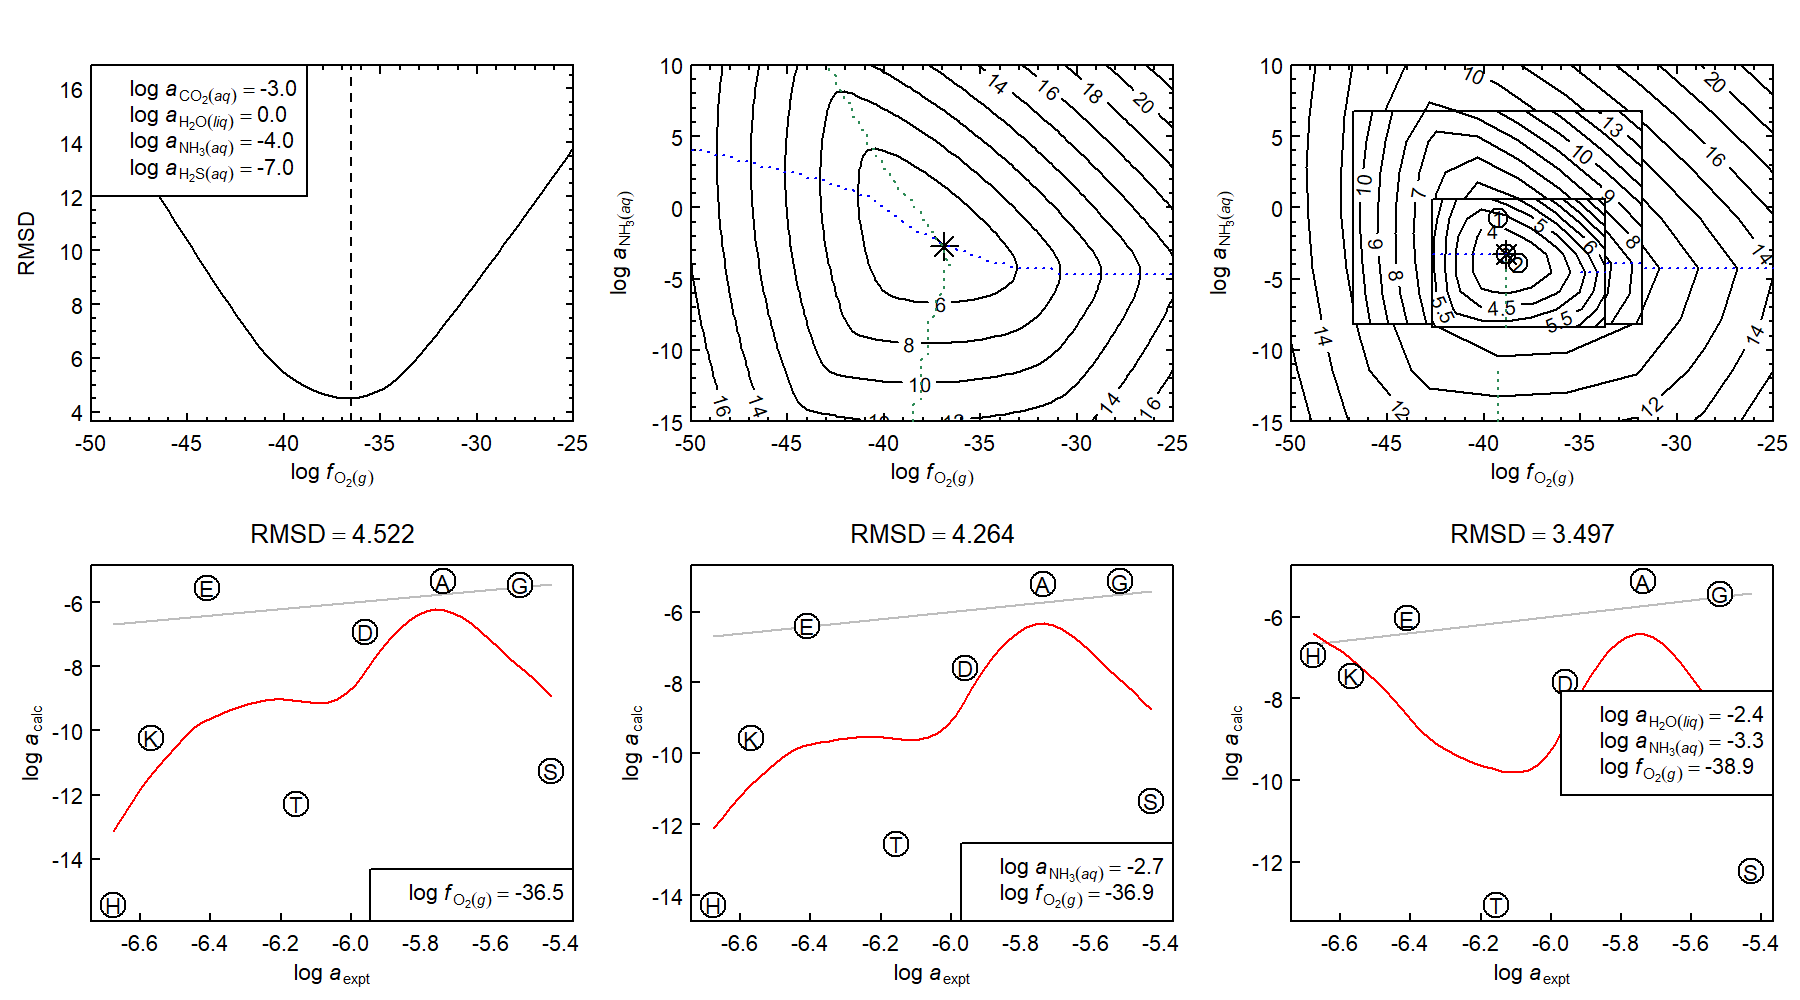
\includegraphics[width=0.85\linewidth]{anintro_chnosz_files/figure-latex/smoker_plot-1} \caption[Optimization of a thermodynamic model for relative abundances of amino acids in a 270 °C black smoker fluid using 1, 2, or 3 variables (left to right)]{Optimization of a thermodynamic model for relative abundances of amino acids in a 270 °C black smoker fluid using 1, 2, or 3 variables (left to right).}\label{fig:smoker_plot}
\end{figure*}

The calculation using {\texttt{findit()}}, in which the added variable
log\emph{a}H2O optimizes to ca. -2.4, shows that measured concentrations
of 6 amino acids fall within 1--2 log units of the relative abundances
in metastable equilibrium. According these calculations, two amino
acids, serine and threonine, are very far from metastable equilibrium
with the others. There is a danger of using too many, or
unrepresentative variables, but in some systems, calculations of this
type may provide insight on processes affecting reactions of organic
compounds.

\section{Thermodynamic data}\label{thermodynamic-data}

\subsection{\texorpdfstring{Viewing data sources:
{\texttt{thermo.refs()}}}{Viewing data sources: thermo.refs()}}\label{viewing-data-sources-thermo.refs}

The database in CHNOSZ lists one or two sources for each entry, and
citation information for the sources is listed in \texttt{thermo\$refs}.
You can locate and view the references with {\texttt{thermo.refs()}}.
Running the function without any arguments opens a browser window with
the complete table of references.

\begin{marginfigure}
See the vignette, \href{obigt.html}{{\emph{Thermodynamic data in
CHNOSZ}}}, for a more nicely formatted presentation of the sources of
thermodynamic data, along with notes and additional comments.
\end{marginfigure}

Where available, links to the web page for the articles and books are
displayed:

\begin{Shaded}
\begin{Highlighting}[]
\KeywordTok{thermo.refs}\NormalTok{()  ## shows table in a browser}
\end{Highlighting}
\end{Shaded}

A numeric argument to {\texttt{thermo.refs()}} gives one or more species
indices for which to get the references:

\begin{Shaded}
\begin{Highlighting}[]
\NormalTok{iATP <-}\StringTok{ }\KeywordTok{info}\NormalTok{(}\StringTok{"ATP-4"}\NormalTok{)}
\NormalTok{iMgATP <-}\StringTok{ }\KeywordTok{info}\NormalTok{(}\StringTok{"MgATP-2"}\NormalTok{)}
\KeywordTok{thermo.refs}\NormalTok{(}\KeywordTok{c}\NormalTok{(iATP, iMgATP))}
\end{Highlighting}
\end{Shaded}

\begin{verbatim}
##       key                          author year                               citation                                                    note
## 99  LH06a D. E. LaRowe and H. C. Helgeson 2006 Geochim. Cosmochim. Acta 70, 4680-4724        nucleic-acid bases, nucleosides, and nucleotides
## 101 LH06b D. E. LaRowe and H. C. Helgeson 2006           Thermochim. Acta 448, 82-106 Mg-complexed adenosine nucleotides (ATP), NAD, and NADP
##                                           URL
## 99  https://doi.org/10.1016/j.gca.2006.04.010
## 101 https://doi.org/10.1016/j.tca.2006.06.008
\end{verbatim}

A character argument gives the source key(s):

\begin{Shaded}
\begin{Highlighting}[]
\KeywordTok{thermo.refs}\NormalTok{(}\KeywordTok{c}\NormalTok{(}\StringTok{"HDNB78"}\NormalTok{, }\StringTok{"MGN03"}\NormalTok{))}
\end{Highlighting}
\end{Shaded}

\begin{verbatim}
##       key                                    author year                 citation                                              note                                   URL
## 8  HDNB78       H. C. Helgeson, J. M. Delany et al. 1978  Am. J. Sci. 278A, 1-229 data for minerals (n = 167) and phase transitions http://www.worldcat.org/oclc/13594862
## 90  MGN03 J. Majzlan, K.-D. Grevel and A. Navrotsky 2003 Am. Mineral. 88, 855-859        goethite, lepidocrocite, and maghemite GHS https://doi.org/10.2138/am-2003-5-614
\end{verbatim}

If the argument holds the result of {\texttt{subcrt()}}, references for
all species in the reaction are returned:

\begin{marginfigure}
The exception is H2O. With the default settings, thermodynamic
properties for H2O are derived from SUPCRT92 (Johnson et al., 1992).
\end{marginfigure}

\begin{Shaded}
\begin{Highlighting}[]
\NormalTok{substuff <-}\StringTok{ }\KeywordTok{subcrt}\NormalTok{(}\KeywordTok{c}\NormalTok{(}\StringTok{"C2H5OH"}\NormalTok{, }\StringTok{"O2"}\NormalTok{, }\StringTok{"CO2"}\NormalTok{, }\StringTok{"H2O"}\NormalTok{), }\KeywordTok{c}\NormalTok{(}\OperatorTok{-}\DecValTok{1}\NormalTok{, }\OperatorTok{-}\DecValTok{3}\NormalTok{, }\DecValTok{2}\NormalTok{, }\DecValTok{3}\NormalTok{))}
\KeywordTok{thermo.refs}\NormalTok{(substuff)}
\end{Highlighting}
\end{Shaded}

\begin{verbatim}
##      key                                           author year                               citation                      note                                           URL
## 84  PS01                  A. V. Plyasunov and E. L. Shock 2001 Geochim. Cosmochim. Acta 65, 3879-3900   aqueous nonelectrolytes https://doi.org/10.1016/S0016-7037(01)00678-0
## 23 SHS89 E. L. Shock, H. C. Helgeson and D. A. Sverjensky 1989 Geochim. Cosmochim. Acta 53, 2157-2183 inorganic neutral species  https://doi.org/10.1016/0016-7037(89)90341-4
\end{verbatim}

The URLs of the references can be copied to a browser, or opened using
R's \texttt{browseURL()}:

\begin{Shaded}
\begin{Highlighting}[]
\NormalTok{iFo <-}\StringTok{ }\KeywordTok{info}\NormalTok{(}\StringTok{"forsterite"}\NormalTok{)}
\NormalTok{ref <-}\StringTok{ }\KeywordTok{thermo.refs}\NormalTok{(iFo)}
\KeywordTok{browseURL}\NormalTok{(ref}\OperatorTok{$}\NormalTok{URL)  ## opens a link to worldcat.org}
\end{Highlighting}
\end{Shaded}

\hypertarget{optional-data}{\subsection{Optional
data}\label{optional-data}}

Thermodynamic properties of minerals in the default database are mostly
taken from \citet{HDNB78}. These are identified by the state
\texttt{cr}, and \texttt{cr2}, \texttt{cr3}, etc. for higher-temperature
polymorphs. Optionally, thermodynamic properties of minerals can be
calculated using the equations and dataset of \citet{Ber88}; these
minerals are identified in the database by having the state
\texttt{cr\_Berman}.

Two other optional datasets can be activated by using
{\texttt{add.obigt()}}:

{\texttt{add.obigt("SUPCRTBL")}} -- This loads updated thermodynamic
parameters for aqueous SiO2, aluminum and arsenic species, and minerals,
as compiled in the
\href{http://www.indiana.edu/~hydrogeo/supcrtbl.html}{SUPCRTBL package}
\citep{ZZL_16}. SUPCRTBL also includes modifications to SUPCRT92 for
calculating thermodynamic properties of minerals using the \citet{HP11}
dataset, but that is not available in CHNOSZ. Instead, the Berman
mineral data can be used with similar results; see
\href{../demo}{{\texttt{demo(go-IU)}}}.

{\texttt{add.obigt("DEW")}} -- These are aqueous species, with modified
parameters, that are intended for use with the
\href{http://www.dewcommunity.org/}{Deep Earth Water} (DEW) model
\citep{SHA14}. You should also run {\texttt{water("DEW")}} to activate
the equations in the model; then, they will be used by
{\texttt{subcrt()}} and {\texttt{affinity()}}. Examples are in
\href{../demo}{{\texttt{demo(DEW)}}}.

Detailed lists of sources for these Optional Data are in the vignette
\href{obigt.html}{{\emph{Thermodynamic data in CHNOSZ}}} (look under
\textbf{Solids} / \textbf{Berman}, \textbf{Optional Data} /
\textbf{SUPCRTBL} and \textbf{Optional Data} / \textbf{DEW}).

\hypertarget{adding-data}{\subsection{Adding data}\label{adding-data}}

You can also use {\texttt{add.obigt()}} to add data from a
user-specified file to the database in the current session. The file
must be a CSV (comma separated value) file with column headers that
match those in the main database. To show the required format, take a
look at \texttt{BZA10.csv}, a supplemental data file provided in CHNOSZ.
Missing values are indicated by \texttt{NA}:

\begin{marginfigure}
R's \texttt{read.csv()} has a useful option: \texttt{as.is\ =\ TRUE}.
This prevents columns with character data from being read as factors
(i.e.~categorical data). Passing factors to functions that are designed
for character data can give unexpected results or errors.
\end{marginfigure}

\begin{Shaded}
\begin{Highlighting}[]
\NormalTok{file <-}\StringTok{ }\KeywordTok{system.file}\NormalTok{(}\StringTok{"extdata/thermo/BZA10.csv"}\NormalTok{, }\DataTypeTok{package =} \StringTok{"CHNOSZ"}\NormalTok{)}
\KeywordTok{read.csv}\NormalTok{(file, }\DataTypeTok{as.is =} \OtherTok{TRUE}\NormalTok{)}
\end{Highlighting}
\end{Shaded}

\begin{verbatim}
##      name abbrv formula state  ref1 ref2      date       G  H     S     Cp
## 1   CdCl+    NA   CdCl+    aq BZA10   NA 03.Jul.10  -52629 NA  7.06  11.12
## 2   CdCl2    NA   CdCl2    aq BZA10   NA 03.Jul.10  -84883 NA 25.72 116.01
## 3  CdCl3-    NA  CdCl3-    aq BZA10   NA 03.Jul.10 -115399 NA 45.15  97.78
## 4 CdCl4-2    NA CdCl4-2    aq BZA10   NA 03.Jul.10 -145583 NA 50.61  42.52
##       V    a1.a    a2.b    a3.c    a4.d    c1.e    c2.f omega.lambda z.T
## 1  2.20  2.2303 -2.3357  6.6681 -2.6824 16.6723 -0.7693       0.4372   1
## 2 42.21  7.5221 10.5852  1.5895 -3.2166 73.7023 20.5956      -0.0495   0
## 3 63.47 10.8045 18.5994 -1.5605 -3.5479 72.0244 16.8832       0.9378  -1
## 4 81.35 13.8329 25.9938 -4.4669 -3.8536 53.6766  5.6267       2.4766  -2
\end{verbatim}

The column names with a dot (\texttt{.}) refer to different sets of
equations for calculating standard thermodynamic properties. Aqueous
species use the revised Helgeson-Kirkham-Flowers (HKF) equations
(symbols before the dot), and crystalline, gas and liquid species other
than H2O use a general heat capacity equation. See {\texttt{?thermo}}
for details about what's in the data table, and {\texttt{?hkf}} and
{\texttt{?cgl}} for information about the thermodynamic equations.

Another use of {\texttt{add.obigt()}} is to add data from the file
\texttt{CHNOSZ\_aq.csv}, which holds provisional updates that aren't
loaded by default (i.e., using {\texttt{data(thermo)}}). In this mode,
only the name of the species is used as the argument. Currently
available species are \texttt{adenine-old} and \texttt{pseudo-H4SiO4}
(see \href{../demo}{{\texttt{demo(adenine)}}} and the vignette,
\href{eos-regress.html}{{\emph{Regressing thermodynamic data}}}).

\subsection{Modifying data}\label{modifying-data}

Use {\texttt{mod.obigt()}} to add or modify the database in the current
session. The function requires the name of a species and one or more
properties to change. Let's add data for the S3- ion from \citet{PD15}.
Although we could choose anything for the name (e.g. ``trisulfur radical
anion''), here we make it the same as the formula. The date for the
entry is {\texttt{today()}} (i.e.~today's date using the date format
inherited from SUPCRT92):

\begin{Shaded}
\begin{Highlighting}[]
\KeywordTok{mod.obigt}\NormalTok{(}\StringTok{"S3-"}\NormalTok{, }\DataTypeTok{formula =} \StringTok{"S3-"}\NormalTok{, }\DataTypeTok{state =} \StringTok{"aq"}\NormalTok{, }\DataTypeTok{ref1 =} \StringTok{"PD15"}\NormalTok{, }\DataTypeTok{date =} \KeywordTok{today}\NormalTok{(),}
          \DataTypeTok{G =} \DecValTok{13160}\NormalTok{, }\DataTypeTok{H =} \DecValTok{10840}\NormalTok{, }\DataTypeTok{S =} \FloatTok{28.6}\NormalTok{, }\DataTypeTok{Cp =} \FloatTok{62.3}\NormalTok{, }\DataTypeTok{V =} \FloatTok{37.7}\NormalTok{)}
\end{Highlighting}
\end{Shaded}

\begin{verbatim}
## [1] 3620
\end{verbatim}

The function prints a message saying that the species was added, and
returns the species index of the new species. Now let's modify the same
species by adding the HKF coefficients:

\begin{Shaded}
\begin{Highlighting}[]
\KeywordTok{mod.obigt}\NormalTok{(}\StringTok{"S3-"}\NormalTok{, }\DataTypeTok{state =} \StringTok{"aq"}\NormalTok{, }\DataTypeTok{a1 =} \FloatTok{2.5}\NormalTok{, }\DataTypeTok{a2 =} \FloatTok{19.9}\NormalTok{, }\DataTypeTok{a3 =} \FloatTok{9.2}\NormalTok{, }\DataTypeTok{a4 =} \OperatorTok{-}\FloatTok{3.6}\NormalTok{,}
          \DataTypeTok{c1 =} \FloatTok{50.2}\NormalTok{, }\DataTypeTok{c2 =} \FloatTok{9.6}\NormalTok{, }\DataTypeTok{omega =} \FloatTok{0.8}\NormalTok{, }\DataTypeTok{z =} \OperatorTok{-}\DecValTok{1}\NormalTok{)}
\end{Highlighting}
\end{Shaded}

\begin{verbatim}
## [1] 3620
\end{verbatim}

Let's define basis species including S3- to automatically balance the
reaction of SO4-2 and 2 H2S:

\begin{Shaded}
\begin{Highlighting}[]
\KeywordTok{basis}\NormalTok{(}\KeywordTok{c}\NormalTok{(}\StringTok{"S3-"}\NormalTok{, }\StringTok{"O2"}\NormalTok{, }\StringTok{"H2O"}\NormalTok{, }\StringTok{"H+"}\NormalTok{), }\KeywordTok{c}\NormalTok{(}\StringTok{"aq"}\NormalTok{, }\StringTok{"gas"}\NormalTok{, }\StringTok{"liq"}\NormalTok{, }\StringTok{"aq"}\NormalTok{))}
\end{Highlighting}
\end{Shaded}

\begin{verbatim}
##     H O S  Z ispecies logact state
## S3- 0 0 3 -1     3620      0    aq
## O2  0 2 0  0     3316      0   gas
## H2O 2 1 0  0        1      0   liq
## H+  1 0 0  1        3      0    aq
\end{verbatim}

\begin{Shaded}
\begin{Highlighting}[]
\KeywordTok{subcrt}\NormalTok{(}\KeywordTok{c}\NormalTok{(}\StringTok{"H2S"}\NormalTok{, }\StringTok{"SO4-2"}\NormalTok{), }\KeywordTok{c}\NormalTok{(}\OperatorTok{-}\DecValTok{2}\NormalTok{, }\OperatorTok{-}\DecValTok{1}\NormalTok{), }\DataTypeTok{T =} \KeywordTok{c}\NormalTok{(}\DecValTok{25}\NormalTok{, }\DecValTok{500}\NormalTok{), }\DataTypeTok{P =} \KeywordTok{c}\NormalTok{(}\DecValTok{1}\NormalTok{, }\DecValTok{700}\NormalTok{))}
\end{Highlighting}
\end{Shaded}

\begin{verbatim}
## $reaction
##      coeff   name formula state ispecies
## 67   -2.00    H2S     H2S    aq       67
## 24   -1.00  SO4-2   SO4-2    aq       24
## 3620  1.00    S3-     S3-    aq     3620
## 3316  0.75 oxygen      O2   gas     3316
## 1     2.50  water     H2O   liq        1
## 3    -1.00     H+      H+    aq        3
## 
## $out
##     T   P      rho      logK       G        H        S          V       Cp
## 1  25   1 0.997061 -45.97177 62716.7  75450.1  42.6525  -0.166515  90.6566
## 2 500 700 0.405762  -5.39411 19082.7 154614.4 175.2765 641.393901 714.1609
\end{verbatim}

The reaction coefficients are identical to Reaction 4 of Pokrovski and
Dubessy (2015), and the calculated values of log\emph{K} match those
shown in their Figure 5.

\subsection{Cross-checking data
entries}\label{cross-checking-data-entries}

{\texttt{info()}} automatically performs some cross-checks of the
thermodynamic data.

\begin{marginfigure}
This only checks the parameters for individual species, not the internal
consistency of the database itself.
\end{marginfigure}

Let's do this for the new S3- species:

\begin{Shaded}
\begin{Highlighting}[]
\NormalTok{iS3 <-}\StringTok{ }\KeywordTok{info}\NormalTok{(}\StringTok{"S3-"}\NormalTok{)}
\KeywordTok{info}\NormalTok{(iS3)}
\end{Highlighting}
\end{Shaded}

\begin{verbatim}
##      name abbrv formula state ref1 ref2      date     G     H    S   Cp    V
## 3620  S3-  <NA>     S3-    aq PD15 <NA> 30.Nov.17 13160 10840 28.6 62.3 37.7
##        a1   a2  a3     a4   c1    c2 omega  Z
## 3620 0.25 1990 9.2 -36000 50.2 96000 80000 -1
\end{verbatim}

There {\texttt{checkGHS()}} calculated the value of
Î''\emph{G}°\emph{f} from those of Î''\emph{H}°\emph{f} and \emph{S}°
and from the entropy of the elements \citep{CWM89} in the chemical
formula of the species. If the difference between the entered and
calculated values of Î''\emph{G}°\emph{f} is greater than 100 cal
mol-1, {\texttt{checkGHS()}} prints a message. The calculated value of
Î''\emph{G}°\emph{f} was found to be 661 cal mol-1 higher than the
entered value. After checking for any typographical errors in the
entries for Î''\emph{G}°\emph{f}, Î''\emph{H}°\emph{f}, \emph{S}°,
and the chemical formula, the source should be consulted for
clarification.

Some species in the main and secondary databases are known to have
inconsistent entries. For example, the entry for cyclohexane has
\emph{C}\emph{P}° and \emph{V}° that differ from those calculated from
the HKF parameters. {\texttt{checkEOS()}} is a function that
cross-checks these parameters and reports the differences (greater than
1 cm3 mol-1 or 1 cal K-1 mol-1) when {\texttt{info()}} is run:

\begin{Shaded}
\begin{Highlighting}[]
\KeywordTok{info}\NormalTok{(}\KeywordTok{info}\NormalTok{(}\StringTok{"cyclohexane"}\NormalTok{))}
\NormalTok{## checkEOS: Cp of cyclohexane aq (1762) differs by 9.35 cal K-1 mol-1 from tabulated value}
\NormalTok{## checkEOS: V of cyclohexane aq (1762) differs by 6.64 cm3 mol-1 from tabulated value}
\end{Highlighting}
\end{Shaded}

The species with detected inconsistencies in OBIGT are listed in the
file \texttt{obigt\_check.csv}.

\begin{Shaded}
\begin{Highlighting}[]
\NormalTok{file <-}\StringTok{ }\KeywordTok{system.file}\NormalTok{(}\StringTok{"extdata/thermo/obigt_check.csv"}\NormalTok{, }\DataTypeTok{package =} \StringTok{"CHNOSZ"}\NormalTok{)}
\NormalTok{dat <-}\StringTok{ }\KeywordTok{read.csv}\NormalTok{(file, }\DataTypeTok{as.is =} \OtherTok{TRUE}\NormalTok{)}
\KeywordTok{nrow}\NormalTok{(dat)}
\end{Highlighting}
\end{Shaded}

\begin{verbatim}
## [1] 275
\end{verbatim}

Without additional information, there is often no clear strategy for
``fixing'' these entries, and they are provided as is.

\begin{marginfigure}
See the \href{http://geopig.asu.edu/?q=tools}{Numerical Tools from
GEOPIG} for SUPCRT updates (slop files), including corrections that have
not yet been ported to CHNOSZ.
\end{marginfigure}

\subsection{Water: SUPCRT92 or IAPWS-95 or
DEW}\label{water-supcrt92-or-iapws-95-or-dew}

For calculations of the thermodynamic and dielectric properties of
liquid and supercritical H2O, CHNOSZ uses a Fortran subroutine
(\texttt{H2O92}) from SUPCRT92 (Johnson et al., 1992). Alternatively,
the IAPWS-95 formulation for thermodynamic properties \citep{WP02} can
be utilized. In part because of intrinsic thermodynamic differences
between SUPCRT92 and IAPWS-95, as well as different equations used in
CHNOSZ for calculating the dielectric constant when the IAPWS-95 option
is active, this option could introduce inconsistencies with the data for
aqueous species in the database and is not recommended for general use
in CHNOSZ. However, the IAPWS-95 equations are useful for other
applications, and may be extrapolated to a greater range of \emph{T} and
\emph{P} than SUPCRT. See {\texttt{?water}} for more information, as
well as the last example in {\texttt{?subcrt}}, where uncommenting the
line for the \texttt{IAPWS95} option allows extrapolation to lower
temperatures for supercooled water.

More recently (late 2017), an implementation of the
\href{http://www.dewcommunity.org/}{Deep Earth Water} (DEW) model was
added; see \protect\hyperlink{optional-data}{Optional data} for more
information.

\section{Messages and errors}\label{messages-and-errors}

As you get started writing your own code and functions that use CHNOSZ,
it is not uncommon to encounter problems. For example, mixing data types
can cause problems (the important difference between factor and
character was mentioned \protect\hyperlink{adding-data}{above}).

Some functions in CHNOSZ perform ``sanity checks'' on the arguments and
will report errors if an inconsistency is detected. For example, unequal
lengths of variables in the transect mode of {\texttt{affinity()}} (when
the variables have more than 3 values) cause an error:

\begin{Shaded}
\begin{Highlighting}[]
\KeywordTok{basis}\NormalTok{(}\StringTok{"CHNOS"}\NormalTok{)}
\NormalTok{aa <-}\StringTok{ }\KeywordTok{c}\NormalTok{(}\StringTok{"D"}\NormalTok{, }\StringTok{"T"}\NormalTok{, }\StringTok{"S"}\NormalTok{, }\StringTok{"E"}\NormalTok{, }\StringTok{"G"}\NormalTok{, }\StringTok{"A"}\NormalTok{, }\StringTok{"K"}\NormalTok{, }\StringTok{"H"}\NormalTok{)}
\KeywordTok{species}\NormalTok{(}\KeywordTok{aminoacids}\NormalTok{(}\StringTok{""}\NormalTok{, aa))}
\NormalTok{a <-}\StringTok{ }\KeywordTok{affinity}\NormalTok{(}\DataTypeTok{O2 =} \KeywordTok{seq}\NormalTok{(}\OperatorTok{-}\DecValTok{80}\NormalTok{, }\OperatorTok{-}\DecValTok{50}\NormalTok{), }\DataTypeTok{T =} \KeywordTok{seq}\NormalTok{(}\DecValTok{0}\NormalTok{, }\DecValTok{100}\NormalTok{))}
\end{Highlighting}
\end{Shaded}

In normal operation, without errors, many functions print informative
messages.

\begin{marginfigure}
To reduce clutter, messages have not been shown in the output of most of
the examples in this vignette.
\end{marginfigure}

Checking these can help you decide if the system and calculations have
the desired configuration. Here, we fix the condition that caused the
error above:

\begin{Shaded}
\begin{Highlighting}[]
\NormalTok{a <-}\StringTok{ }\KeywordTok{affinity}\NormalTok{(}\DataTypeTok{O2 =} \KeywordTok{seq}\NormalTok{(}\OperatorTok{-}\DecValTok{80}\NormalTok{, }\OperatorTok{-}\DecValTok{50}\NormalTok{, }\DataTypeTok{length.out =} \DecValTok{101}\NormalTok{), }\DataTypeTok{T =} \KeywordTok{seq}\NormalTok{(}\DecValTok{0}\NormalTok{, }\DecValTok{100}\NormalTok{))}
\end{Highlighting}
\end{Shaded}

\begin{Shaded}
\begin{Highlighting}[]
\NormalTok{e <-}\StringTok{ }\KeywordTok{equilibrate}\NormalTok{(a)}
\end{Highlighting}
\end{Shaded}

\begin{Shaded}
\begin{Highlighting}[]
\CommentTok{#diagram(e, alpha=TRUE, legend.x=NA)}
\end{Highlighting}
\end{Shaded}

The messages give some useful information, such as the variables and
their ranges, the ``wetness'' of the reactions (i.e.~whether they
contain water and/or aqueous species), the balanced basis species and
balance coefficients, the logarithm of total activity of the balanced
basis species, and the equilibration method. The commented call to
{\texttt{diagram()}} would produce a diagram that, in this case, doesn't
result in any messages.

Here is another example, with the results hidden, but where the messages
show the species in the reaction and the other states that are available
for the same compounds in the database. The number of \emph{T} and
\emph{P} values comes from the default arguments for
{\texttt{subcrt()}}:

\begin{Shaded}
\begin{Highlighting}[]
\KeywordTok{subcrt}\NormalTok{(}\KeywordTok{c}\NormalTok{(}\StringTok{"C2H5OH"}\NormalTok{, }\StringTok{"O2"}\NormalTok{, }\StringTok{"CO2"}\NormalTok{, }\StringTok{"H2O"}\NormalTok{), }\KeywordTok{c}\NormalTok{(}\OperatorTok{-}\DecValTok{1}\NormalTok{, }\OperatorTok{-}\DecValTok{3}\NormalTok{, }\DecValTok{2}\NormalTok{, }\DecValTok{3}\NormalTok{))}
\end{Highlighting}
\end{Shaded}

You may occasionally encounter programming bugs or limits of the
algorithms. The following setup breaks the reaction-matrix calculation
for equilibration. Here, C5H9NO4 (glutamic acid) is identified as the
balance (the only basis species present in all the formation reactions
of species). Both a warning and an error are generated due to missing
values in a computation within {\texttt{equil.reaction()}}:

\begin{Shaded}
\begin{Highlighting}[]
\KeywordTok{basis}\NormalTok{(}\StringTok{"QEC"}\NormalTok{)}
\KeywordTok{species}\NormalTok{(}\KeywordTok{aminoacids}\NormalTok{(}\StringTok{""}\NormalTok{, aa))}
\NormalTok{a <-}\StringTok{ }\KeywordTok{affinity}\NormalTok{()}
\end{Highlighting}
\end{Shaded}

\begin{Shaded}
\begin{Highlighting}[]
\NormalTok{e <-}\StringTok{ }\KeywordTok{equilibrate}\NormalTok{(a)}
\end{Highlighting}
\end{Shaded}

\begin{Shaded}
\begin{Highlighting}[]
\NormalTok{## Warning in logafun(logactfun(Abar, i)): NaNs produced}
\end{Highlighting}
\end{Shaded}

This is a case where further development and testing are needed.

If you have problems, be sure to read the help pages, examples, and the
source code of the functions. Another resource is the tests that are
included with the package. Use R's \texttt{system.file()} to find where
these tests are installed on your computer:

\begin{Shaded}
\begin{Highlighting}[]
\KeywordTok{system.file}\NormalTok{(}\StringTok{"tests/testthat/"}\NormalTok{, }\DataTypeTok{package =} \StringTok{"CHNOSZ"}\NormalTok{)}
\end{Highlighting}
\end{Shaded}

To run the tests, install and load the
\href{https://cran.r-project.org/package=testthat}{\textbf{testthat}}
package followed by:

\begin{Shaded}
\begin{Highlighting}[]
\KeywordTok{test_package}\NormalTok{(}\StringTok{"CHNOSZ"}\NormalTok{)}
\end{Highlighting}
\end{Shaded}

Reading and running these tests can be useful for understanding some of
the error conditions and other limitations of the functions.

\section{Functions outside the main
workflow}\label{functions-outside-the-main-workflow}

Some functions in CHNOSZ lie outside the main workflow described above.

\subsection{Regressing thermodynamic
data}\label{regressing-thermodynamic-data}

{\texttt{EOSregress()}} and related functions can be used to regress
``equation of state'' parameters (e.g.~coefficients in the HKF
equations) from heat capacity and volumetric data. See
{\texttt{?EOSregress}} and the vignette,
\href{eos-regress.html}{{\emph{Regressing thermodynamic data}}}.

\subsection{Gibbs energy minimization}\label{gibbs-energy-minimization}

{\texttt{wjd()}} implements a Gibbs energy minimization using the method
of steepest descent described by \citet{WJD58}. See {\texttt{?wjd}} as
well as the vignette, \href{wjd.pdf}{{\emph{Winding journey down (in
Gibbs energy)}}}.

\subsection{Group additivity and EQ3/6
output}\label{group-additivity-and-eq36-output}

{\texttt{RH2obigt()}} implements a group additivity calculation of
standard molal thermodynamic properties and equations of state
parameters of crystalline and liquid organic molecules from
\citet{RH98}.

{\texttt{eqdata()}} reads data, including concentrations of aqueous
species, numbers of moles of solid phases, and mineral saturation states
(affinities), from an EQ6 output file \citep{Wol92}.

\subsection{NCBI taxonomy files}\label{ncbi-taxonomy-files}

Some functions are available (see {\texttt{?taxonomy}}) to read data
from \href{ftp://ftp.ncbi.nih.gov/pub/taxonomy/}{NCBI taxonomy files},
traverse taxonomic ranks, and get scientific names of taxonomic nodes.

\section{Citation and contact
information}\label{citation-and-contact-information}

If you use CHNOSZ for publications, please consider citing the following
paper:

\begin{Shaded}
\begin{Highlighting}[]
\NormalTok{cref <-}\StringTok{ }\KeywordTok{citation}\NormalTok{(}\StringTok{"CHNOSZ"}\NormalTok{)}
\KeywordTok{print}\NormalTok{(cref, }\DataTypeTok{style =} \StringTok{"html"}\NormalTok{)}
\end{Highlighting}
\end{Shaded}

Dick JM (2008). ``Calculation of the relative metastabilities of
proteins using the CHNOSZ software package.'' Geochemical Transactions,
9(10). doi: 10.1186/1467-4866-9-10.

If you have found a bug or have questions that aren't answered in the
documentation please contact the maintainer:

\begin{Shaded}
\begin{Highlighting}[]
\KeywordTok{maintainer}\NormalTok{(}\StringTok{"CHNOSZ"}\NormalTok{)}
\end{Highlighting}
\end{Shaded}

\begin{verbatim}
## [1] "Jeffrey Dick <j3ffdick@gmail.com>"
\end{verbatim}

Thank you for reading, and have fun!

\begin{quote}
``As any practitioner knows, the effort of research is so tedious and
time consuming that when the work stops being fun, there's no sense in
continuing. The best scientists live a life of keen amusement.''

\hfill --- Stephen Jay Gould
\end{quote}

\begin{quote}
``The real fun of life is this perpetual testing to realize how far out
you can go with any potentialities.''

\hfill --- Richard P. Feynman
\end{quote}

\section{Document history}\label{document-history}

\begin{itemize}
\tightlist
\item
  2010-09-30 Initial version.
\item
  2011-08-15 Add {\texttt{browse.refs()}}; modifying database hint
  changed to {\texttt{help(thermo)}}.
  \textbackslash{}begin\{marginfigure\} \{\texttt{browse.refs()}\} was
  renamed to \{\texttt{thermo.refs()}\} in
\end{itemize}

\begin{enumerate}
\def\labelenumi{\arabic{enumi}.}
\setcounter{enumi}{2016}
\tightlist
\item
  \textbackslash{}end\{marginfigure\}
\end{enumerate}

\begin{itemize}
\tightlist
\item
  2012-06-16 Add â\euro{}œMore activity diagramsâ\euro{}.
\item
  2015-05-14 Add warning about internal consistency of thermodynamic
  data.
\item
  2017-02-15 Completely rewritten; switch from Sweave to knitr (Tufte
  style).
\end{itemize}

View the R Markdown source of this document
\href{https://r-forge.r-project.org/scm/viewvc.php/pkg/CHNOSZ/vignettes/anintro.Rmd?view=markup\&root=chnosz}{on
R-Forge} or in R:

\begin{Shaded}
\begin{Highlighting}[]
\KeywordTok{file.edit}\NormalTok{(}\KeywordTok{system.file}\NormalTok{(}\StringTok{"doc/anintro.Rmd"}\NormalTok{, }\DataTypeTok{package =} \StringTok{"CHNOSZ"}\NormalTok{))}
\end{Highlighting}
\end{Shaded}

\begin{Shaded}
\begin{Highlighting}[]
\NormalTok{   ######    ##   ##    ##   ##    ######     #####  #####}
\NormalTok{ ##         ##===##    ## \textbackslash{}\textbackslash{}##   ##    ##     \textbackslash{}\textbackslash{}       //}
\NormalTok{ ######    ##   ##    ##   ##    ######    #####      #####}
\end{Highlighting}
\end{Shaded}

\bibliography{vig.bib}



\end{document}
